\section{实体 x86-64 模块与载板边界}

QEMU 机器图描述“哪次地址或端口事务到达哪个虚拟设备”；电子原理图描述
“哪个器件引脚通过什么网络、电源和保护元件连接到哪个引脚”。本节以真实的
LattePanda Mu N100/N305 计算模块和 DFR1142 Lite Carrier V2 为案例，从
电源入口逐根追到 HDMI、USB、PCIe、M.2、以太网和控制接口，再把它们重新接回
固件与操作系统启动链。

这一案例不是凭外观想象的方框图。书中嵌入的十页原理图来自公开 KiCad 9
参考工程，三张全连线学习图由同一工程确定性整理而成。本节的逐链案例图再从
原图中抽出一条具体路径，标出 SoC 功能端、Mu pin、载板器件和外部连接器。
学习图把同类器件组合为更容易阅读的块，但每个可见信号、差分正负线、电源和地
都有明确落点；需要器件值、封装、DNP 状态和 PCB 网络时，十页原图与 KiCad
源文件仍是事实依据。

\newcommand{\carrierschematicpage}[3]{%
\begin{figure}[!htbp]
  \centering
  \includegraphics[page=#1,width=\textwidth,height=0.82\textheight,keepaspectratio]
    {figures/physical_carrier/reference_schematic.pdf}
  \caption{#2}
  \label{#3}
\end{figure}}

\topic{CPU 封装、计算模块和载板是三层不同引脚}%
Intel Processor N100/N305 使用 BGA1264 封装。Intel 数据手册 759603 随附的
\code{759603\_001\_Ballout.xlsx} 给出了 1264 个球位的编号、信号名、方向、
坐标和接口分类，因此 CPU 封装的引脚图可以按公开资料重绘。

CPU 焊在 LattePanda Mu 计算模块上，模块再通过 260 个边缘触点插入 DFR1142
载板。Intel 球位表没有描述 Mu 模块的 PCB 走线；DFR1142 原理图也从 Mu
边缘触点开始，不包含 CPU 到板载 DRAM、固件 Flash 和电源管理器的模块内走线。
本节分别画出 CPU 球位和 Mu 触点，不把两种编号写在同一层。

“完整”必须相对于一个明确边界。本案例的边界是
\[
\text{LattePanda Mu 计算模块}
+ \text{DFR1142 Lite Carrier V2 载板}.
\]
在这个边界内，载板上已使用的器件、网络、连接器和 PCB 走线都有可检查来源；
在边界之外，模块内部按其接口契约使用。工程上使用计算模块并不是省略电路，
正如设计 PCIe 扩展卡时可以把主机主板视为标准接口的另一端。

\begin{contractbox}
本节的“完整连线”表示全连线学习图上每个可见引脚都必须连接或明确标为 NC，不能用
省略号替代差分线；它不表示仅凭书中截图就能制造。真正制造数据还包括 KiCad
原理图、PCB、封装、设计规则、物料、坐标、Gerber、叠层和检查报告。
\end{contractbox}

\topic{来源与可追溯性}%
电气基线来自 LattePandaTeam 公开的 DFR1142 V2 参考工程，上游版本固定在
提交 \code{f954bf0275fa0aec4c1e9eb168f09644563b28a4}，许可证为 MIT。
随书配套资料收录原始十页 PDF、KiCad 工程、PCB、260-pin 引脚表、机械模型、
来源记录和制造前检查表。本项目新增的是逐页讲解、三张全连线学习图、逐链
案例图和自动连通性检查，不把参考设计冒充为 STUOS 原创硬件。

\topic{二、案例的硬件参数先完整列出}\par
\begin{osgridlongtable}{L{0.23\linewidth}L{0.25\linewidth}L{0.42\linewidth}}
项目 & 参数 & 这项参数告诉我们什么 \\ \hline
计算模块 & LattePanda Mu，N100/N305 版本 & 两种处理器版本共用载板接口；CPU、DRAM 和平台固件在模块内 \\ \hline
模块接口 & 260-pin DDR4 SODIMM 外形边缘连接器 & 借用成熟机械形态，不表示接口电气协议是 DDR4 内存条 \\ \hline
载板 & DFR1142 Lite Carrier V2 & 本节所有位号和网络均以 V2 原理图为准 \\ \hline
原理图 & 10 个层次页 & 总图、模块、PCIe、HDMI、USB、GbE、低速、M.2、电源、风扇 \\ \hline
PCB 外形 & \(146\ \mathrm{mm}\times102\ \mathrm{mm}\) & 机械外壳、安装孔、连接器伸出和散热都受此边界约束 \\ \hline
PCB 层数 & 四层，约 \(1.6062\ \mathrm{mm}\) 厚 & 高速回流和电源分配依赖叠层，不是只看顶层连线 \\ \hline
铜厚 & 外层 \(35\ \mu\mathrm{m}\)，内层 \(15.2\ \mu\mathrm{m}\) & 电源压降、温升和阻抗计算都需要实际铜厚 \\ \hline
器件封装 & 305 个已放置 footprint & 原理图符号已经对应 PCB 焊盘和机械占位 \\ \hline
电气网络 & 407 个 net & 同名网络把跨页符号和 PCB 铜连接成同一电气节点 \\ \hline
布线规模 & 3961 段走线、1307 个过孔 & 它是已布局布线的板级工程，不只是概念连接表 \\ \hline
主输入 & DC、15 V USB-PD、Smart UPS 三路 & 三路经保护和肖特基汇流到 \code{VDC} \\ \hline
模块输入 & \code{VIN} 允许 9--20 V，pins 250--260 & 11 个并联触点降低单触点电流和阻抗 \\ \hline
板上电源 & \code{+12VA}、\code{+5V}、\code{+3V3}、\code{+3V3\_ROM} & 分别服务 PCIe、USB/HDMI/风扇、低压外设和可选 SPI ROM \\ \hline
高速接口 & HDMI、USB 3.x、PCIe x4、M.2 M/E、GbE & 每类接口都包含数据对及必要的时钟、复位、电源或管理信号 \\ \hline
低速接口 & I2C、UART、SPI、RTC、按键、UPS、风扇 & 用于控制、调试、状态保持和散热，不是“无关紧要的慢线” \\ \hline
\end{osgridlongtable}

DDR4 SODIMM 在这里描述的是连接器机械形态。普通 DDR4 内存条插槽虽然也有
260 个触点，却不能因此与 Mu 模块互换；针脚功能和电气规范必须一致才可连接。
“插得进去”从来不等于“电气兼容”。

\topic{三、为什么现代机器会采用“模块加载板”}
早期个人计算机主板把 CPU、存储器芯片、时钟、总线缓冲器和许多控制器分散在
板上。集成度提高以后，内存控制器、图形、PCIe 根端口和许多旧“芯片组”功能
逐渐进入 CPU 封装或 SoC。与此同时，直接为高速 BGA 处理器、DDR 和固件做板，
需要厂商平台资料、复杂电源时序、受控阻抗和高密度制造能力。

计算模块把最难且最依赖厂商资料的部分固定起来，向外发布一个可复用接口。
载板设计者便可以专注于产品真正不同的部分：输入电源、显示口、USB 数量、
PCIe 插槽、M.2、网口、风扇和机械结构。代价是必须接受模块给出的 HSIO 复用、
固件和供电契约。

\begin{osgridlongtable}{L{0.20\linewidth}L{0.31\linewidth}L{0.39\linewidth}}
层级 & 它拥有的职责 & 本案例怎样体现 \\ \hline
处理器/SoC & 执行 x86-64、内存控制、根端口和平台状态 & N100/N305 位于 Mu 模块内部 \\ \hline
计算模块 & 封装 SoC、DRAM、核心电源与固件接口 & 通过 260-pin 边缘触点发布信号 \\ \hline
载板 & 输入保护、降压、连接器、外设与 PCB 互连 & DFR1142 V2 十页电路 \\ \hline
扩展设备 & 实现具体存储、网络、显示或用户输入功能 & NVMe、Wi-Fi、PCIe 卡、USB 设备等 \\ \hline
固件 & 初始化模块内部平台并描述硬件 & 模块 UEFI/BIOS，受 HSIO 配置约束 \\ \hline
操作系统 & 枚举接口、驱动设备、管理资源 & STUOS 实机适配仍需新增相应路径 \\ \hline
\end{osgridlongtable}

\carrierschematicpage{1}{DFR1142 V2 原理图第 1 页：十个层次页的总图。方框之间的
网络标签是跨页连接，不是未画完的猜测线。}{fig:carrier-hierarchy}

图~\ref{fig:carrier-hierarchy} 是导航图。阅读大型原理图时，不应从随机电阻
开始逐个看；先在总图找功能页，再选择一条完整事务，例如
“DC 输入到模块 VIN”或“模块 HSIO8 到 PCIe lane 0”，沿网络名进入子页。

\topic{符号不是器件的实际外形}%
原理图符号强调电气功能，PCB footprint 强调焊盘、尺寸和封装。原理图中的
USB 连接器可能画成规整矩形，实物却是有金属外壳和塑料舌片的立体结构。符号
第 1 脚必须映射到 footprint 第 1 焊盘；若映射错误，原理图逻辑再正确，成板
也会接错。

\topic{位号让每个器件具有唯一身份}%
\begin{osgridlongtable}{L{0.12\linewidth}L{0.23\linewidth}L{0.55\linewidth}}
前缀 & 器件类别 & 案例与职责 \\ \hline
\code{J} & 连接器、插座 & J17 DC 输入、J18 USB-C、J2 PCIe x4 \\ \hline
\code{U} & 集成电路或阵列 & U14 CH224K 协商 PD，U6 RTL8111H 实现网卡 \\ \hline
\code{Q} & MOSFET 或晶体管 & Q7 控制 PCIe 插槽的 \code{+12VA} \\ \hline
\code{D} & 普通二极管、TVS、ESD & D29 钳位输入瞬态，D15--D20 参与电源汇流 \\ \hline
\code{F} & 保险丝或可恢复保险丝 & F6 保护 DC 输入，F2--F5 保护 USB VBUS \\ \hline
\code{L} & 电感 & L1/L2 是两路降压转换器的储能元件 \\ \hline
\code{R} & 电阻 & 上拉、下拉、反馈、配置、限流或阻尼 \\ \hline
\code{C} & 电容 & 去耦、储能、补偿或高速 AC 耦合 \\ \hline
\code{SW} & 人工开关 & SW1 电源键，SW2 复位键 \\ \hline
\code{TP} & 测试点 & 允许探针稳定接触关键网络，便于上电测量 \\ \hline
\end{osgridlongtable}

\topic{数值和位号回答不同问题}%
\code{R43} 是“第 43 号电阻”，它旁边的阻值才说明电阻有多大；
\code{C49} 是器件身份，\code{220nF/16V} 是电容量和耐压。维修时说“换一个
220 nF 电容”仍不够，因为板上可能有许多个；必须说清 C49 或 C50。

\topic{连接点、跨页标签和同名网络}%
画在线上的实心连接点表示分支相连。两条线只是几何交叉、没有连接点时，通常
不相连。跨页标签让远处同名网络成为一个 net，例如每个 \code{VDC} 标签都属于
同一电气节点。标签不是口头注释，PCB 工具会据此要求对应焊盘真正连通。

\topic{NC、DNP 和“尚未决定”必须区分}%
\term{NC}{No Connect}表示该引脚明确不连接；\term{DNP}{Do Not Populate}
表示 PCB 可有焊盘，但装配清单默认不贴器件。M.2 未使用的 SATA 脚是 NC，
载板可选 SPI ROM footprint 默认 DNP。它们都不是设计者忘了画线。“尚未决定”
则属于未完成设计，不能伪装成 NC。

\topic{电源符号和地符号也是真实网络}%
一页上反复出现的 \code{+3V3} 符号属于同一电源网络，多个 GND 符号属于地网。
这样画是为了可读性，不表示物理电流瞬移。PCB 仍要用铜面、走线、过孔和焊盘
形成连续路径。

\begin{sidewaysfigure}[p]
  \centering
  \begin{tikzpicture}[
      x=0.92cm,
      y=0.92cm,
      every node/.style={font=\sffamily},
      callout/.style={BookTeal,thick},
      board/.style={fill=BookTeal!18,draw=BookTeal,very thick,rounded corners=1.5mm},
      package/.style={fill=BookBlue!13,draw=BookBlue,thick,rounded corners=1mm},
      connector/.style={fill=BookAmber!38,draw=BookAmber,thick}
    ]
    \node[font=\Large\bfseries\color{BookNavy}] at (9.4,7.8)
      {LattePanda Mu 正反面、辅助连接器与 260-pin 编号方向};

    \draw[board] (0.4,1.7) rectangle (8.8,6.6);
    \draw[board] (10.0,1.7) rectangle (18.4,6.6);
    \node[font=\bfseries\color{BookNavy}] at (4.6,1.05) {Front side（正面）};
    \node[font=\bfseries\color{BookNavy}] at (14.2,1.05) {Back side（背面）};

    \draw[package] (2.9,2.8) rectangle (6.1,5.4);
    \node[font=\bfseries] at (4.5,4.45) {N100/N305 SoC};
    \node[font=\footnotesize] at (4.5,3.95) {CPU、内存控制器、PCIe root};
    \draw[package] (0.9,3.0) rectangle (2.3,4.4);
    \node[font=\footnotesize,align=center] at (1.6,3.7) {模块内\\DRAM/电源};
    \draw[package] (6.55,3.0) rectangle (8.15,4.4);
    \node[font=\footnotesize,align=center] at (7.35,3.7) {模块内\\固件/控制};

    \draw[connector] (1.1,6.15) rectangle (3.0,6.48);
    \draw[connector] (3.75,6.15) rectangle (4.75,6.48);
    \draw[connector] (5.25,6.15) rectangle (8.0,6.48);
    \node[above,font=\footnotesize\bfseries] at (2.05,6.48) {MIPI CSI-2};
    \node[above,font=\footnotesize\bfseries] at (4.25,6.48) {Touch};
    \node[above,font=\footnotesize\bfseries] at (6.62,6.48) {eDP};
    \node[font=\scriptsize] at (1.18,6.0) {pin 1};
    \node[font=\scriptsize] at (3.82,6.0) {pin 1};
    \node[font=\scriptsize] at (5.32,6.0) {pin 1};

    \draw[package] (11.0,3.15) rectangle (13.6,5.55);
    \node[font=\footnotesize,align=center] at (12.3,4.35)
      {背面器件区\\不是另一块独立主板};
    \draw[connector] (14.65,3.2) rectangle (16.45,5.25);
    \foreach \osrow in {0,...,4} {
      \foreach \oscolumn in {0,1} {
        \fill[BookAmber!75!black]
          ({15.08+0.94*\oscolumn},{3.55+0.34*\osrow}) circle (0.10);
      }
    }
    \node[font=\footnotesize\bfseries] at (15.55,5.55) {eSPI contacts};
    \node[font=\scriptsize] at (14.82,3.34) {1};
    \node[font=\scriptsize] at (16.28,3.34) {2};
    \node[font=\scriptsize] at (14.82,5.05) {9};
    \node[font=\scriptsize] at (16.28,5.05) {10};

    \fill[BookAmber!75] (0.58,1.72) rectangle (8.62,2.12);
    \fill[BookAmber!75] (10.18,1.72) rectangle (18.22,2.12);
    \foreach \oscontact in {0,...,129} {
      \pgfmathsetmacro{\osxfront}{0.62 + 7.96*\oscontact/129}
      \pgfmathsetmacro{\osxback}{10.22 + 7.96*\oscontact/129}
      \draw[BookAmber!35!black,line width=0.22pt]
        (\osxfront,1.74) -- (\osxfront,2.10);
      \draw[BookAmber!35!black,line width=0.22pt]
        (\osxback,1.74) -- (\osxback,2.10);
    }
    \fill[white] (4.44,1.68) rectangle (4.76,2.16);
    \fill[white] (14.04,1.68) rectangle (14.36,2.16);
    \draw[BookTeal,thick] (4.44,2.12) -- (4.44,2.28) -- (4.76,2.28) -- (4.76,2.12);
    \draw[BookTeal,thick] (14.04,2.12) -- (14.04,2.28) -- (14.36,2.28) -- (14.36,2.12);

    \draw[callout,->] (0.66,1.68) -- (0.15,0.35);
    \node[font=\footnotesize\bfseries,anchor=east] at (0.15,0.28) {pin 1};
    \draw[callout,->] (8.54,1.68) -- (9.05,0.35);
    \node[font=\footnotesize\bfseries,anchor=east] at (8.92,0.28) {pin 259};
    \draw[callout,->] (10.26,1.68) -- (9.75,0.35);
    \node[font=\footnotesize\bfseries,anchor=west] at (9.88,0.28) {pin 260};
    \draw[callout,->] (18.14,1.68) -- (18.65,0.35);
    \node[font=\footnotesize\bfseries,anchor=west] at (18.65,0.28) {pin 2};

    \node[font=\footnotesize,align=center,text width=16.5cm] at (9.4,-0.35)
      {边缘连接器借用 DDR4 SODIMM 的机械形态；奇数触点位于正面、偶数触点位于背面。
       这不表示信号是 DDR4。方向确认以后，电气功能仍必须逐项查 260-pin 表和载板原理图。};
  \end{tikzpicture}
  \caption{由上游模块照片和引脚资料重绘的纯矢量方向图。图中不使用位图，
  放大后文字、轮廓和 260 个触点刻线仍保持清晰；器件框只表达位置类别，
  不冒充模块内部原理图。}
  \label{fig:carrier-module-pinout}
\end{sidewaysfigure}

\topic{N100/N305 的 BGA1264 引脚图}%
图~\ref{fig:carrier-cpu-bga1264-ballout} 中每个圆点对应一个实际球位。它不是
用规则网格填满 1264 个位置：Intel 把这种排布称为
\term{balls anywhere}{球位可以按封装需要分布，不要求填满每个规则网格交点}。
图保持官方 Ballmap 工作表的方向，上方从 column 59 排到 column 1，左侧从
row DE 排到 row A。球位 \code{CT45} 就是 row CT 与 column 45 的交点。

\begin{sidewaysfigure}[p]
  \centering
  \begin{tikzpicture}[
      x=1cm,
      y=1cm,
      every node/.style={font=\footnotesize\sffamily},
      legend/.style={
        draw=BookRule,
        fill=white,
        rounded corners=1mm,
        text width=8.7cm,
        minimum height=0.72cm,
        align=left,
        anchor=west
      }
    ]
    \draw[
      fill=BookCodeBg,
      draw=BookNavy,
      very thick,
      rounded corners=1mm
    ] (0.42,0.35) rectangle (8.58,12.25);
    \node[
      font=\bfseries\color{BookNavy},
      fill=white,
      inner sep=1.5pt
    ] at (4.50,12.25) {Intel N-Series BGA1264 Ballmap};
    \begin{scope}[shift={(4.50,6.30)}]
      % 由 scripts/generate_intel_n_series_ballout.py 生成；不要手工编辑。
% 来源：Intel 文档 759603，附件 759603_001_Ballout.xlsx。
% 输入 SHA-256：25c6df23fccf4a9c3859787764e35ff8fe1d0ae839509d5ee9b3130a5bee9bd8
% 球位数量：1264
\fill[BookRed] (-3.7405,-5.7596) circle[radius=0.025cm];
\fill[BookNavy] (-3.5297,-5.7596) circle[radius=0.025cm];
\fill[BookNavy] (-3.3189,-5.7596) circle[radius=0.025cm];
\fill[BookMuted] (-3.1081,-5.7596) circle[radius=0.025cm];
\fill[BookRed] (-2.8973,-5.7596) circle[radius=0.025cm];
\fill[BookRed] (-2.6865,-5.7596) circle[radius=0.025cm];
\fill[BookRed] (-2.4757,-5.7596) circle[radius=0.025cm];
\fill[BookRed] (-2.1624,-5.7596) circle[radius=0.025cm];
\fill[BookRed] (-1.8033,-5.7596) circle[radius=0.025cm];
\fill[BookMuted] (-1.5925,-5.7596) circle[radius=0.025cm];
\fill[BookMuted] (-1.2334,-5.7596) circle[radius=0.025cm];
\fill[BookMuted] (-0.8743,-5.7596) circle[radius=0.025cm];
\fill[BookMuted] (-0.6635,-5.7596) circle[radius=0.025cm];
\fill[BookRed] (-0.3045,-5.7596) circle[radius=0.025cm];
\fill[BookBlue] (0.0546,-5.7596) circle[radius=0.025cm];
\fill[BookBlue] (0.2654,-5.7596) circle[radius=0.025cm];
\fill[BookRed] (0.6245,-5.7596) circle[radius=0.025cm];
\fill[BookBlue] (0.9836,-5.7596) circle[radius=0.025cm];
\fill[BookBlue] (1.1944,-5.7596) circle[radius=0.025cm];
\fill[BookBlue] (1.6302,-5.7596) circle[radius=0.025cm];
\fill[BookRed] (1.9424,-5.7596) circle[radius=0.025cm];
\fill[BookBlue] (2.3015,-5.7596) circle[radius=0.025cm];
\fill[BookBlue] (2.5123,-5.7596) circle[radius=0.025cm];
\fill[BookBlue] (2.7380,-5.7596) circle[radius=0.025cm];
\fill[BookRed] (2.9488,-5.7596) circle[radius=0.025cm];
\fill[BookBlue] (3.1596,-5.7596) circle[radius=0.025cm];
\fill[BookNavy] (3.3704,-5.7596) circle[radius=0.025cm];
\fill[BookNavy] (3.5812,-5.7596) circle[radius=0.025cm];
\fill[BookRed] (-3.8896,-5.6105) circle[radius=0.025cm];
\fill[BookBlue] (0.7809,-5.6095) circle[radius=0.025cm];
\fill[BookBlue] (2.0988,-5.6095) circle[radius=0.025cm];
\fill[BookRed] (-2.3185,-5.6091) circle[radius=0.025cm];
\fill[BookRed] (-2.0063,-5.6091) circle[radius=0.025cm];
\fill[BookMuted] (-1.3895,-5.6091) circle[radius=0.025cm];
\fill[BookMuted] (-1.0773,-5.6091) circle[radius=0.025cm];
\fill[BookBlue] (-0.4606,-5.6091) circle[radius=0.025cm];
\fill[BookBlue] (-0.1484,-5.6091) circle[radius=0.025cm];
\fill[BookBlue] (0.4684,-5.6091) circle[radius=0.025cm];
\fill[BookBlue] (1.4741,-5.6091) circle[radius=0.025cm];
\fill[BookBlue] (1.7863,-5.6091) circle[radius=0.025cm];
\fill[BookBlue] (2.8434,-5.5770) circle[radius=0.025cm];
\fill[BookRed] (3.0542,-5.5770) circle[radius=0.025cm];
\fill[BookNavy] (3.2650,-5.5770) circle[radius=0.025cm];
\fill[BookRed] (3.4758,-5.5770) circle[radius=0.025cm];
\fill[BookRed] (-1.6979,-5.5769) circle[radius=0.025cm];
\fill[BookRed] (-0.7689,-5.5769) circle[radius=0.025cm];
\fill[BookRed] (0.1600,-5.5769) circle[radius=0.025cm];
\fill[BookRed] (1.0890,-5.5769) circle[radius=0.025cm];
\fill[BookRed] (2.4069,-5.5769) circle[radius=0.025cm];
\fill[BookRed] (-3.4103,-5.5594) circle[radius=0.025cm];
\fill[BookRed] (-3.1927,-5.5594) circle[radius=0.025cm];
\fill[BookRed] (-2.9751,-5.5594) circle[radius=0.025cm];
\fill[BookRed] (-2.7575,-5.5594) circle[radius=0.025cm];
\fill[BookRed] (-3.6860,-5.5560) circle[radius=0.025cm];
\fill[BookRed] (3.6860,-5.5560) circle[radius=0.025cm];
\fill[BookRed] (-2.5300,-5.5542) circle[radius=0.025cm];
\fill[BookRed] (-2.1624,-5.4671) circle[radius=0.025cm];
\fill[BookRed] (-1.2334,-5.4671) circle[radius=0.025cm];
\fill[BookRed] (-0.3045,-5.4671) circle[radius=0.025cm];
\fill[BookRed] (0.6245,-5.4671) circle[radius=0.025cm];
\fill[BookRed] (1.6302,-5.4671) circle[radius=0.025cm];
\fill[BookRed] (1.9424,-5.4671) circle[radius=0.025cm];
\fill[BookRed] (3.8896,-5.4512) circle[radius=0.025cm];
\fill[BookRed] (-1.8681,-5.4499) circle[radius=0.025cm];
\fill[BookMuted] (-1.5277,-5.4499) circle[radius=0.025cm];
\fill[BookMuted] (-0.9391,-5.4499) circle[radius=0.025cm];
\fill[BookMuted] (-0.5988,-5.4499) circle[radius=0.025cm];
\fill[BookBlue] (-0.0102,-5.4499) circle[radius=0.025cm];
\fill[BookBlue] (0.3302,-5.4499) circle[radius=0.025cm];
\fill[BookBlue] (0.9188,-5.4499) circle[radius=0.025cm];
\fill[BookBlue] (1.2911,-5.4499) circle[radius=0.025cm];
\fill[BookBlue] (2.2367,-5.4499) circle[radius=0.025cm];
\fill[BookBlue] (2.6090,-5.4499) circle[radius=0.025cm];
\fill[BookNavy] (-3.8896,-5.3997) circle[radius=0.025cm];
\fill[BookRed] (3.7070,-5.3458) circle[radius=0.025cm];
\fill[BookRed] (-2.5300,-5.3434) circle[radius=0.025cm];
\fill[BookRed] (2.8008,-5.3361) circle[radius=0.025cm];
\fill[BookNavy] (-3.6905,-5.3302) circle[radius=0.025cm];
\fill[BookRed] (-2.3008,-5.3079) circle[radius=0.025cm];
\fill[BookRed] (-2.0240,-5.3079) circle[radius=0.025cm];
\fill[BookMuted] (-1.3718,-5.3079) circle[radius=0.025cm];
\fill[BookMuted] (-1.0950,-5.3079) circle[radius=0.025cm];
\fill[BookRed] (-0.4429,-5.3079) circle[radius=0.025cm];
\fill[BookBlue] (-0.1661,-5.3079) circle[radius=0.025cm];
\fill[BookBlue] (0.4861,-5.3079) circle[radius=0.025cm];
\fill[BookBlue] (0.7629,-5.3079) circle[radius=0.025cm];
\fill[BookBlue] (1.4918,-5.3079) circle[radius=0.025cm];
\fill[BookBlue] (1.7686,-5.3079) circle[radius=0.025cm];
\fill[BookBlue] (2.0808,-5.3079) circle[radius=0.025cm];
\fill[BookBlue] (3.0082,-5.2681) circle[radius=0.025cm];
\fill[BookRed] (3.2258,-5.2681) circle[radius=0.025cm];
\fill[BookBlue] (3.4434,-5.2681) circle[radius=0.025cm];
\fill[BookRed] (-1.6979,-5.2411) circle[radius=0.025cm];
\fill[BookRed] (-0.7689,-5.2411) circle[radius=0.025cm];
\fill[BookRed] (0.1600,-5.2411) circle[radius=0.025cm];
\fill[BookRed] (1.0788,-5.2411) circle[radius=0.025cm];
\fill[BookRed] (2.3967,-5.2411) circle[radius=0.025cm];
\fill[BookRed] (3.8896,-5.2404) circle[radius=0.025cm];
\fill[BookBlue] (1.2911,-5.2391) circle[radius=0.025cm];
\fill[BookBlue] (2.6090,-5.2391) circle[radius=0.025cm];
\fill[BookRed] (-3.4103,-5.2292) circle[radius=0.025cm];
\fill[BookTeal] (-3.1927,-5.2292) circle[radius=0.025cm];
\fill[BookTeal] (-2.9751,-5.2292) circle[radius=0.025cm];
\fill[BookRed] (-2.7575,-5.2292) circle[radius=0.025cm];
\fill[BookNavy] (-3.8896,-5.1889) circle[radius=0.025cm];
\fill[BookRed] (3.7070,-5.1350) circle[radius=0.025cm];
\fill[BookRed] (-2.5300,-5.1326) circle[radius=0.025cm];
\fill[BookRed] (-2.3123,-5.0971) circle[radius=0.025cm];
\fill[BookRed] (-2.0124,-5.0971) circle[radius=0.025cm];
\fill[BookRed] (-1.3834,-5.0971) circle[radius=0.025cm];
\fill[BookRed] (-1.0834,-5.0971) circle[radius=0.025cm];
\fill[BookBlue] (-0.4544,-5.0971) circle[radius=0.025cm];
\fill[BookRed] (-0.1545,-5.0971) circle[radius=0.025cm];
\fill[BookRed] (0.4745,-5.0971) circle[radius=0.025cm];
\fill[BookRed] (0.7742,-5.0971) circle[radius=0.025cm];
\fill[BookRed] (1.5031,-5.0971) circle[radius=0.025cm];
\fill[BookRed] (1.7800,-5.0971) circle[radius=0.025cm];
\fill[BookRed] (2.0922,-5.0971) circle[radius=0.025cm];
\fill[BookNavy] (-3.7070,-5.0835) circle[radius=0.025cm];
\fill[BookRed] (1.1824,-5.0561) circle[radius=0.025cm];
\fill[BookRed] (2.5003,-5.0561) circle[radius=0.025cm];
\fill[BookRed] (-1.8060,-5.0534) circle[radius=0.025cm];
\fill[BookMuted] (-1.5898,-5.0534) circle[radius=0.025cm];
\fill[BookMuted] (-0.8770,-5.0534) circle[radius=0.025cm];
\fill[BookRed] (-0.6609,-5.0534) circle[radius=0.025cm];
\fill[BookBlue] (0.0519,-5.0534) circle[radius=0.025cm];
\fill[BookBlue] (0.2681,-5.0534) circle[radius=0.025cm];
\fill[BookRed] (3.8896,-5.0296) circle[radius=0.025cm];
\fill[BookBlue] (0.9734,-5.0262) circle[radius=0.025cm];
\fill[BookBlue] (2.2913,-5.0262) circle[radius=0.025cm];
\fill[BookRed] (2.7906,-4.9823) circle[radius=0.025cm];
\fill[BookRed] (3.0082,-4.9823) circle[radius=0.025cm];
\fill[BookBlue] (3.2258,-4.9823) circle[radius=0.025cm];
\fill[BookRed] (3.4434,-4.9823) circle[radius=0.025cm];
\fill[BookNavy] (-3.8896,-4.9781) circle[radius=0.025cm];
\fill[BookRed] (-2.1643,-4.9459) circle[radius=0.025cm];
\fill[BookRed] (3.7070,-4.9242) circle[radius=0.025cm];
\fill[BookRed] (-2.5300,-4.9218) circle[radius=0.025cm];
\fill[BookRed] (-3.4103,-4.8990) circle[radius=0.025cm];
\fill[BookTeal] (-3.1927,-4.8990) circle[radius=0.025cm];
\fill[BookTeal] (-2.9751,-4.8990) circle[radius=0.025cm];
\fill[BookRed] (-2.7575,-4.8990) circle[radius=0.025cm];
\fill[BookRed] (3.8896,-4.8188) circle[radius=0.025cm];
\fill[BookRed] (-3.8896,-4.7656) circle[radius=0.025cm];
\fill[BookRed] (-3.6788,-4.7656) circle[radius=0.025cm];
\fill[BookRed] (-2.4140,-4.7368) circle[radius=0.025cm];
\fill[BookRed] (-2.0838,-4.7368) circle[radius=0.025cm];
\fill[BookRed] (-1.7536,-4.7368) circle[radius=0.025cm];
\fill[BookMuted] (-1.4234,-4.7368) circle[radius=0.025cm];
\fill[BookMuted] (-1.0932,-4.7368) circle[radius=0.025cm];
\fill[BookMuted] (-0.7630,-4.7368) circle[radius=0.025cm];
\fill[BookMuted] (-0.4328,-4.7368) circle[radius=0.025cm];
\fill[BookRed] (-0.1026,-4.7368) circle[radius=0.025cm];
\fill[BookBlue] (0.2276,-4.7368) circle[radius=0.025cm];
\fill[BookBlue] (0.5578,-4.7368) circle[radius=0.025cm];
\fill[BookRed] (0.8880,-4.7368) circle[radius=0.025cm];
\fill[BookRed] (1.2183,-4.7368) circle[radius=0.025cm];
\fill[BookBlue] (1.5485,-4.7368) circle[radius=0.025cm];
\fill[BookRed] (1.8787,-4.7368) circle[radius=0.025cm];
\fill[BookBlue] (2.2089,-4.7368) circle[radius=0.025cm];
\fill[BookRed] (2.5391,-4.7368) circle[radius=0.025cm];
\fill[BookRed] (2.8693,-4.7368) circle[radius=0.025cm];
\fill[BookRed] (-2.6264,-4.7339) circle[radius=0.025cm];
\fill[BookBlue] (3.4379,-4.6806) circle[radius=0.025cm];
\fill[BookRed] (3.2271,-4.6691) circle[radius=0.025cm];
\fill[BookBlue] (3.7391,-4.6629) circle[radius=0.025cm];
\fill[BookRed] (-3.4103,-4.5688) circle[radius=0.025cm];
\fill[BookRed] (-3.1927,-4.5688) circle[radius=0.025cm];
\fill[BookRed] (-2.9751,-4.5688) circle[radius=0.025cm];
\fill[BookRed] (-2.7575,-4.5688) circle[radius=0.025cm];
\fill[BookTeal] (-3.8896,-4.5548) circle[radius=0.025cm];
\fill[BookTeal] (-3.6788,-4.5548) circle[radius=0.025cm];
\fill[BookBlue] (3.5799,-4.5247) circle[radius=0.025cm];
\fill[BookRed] (-2.4140,-4.5192) circle[radius=0.025cm];
\fill[BookRed] (-2.0838,-4.5192) circle[radius=0.025cm];
\fill[BookRed] (-1.7536,-4.5192) circle[radius=0.025cm];
\fill[BookMuted] (-1.4234,-4.5192) circle[radius=0.025cm];
\fill[BookMuted] (-1.0932,-4.5192) circle[radius=0.025cm];
\fill[BookRed] (-0.7630,-4.5192) circle[radius=0.025cm];
\fill[BookMuted] (-0.4328,-4.5192) circle[radius=0.025cm];
\fill[BookMuted] (-0.1026,-4.5192) circle[radius=0.025cm];
\fill[BookRed] (0.2276,-4.5192) circle[radius=0.025cm];
\fill[BookRed] (0.5578,-4.5192) circle[radius=0.025cm];
\fill[BookBlue] (0.8880,-4.5192) circle[radius=0.025cm];
\fill[BookBlue] (1.2183,-4.5192) circle[radius=0.025cm];
\fill[BookRed] (1.5485,-4.5192) circle[radius=0.025cm];
\fill[BookBlue] (1.8787,-4.5192) circle[radius=0.025cm];
\fill[BookRed] (2.2089,-4.5192) circle[radius=0.025cm];
\fill[BookBlue] (2.5391,-4.5192) circle[radius=0.025cm];
\fill[BookRed] (2.8693,-4.5192) circle[radius=0.025cm];
\fill[BookBlue] (3.1834,-4.4626) circle[radius=0.025cm];
\fill[BookBlue] (3.8896,-4.4600) circle[radius=0.025cm];
\fill[BookRed] (-2.6264,-4.4036) circle[radius=0.025cm];
\fill[BookRed] (3.3711,-4.3546) circle[radius=0.025cm];
\fill[BookRed] (3.7069,-4.3546) circle[radius=0.025cm];
\fill[BookTeal] (-3.8896,-4.3290) circle[radius=0.025cm];
\fill[BookTeal] (-3.6788,-4.3290) circle[radius=0.025cm];
\fill[BookRed] (-2.4140,-4.3016) circle[radius=0.025cm];
\fill[BookRed] (-2.0838,-4.3016) circle[radius=0.025cm];
\fill[BookRed] (-1.7536,-4.3016) circle[radius=0.025cm];
\fill[BookMuted] (-1.4234,-4.3016) circle[radius=0.025cm];
\fill[BookMuted] (-1.0932,-4.3016) circle[radius=0.025cm];
\fill[BookMuted] (-0.7630,-4.3016) circle[radius=0.025cm];
\fill[BookMuted] (-0.4328,-4.3016) circle[radius=0.025cm];
\fill[BookMuted] (-0.1026,-4.3016) circle[radius=0.025cm];
\fill[BookMuted] (0.2276,-4.3016) circle[radius=0.025cm];
\fill[BookBlue] (0.5578,-4.3016) circle[radius=0.025cm];
\fill[BookBlue] (0.8880,-4.3016) circle[radius=0.025cm];
\fill[BookRed] (1.2183,-4.3016) circle[radius=0.025cm];
\fill[BookBlue] (1.5485,-4.3016) circle[radius=0.025cm];
\fill[BookRed] (1.8787,-4.3016) circle[radius=0.025cm];
\fill[BookBlue] (2.2089,-4.3016) circle[radius=0.025cm];
\fill[BookRed] (2.5391,-4.3016) circle[radius=0.025cm];
\fill[BookBlue] (2.8693,-4.3016) circle[radius=0.025cm];
\fill[BookBlue] (3.8896,-4.2492) circle[radius=0.025cm];
\fill[BookBlue] (3.1834,-4.2465) circle[radius=0.025cm];
\fill[BookRed] (-3.4103,-4.2385) circle[radius=0.025cm];
\fill[BookTeal] (-3.1927,-4.2385) circle[radius=0.025cm];
\fill[BookTeal] (-2.9751,-4.2385) circle[radius=0.025cm];
\fill[BookRed] (-2.7575,-4.2385) circle[radius=0.025cm];
\fill[BookBlue] (3.5799,-4.1844) circle[radius=0.025cm];
\fill[BookTeal] (-3.8896,-4.1033) circle[radius=0.025cm];
\fill[BookTeal] (-3.6788,-4.1033) circle[radius=0.025cm];
\fill[BookRed] (-2.4140,-4.0840) circle[radius=0.025cm];
\fill[BookRed] (-2.0838,-4.0840) circle[radius=0.025cm];
\fill[BookRed] (-1.7536,-4.0840) circle[radius=0.025cm];
\fill[BookMuted] (-1.4234,-4.0840) circle[radius=0.025cm];
\fill[BookMuted] (-1.0932,-4.0840) circle[radius=0.025cm];
\fill[BookMuted] (-0.7630,-4.0840) circle[radius=0.025cm];
\fill[BookMuted] (-0.4328,-4.0840) circle[radius=0.025cm];
\fill[BookMuted] (-0.1026,-4.0840) circle[radius=0.025cm];
\fill[BookMuted] (0.2276,-4.0840) circle[radius=0.025cm];
\fill[BookRed] (0.5578,-4.0840) circle[radius=0.025cm];
\fill[BookRed] (0.8880,-4.0840) circle[radius=0.025cm];
\fill[BookBlue] (1.2183,-4.0840) circle[radius=0.025cm];
\fill[BookRed] (1.5485,-4.0840) circle[radius=0.025cm];
\fill[BookBlue] (1.8787,-4.0840) circle[radius=0.025cm];
\fill[BookBlue] (2.2089,-4.0840) circle[radius=0.025cm];
\fill[BookBlue] (2.5391,-4.0840) circle[radius=0.025cm];
\fill[BookRed] (2.8693,-4.0840) circle[radius=0.025cm];
\fill[BookRed] (-2.6264,-4.0734) circle[radius=0.025cm];
\fill[BookBlue] (3.7391,-4.0462) circle[radius=0.025cm];
\fill[BookRed] (3.2271,-4.0400) circle[radius=0.025cm];
\fill[BookBlue] (3.4379,-4.0285) circle[radius=0.025cm];
\fill[BookRed] (-3.4103,-3.9083) circle[radius=0.025cm];
\fill[BookTeal] (-3.1927,-3.9083) circle[radius=0.025cm];
\fill[BookTeal] (-2.9751,-3.9083) circle[radius=0.025cm];
\fill[BookRed] (-2.7575,-3.9083) circle[radius=0.025cm];
\fill[BookRed] (3.5971,-3.8901) circle[radius=0.025cm];
\fill[BookRed] (3.8896,-3.8901) circle[radius=0.025cm];
\fill[BookRed] (-3.8896,-3.8775) circle[radius=0.025cm];
\fill[BookRed] (-3.6788,-3.8775) circle[radius=0.025cm];
\fill[BookRed] (-2.4140,-3.8664) circle[radius=0.025cm];
\fill[BookRed] (-2.0838,-3.8664) circle[radius=0.025cm];
\fill[BookRed] (-1.7536,-3.8664) circle[radius=0.025cm];
\fill[BookMuted] (-1.4234,-3.8664) circle[radius=0.025cm];
\fill[BookMuted] (-1.0932,-3.8664) circle[radius=0.025cm];
\fill[BookRed] (-0.7630,-3.8664) circle[radius=0.025cm];
\fill[BookMuted] (-0.4328,-3.8664) circle[radius=0.025cm];
\fill[BookMuted] (-0.1026,-3.8664) circle[radius=0.025cm];
\fill[BookRed] (0.2276,-3.8664) circle[radius=0.025cm];
\fill[BookRed] (0.5578,-3.8664) circle[radius=0.025cm];
\fill[BookBlue] (0.8880,-3.8664) circle[radius=0.025cm];
\fill[BookRed] (1.2183,-3.8664) circle[radius=0.025cm];
\fill[BookBlue] (1.5485,-3.8664) circle[radius=0.025cm];
\fill[BookRed] (1.8787,-3.8664) circle[radius=0.025cm];
\fill[BookRed] (2.2089,-3.8664) circle[radius=0.025cm];
\fill[BookRed] (2.5391,-3.8664) circle[radius=0.025cm];
\fill[BookBlue] (2.8693,-3.8664) circle[radius=0.025cm];
\fill[BookBlue] (3.4379,-3.7517) circle[radius=0.025cm];
\fill[BookRed] (-2.6264,-3.7432) circle[radius=0.025cm];
\fill[BookRed] (3.2271,-3.7403) circle[radius=0.025cm];
\fill[BookBlue] (3.7395,-3.7336) circle[radius=0.025cm];
\fill[BookBlue] (1.9896,-3.6550) circle[radius=0.025cm];
\fill[BookRed] (2.2072,-3.6550) circle[radius=0.025cm];
\fill[BookBlue] (2.4248,-3.6550) circle[radius=0.025cm];
\fill[BookRed] (2.6424,-3.6550) circle[radius=0.025cm];
\fill[BookBlue] (2.8600,-3.6550) circle[radius=0.025cm];
\fill[BookTeal] (-3.8896,-3.6517) circle[radius=0.025cm];
\fill[BookTeal] (-3.6788,-3.6517) circle[radius=0.025cm];
\fill[BookRed] (-2.4140,-3.6488) circle[radius=0.025cm];
\fill[BookRed] (-2.0838,-3.6488) circle[radius=0.025cm];
\fill[BookRed] (-1.7536,-3.6488) circle[radius=0.025cm];
\fill[BookMuted] (-1.4234,-3.6488) circle[radius=0.025cm];
\fill[BookMuted] (-1.0932,-3.6488) circle[radius=0.025cm];
\fill[BookMuted] (-0.7630,-3.6488) circle[radius=0.025cm];
\fill[BookMuted] (-0.4328,-3.6488) circle[radius=0.025cm];
\fill[BookRed] (-0.1026,-3.6488) circle[radius=0.025cm];
\fill[BookRed] (0.2276,-3.6488) circle[radius=0.025cm];
\fill[BookRed] (0.5578,-3.6488) circle[radius=0.025cm];
\fill[BookRed] (0.8880,-3.6488) circle[radius=0.025cm];
\fill[BookAmber] (1.2183,-3.6488) circle[radius=0.025cm];
\fill[BookRed] (1.5485,-3.6488) circle[radius=0.025cm];
\fill[BookBlue] (3.5799,-3.5958) circle[radius=0.025cm];
\fill[BookRed] (-3.4103,-3.5781) circle[radius=0.025cm];
\fill[BookRed] (-3.1927,-3.5781) circle[radius=0.025cm];
\fill[BookRed] (-2.9751,-3.5781) circle[radius=0.025cm];
\fill[BookRed] (-2.7575,-3.5781) circle[radius=0.025cm];
\fill[BookBlue] (3.1562,-3.5412) circle[radius=0.025cm];
\fill[BookBlue] (3.8896,-3.5310) circle[radius=0.025cm];
\fill[BookRed] (1.8585,-3.4899) circle[radius=0.025cm];
\fill[BookRed] (3.3711,-3.4358) circle[radius=0.025cm];
\fill[BookRed] (-2.4140,-3.4312) circle[radius=0.025cm];
\fill[BookRed] (-2.0838,-3.4312) circle[radius=0.025cm];
\fill[BookRed] (-1.7536,-3.4312) circle[radius=0.025cm];
\fill[BookMuted] (-1.4234,-3.4312) circle[radius=0.025cm];
\fill[BookRed] (-1.0932,-3.4312) circle[radius=0.025cm];
\fill[BookMuted] (-0.7630,-3.4312) circle[radius=0.025cm];
\fill[BookMuted] (-0.4328,-3.4312) circle[radius=0.025cm];
\fill[BookRed] (-0.1026,-3.4312) circle[radius=0.025cm];
\fill[BookRed] (0.2276,-3.4312) circle[radius=0.025cm];
\fill[BookRed] (0.5578,-3.4312) circle[radius=0.025cm];
\fill[BookMuted] (0.8880,-3.4312) circle[radius=0.025cm];
\fill[BookNavy] (1.2183,-3.4312) circle[radius=0.025cm];
\fill[BookRed] (1.5485,-3.4312) circle[radius=0.025cm];
\fill[BookTeal] (-3.8896,-3.4260) circle[radius=0.025cm];
\fill[BookTeal] (-3.6788,-3.4260) circle[radius=0.025cm];
\fill[BookRed] (3.7069,-3.4256) circle[radius=0.025cm];
\fill[BookRed] (-2.6264,-3.4130) circle[radius=0.025cm];
\fill[BookRed] (3.1861,-3.3322) circle[radius=0.025cm];
\fill[BookRed] (1.9896,-3.3248) circle[radius=0.025cm];
\fill[BookBlue] (2.2072,-3.3248) circle[radius=0.025cm];
\fill[BookRed] (2.4248,-3.3248) circle[radius=0.025cm];
\fill[BookBlue] (2.6424,-3.3248) circle[radius=0.025cm];
\fill[BookBlue] (2.8600,-3.3248) circle[radius=0.025cm];
\fill[BookBlue] (3.8896,-3.3202) circle[radius=0.025cm];
\fill[BookRed] (-3.4103,-3.2479) circle[radius=0.025cm];
\fill[BookTeal] (-3.1927,-3.2479) circle[radius=0.025cm];
\fill[BookTeal] (-2.9751,-3.2479) circle[radius=0.025cm];
\fill[BookRed] (-2.7575,-3.2479) circle[radius=0.025cm];
\fill[BookBlue] (3.3691,-3.2235) circle[radius=0.025cm];
\fill[BookBlue] (3.5799,-3.2235) circle[radius=0.025cm];
\fill[BookRed] (-2.4140,-3.2136) circle[radius=0.025cm];
\fill[BookRed] (-2.0838,-3.2136) circle[radius=0.025cm];
\fill[BookRed] (-1.7536,-3.2136) circle[radius=0.025cm];
\fill[BookMuted] (-1.4234,-3.2136) circle[radius=0.025cm];
\fill[BookRed] (-1.0932,-3.2136) circle[radius=0.025cm];
\fill[BookRed] (-0.7630,-3.2136) circle[radius=0.025cm];
\fill[BookRed] (-0.4328,-3.2136) circle[radius=0.025cm];
\fill[BookRed] (-0.1026,-3.2136) circle[radius=0.025cm];
\fill[BookRed] (0.2276,-3.2136) circle[radius=0.025cm];
\fill[BookRed] (0.5578,-3.2136) circle[radius=0.025cm];
\fill[BookRed] (0.8880,-3.2136) circle[radius=0.025cm];
\fill[BookRed] (1.2183,-3.2136) circle[radius=0.025cm];
\fill[BookRed] (1.5485,-3.2136) circle[radius=0.025cm];
\fill[BookRed] (1.8060,-3.2054) circle[radius=0.025cm];
\fill[BookTeal] (-3.8896,-3.2002) circle[radius=0.025cm];
\fill[BookTeal] (-3.6788,-3.2002) circle[radius=0.025cm];
\fill[BookRed] (-2.6264,-3.0828) circle[radius=0.025cm];
\fill[BookRed] (-2.2489,-3.0825) circle[radius=0.025cm];
\fill[BookRed] (-1.9187,-3.0825) circle[radius=0.025cm];
\fill[BookRed] (-1.5885,-3.0825) circle[radius=0.025cm];
\fill[BookRed] (-1.2583,-3.0825) circle[radius=0.025cm];
\fill[BookRed] (-0.9281,-3.0825) circle[radius=0.025cm];
\fill[BookRed] (-0.5979,-3.0825) circle[radius=0.025cm];
\fill[BookRed] (-0.2677,-3.0825) circle[radius=0.025cm];
\fill[BookRed] (0.0625,-3.0825) circle[radius=0.025cm];
\fill[BookRed] (0.3927,-3.0825) circle[radius=0.025cm];
\fill[BookBlue] (3.7391,-3.0405) circle[radius=0.025cm];
\fill[BookBlue] (3.4379,-3.0228) circle[radius=0.025cm];
\fill[BookRed] (3.2271,-3.0114) circle[radius=0.025cm];
\fill[BookRed] (1.7720,-2.9946) circle[radius=0.025cm];
\fill[BookBlue] (1.9896,-2.9946) circle[radius=0.025cm];
\fill[BookRed] (2.2072,-2.9946) circle[radius=0.025cm];
\fill[BookBlue] (2.4248,-2.9946) circle[radius=0.025cm];
\fill[BookRed] (2.6424,-2.9946) circle[radius=0.025cm];
\fill[BookBlue] (2.8600,-2.9946) circle[radius=0.025cm];
\fill[BookRed] (-3.8896,-2.9745) circle[radius=0.025cm];
\fill[BookRed] (-3.6788,-2.9745) circle[radius=0.025cm];
\fill[BookRed] (-2.0838,-2.9514) circle[radius=0.025cm];
\fill[BookRed] (-1.7536,-2.9514) circle[radius=0.025cm];
\fill[BookMuted] (-1.4234,-2.9514) circle[radius=0.025cm];
\fill[BookRed] (-1.0932,-2.9514) circle[radius=0.025cm];
\fill[BookRed] (-0.7630,-2.9514) circle[radius=0.025cm];
\fill[BookRed] (-0.4328,-2.9514) circle[radius=0.025cm];
\fill[BookRed] (-0.1026,-2.9514) circle[radius=0.025cm];
\fill[BookRed] (0.2276,-2.9514) circle[radius=0.025cm];
\fill[BookRed] (0.5578,-2.9514) circle[radius=0.025cm];
\fill[BookNavy] (0.8880,-2.9514) circle[radius=0.025cm];
\fill[BookRed] (1.2183,-2.9514) circle[radius=0.025cm];
\fill[BookRed] (-3.4103,-2.9177) circle[radius=0.025cm];
\fill[BookTeal] (-3.1927,-2.9177) circle[radius=0.025cm];
\fill[BookTeal] (-2.9751,-2.9177) circle[radius=0.025cm];
\fill[BookRed] (-2.7575,-2.9177) circle[radius=0.025cm];
\fill[BookRed] (-2.4954,-2.9177) circle[radius=0.025cm];
\fill[BookRed] (3.5971,-2.8844) circle[radius=0.025cm];
\fill[BookBlue] (3.8896,-2.8844) circle[radius=0.025cm];
\fill[BookRed] (1.6409,-2.8295) circle[radius=0.025cm];
\fill[BookRed] (-2.2489,-2.8204) circle[radius=0.025cm];
\fill[BookRed] (-1.9187,-2.8204) circle[radius=0.025cm];
\fill[BookRed] (-1.5885,-2.8204) circle[radius=0.025cm];
\fill[BookRed] (-1.2583,-2.8204) circle[radius=0.025cm];
\fill[BookRed] (-0.9281,-2.8204) circle[radius=0.025cm];
\fill[BookRed] (-0.5979,-2.8204) circle[radius=0.025cm];
\fill[BookRed] (-0.2677,-2.8204) circle[radius=0.025cm];
\fill[BookRed] (0.0625,-2.8204) circle[radius=0.025cm];
\fill[BookRed] (0.3927,-2.8204) circle[radius=0.025cm];
\fill[BookNavy] (0.7229,-2.8204) circle[radius=0.025cm];
\fill[BookRed] (1.0532,-2.8204) circle[radius=0.025cm];
\fill[BookRed] (1.3834,-2.8204) circle[radius=0.025cm];
\fill[BookRed] (-2.6264,-2.7526) circle[radius=0.025cm];
\fill[BookTeal] (-3.8896,-2.7487) circle[radius=0.025cm];
\fill[BookTeal] (-3.6788,-2.7487) circle[radius=0.025cm];
\fill[BookBlue] (3.4379,-2.7459) circle[radius=0.025cm];
\fill[BookRed] (3.2271,-2.7346) circle[radius=0.025cm];
\fill[BookBlue] (3.7391,-2.7283) circle[radius=0.025cm];
\fill[BookRed] (-0.4328,-2.6893) circle[radius=0.025cm];
\fill[BookRed] (-0.1026,-2.6893) circle[radius=0.025cm];
\fill[BookRed] (0.2276,-2.6893) circle[radius=0.025cm];
\fill[BookRed] (0.5578,-2.6893) circle[radius=0.025cm];
\fill[BookRed] (0.8880,-2.6893) circle[radius=0.025cm];
\fill[BookRed] (1.2183,-2.6893) circle[radius=0.025cm];
\fill[BookBlue] (1.7720,-2.6644) circle[radius=0.025cm];
\fill[BookRed] (1.9896,-2.6644) circle[radius=0.025cm];
\fill[BookBlue] (2.2072,-2.6644) circle[radius=0.025cm];
\fill[BookRed] (2.4248,-2.6644) circle[radius=0.025cm];
\fill[BookBlue] (2.6424,-2.6644) circle[radius=0.025cm];
\fill[BookRed] (2.8600,-2.6644) circle[radius=0.025cm];
\fill[BookRed] (-3.4103,-2.5875) circle[radius=0.025cm];
\fill[BookTeal] (-3.1927,-2.5875) circle[radius=0.025cm];
\fill[BookTeal] (-2.9751,-2.5875) circle[radius=0.025cm];
\fill[BookRed] (-2.7575,-2.5875) circle[radius=0.025cm];
\fill[BookRed] (-2.4954,-2.5875) circle[radius=0.025cm];
\fill[BookRed] (3.5971,-2.5722) circle[radius=0.025cm];
\fill[BookRed] (3.8896,-2.5722) circle[radius=0.025cm];
\fill[BookRed] (1.0532,-2.5582) circle[radius=0.025cm];
\fill[BookRed] (1.3834,-2.5582) circle[radius=0.025cm];
\fill[BookTeal] (-3.8896,-2.5229) circle[radius=0.025cm];
\fill[BookRed] (-3.6788,-2.5229) circle[radius=0.025cm];
\fill[BookRed] (1.6409,-2.4993) circle[radius=0.025cm];
\fill[BookBlue] (3.4379,-2.4338) circle[radius=0.025cm];
\fill[BookRed] (0.8880,-2.4272) circle[radius=0.025cm];
\fill[BookNavy] (1.2183,-2.4272) circle[radius=0.025cm];
\fill[BookRed] (-2.6264,-2.4224) circle[radius=0.025cm];
\fill[BookRed] (-2.3643,-2.4224) circle[radius=0.025cm];
\fill[BookRed] (3.2271,-2.4224) circle[radius=0.025cm];
\fill[BookBlue] (3.7395,-2.4157) circle[radius=0.025cm];
\fill[BookBlue] (1.7720,-2.3342) circle[radius=0.025cm];
\fill[BookBlue] (1.9896,-2.3342) circle[radius=0.025cm];
\fill[BookRed] (2.2072,-2.3342) circle[radius=0.025cm];
\fill[BookBlue] (2.4248,-2.3342) circle[radius=0.025cm];
\fill[BookRed] (2.6424,-2.3342) circle[radius=0.025cm];
\fill[BookBlue] (2.8600,-2.3342) circle[radius=0.025cm];
\fill[BookRed] (-3.8896,-2.2972) circle[radius=0.025cm];
\fill[BookNavy] (-3.6788,-2.2972) circle[radius=0.025cm];
\fill[BookRed] (1.0532,-2.2961) circle[radius=0.025cm];
\fill[BookRed] (1.3834,-2.2961) circle[radius=0.025cm];
\fill[BookBlue] (3.5799,-2.2779) circle[radius=0.025cm];
\fill[BookRed] (-3.4103,-2.2573) circle[radius=0.025cm];
\fill[BookTeal] (-3.1927,-2.2573) circle[radius=0.025cm];
\fill[BookTeal] (-2.9751,-2.2573) circle[radius=0.025cm];
\fill[BookRed] (-2.7575,-2.2573) circle[radius=0.025cm];
\fill[BookRed] (-2.4954,-2.2573) circle[radius=0.025cm];
\fill[BookBlue] (3.1562,-2.2233) circle[radius=0.025cm];
\fill[BookBlue] (3.8896,-2.2131) circle[radius=0.025cm];
\fill[BookRed] (1.6409,-2.1691) circle[radius=0.025cm];
\fill[BookRed] (3.3711,-2.1179) circle[radius=0.025cm];
\fill[BookRed] (3.7069,-2.1077) circle[radius=0.025cm];
\fill[BookRed] (-2.6264,-2.0922) circle[radius=0.025cm];
\fill[BookRed] (-2.3643,-2.0922) circle[radius=0.025cm];
\fill[BookTeal] (-3.8896,-2.0714) circle[radius=0.025cm];
\fill[BookTeal] (-3.6788,-2.0714) circle[radius=0.025cm];
\fill[BookRed] (3.1861,-2.0143) circle[radius=0.025cm];
\fill[BookRed] (1.5098,-2.0040) circle[radius=0.025cm];
\fill[BookRed] (1.7720,-2.0040) circle[radius=0.025cm];
\fill[BookRed] (1.9896,-2.0040) circle[radius=0.025cm];
\fill[BookBlue] (2.2072,-2.0040) circle[radius=0.025cm];
\fill[BookRed] (2.4248,-2.0040) circle[radius=0.025cm];
\fill[BookBlue] (2.6424,-2.0040) circle[radius=0.025cm];
\fill[BookRed] (2.8600,-2.0040) circle[radius=0.025cm];
\fill[BookBlue] (3.8896,-2.0023) circle[radius=0.025cm];
\fill[BookRed] (-3.4103,-1.9271) circle[radius=0.025cm];
\fill[BookTeal] (-3.1927,-1.9271) circle[radius=0.025cm];
\fill[BookTeal] (-2.9751,-1.9271) circle[radius=0.025cm];
\fill[BookRed] (-2.7575,-1.9271) circle[radius=0.025cm];
\fill[BookRed] (-2.4954,-1.9271) circle[radius=0.025cm];
\fill[BookBlue] (3.3691,-1.9056) circle[radius=0.025cm];
\fill[BookBlue] (3.5799,-1.9056) circle[radius=0.025cm];
\fill[BookTeal] (-3.8896,-1.8457) circle[radius=0.025cm];
\fill[BookTeal] (-3.6788,-1.8457) circle[radius=0.025cm];
\fill[BookRed] (1.6409,-1.8389) circle[radius=0.025cm];
\fill[BookRed] (-2.6264,-1.7620) circle[radius=0.025cm];
\fill[BookRed] (-2.3643,-1.7620) circle[radius=0.025cm];
\fill[BookBlue] (3.7391,-1.7225) circle[radius=0.025cm];
\fill[BookBlue] (3.4379,-1.7049) circle[radius=0.025cm];
\fill[BookRed] (3.2271,-1.6935) circle[radius=0.025cm];
\fill[BookRed] (1.5098,-1.6738) circle[radius=0.025cm];
\fill[BookRed] (1.7720,-1.6738) circle[radius=0.025cm];
\fill[BookBlue] (1.9896,-1.6738) circle[radius=0.025cm];
\fill[BookRed] (2.2072,-1.6738) circle[radius=0.025cm];
\fill[BookBlue] (2.4248,-1.6738) circle[radius=0.025cm];
\fill[BookRed] (2.6424,-1.6738) circle[radius=0.025cm];
\fill[BookBlue] (2.8600,-1.6738) circle[radius=0.025cm];
\fill[BookTeal] (-3.8896,-1.6199) circle[radius=0.025cm];
\fill[BookTeal] (-3.6788,-1.6199) circle[radius=0.025cm];
\fill[BookRed] (-3.4103,-1.5969) circle[radius=0.025cm];
\fill[BookMuted] (-3.1927,-1.5969) circle[radius=0.025cm];
\fill[BookNavy] (-2.9751,-1.5969) circle[radius=0.025cm];
\fill[BookRed] (-2.7575,-1.5969) circle[radius=0.025cm];
\fill[BookRed] (-2.4954,-1.5969) circle[radius=0.025cm];
\fill[BookRed] (3.5971,-1.5664) circle[radius=0.025cm];
\fill[BookBlue] (3.8896,-1.5664) circle[radius=0.025cm];
\fill[BookRed] (1.6409,-1.5087) circle[radius=0.025cm];
\fill[BookRed] (-2.6264,-1.4318) circle[radius=0.025cm];
\fill[BookRed] (-2.3643,-1.4318) circle[radius=0.025cm];
\fill[BookBlue] (3.4379,-1.4280) circle[radius=0.025cm];
\fill[BookRed] (3.2271,-1.4167) circle[radius=0.025cm];
\fill[BookBlue] (3.7391,-1.4104) circle[radius=0.025cm];
\fill[BookTeal] (-3.8896,-1.3941) circle[radius=0.025cm];
\fill[BookTeal] (-3.6788,-1.3941) circle[radius=0.025cm];
\fill[BookRed] (1.5098,-1.3436) circle[radius=0.025cm];
\fill[BookRed] (1.7720,-1.3436) circle[radius=0.025cm];
\fill[BookRed] (1.9896,-1.3436) circle[radius=0.025cm];
\fill[BookBlue] (2.2072,-1.3436) circle[radius=0.025cm];
\fill[BookRed] (2.4248,-1.3436) circle[radius=0.025cm];
\fill[BookBlue] (2.6424,-1.3436) circle[radius=0.025cm];
\fill[BookRed] (2.8600,-1.3436) circle[radius=0.025cm];
\fill[BookNavy] (-3.4103,-1.2667) circle[radius=0.025cm];
\fill[BookRed] (-3.1927,-1.2667) circle[radius=0.025cm];
\fill[BookRed] (-2.9751,-1.2667) circle[radius=0.025cm];
\fill[BookRed] (-2.7575,-1.2667) circle[radius=0.025cm];
\fill[BookRed] (-2.4954,-1.2667) circle[radius=0.025cm];
\fill[BookRed] (3.5971,-1.2543) circle[radius=0.025cm];
\fill[BookRed] (3.8896,-1.2543) circle[radius=0.025cm];
\fill[BookRed] (1.6409,-1.1785) circle[radius=0.025cm];
\fill[BookTeal] (-3.8896,-1.1684) circle[radius=0.025cm];
\fill[BookTeal] (-3.6788,-1.1684) circle[radius=0.025cm];
\fill[BookBlue] (3.4379,-1.1160) circle[radius=0.025cm];
\fill[BookRed] (3.2271,-1.1045) circle[radius=0.025cm];
\fill[BookRed] (-2.6264,-1.1016) circle[radius=0.025cm];
\fill[BookRed] (-2.3643,-1.1016) circle[radius=0.025cm];
\fill[BookBlue] (3.7391,-1.0984) circle[radius=0.025cm];
\fill[BookRed] (1.5098,-1.0134) circle[radius=0.025cm];
\fill[BookRed] (1.7720,-1.0134) circle[radius=0.025cm];
\fill[BookRed] (1.9896,-1.0134) circle[radius=0.025cm];
\fill[BookBlue] (2.2072,-1.0134) circle[radius=0.025cm];
\fill[BookBlue] (2.4248,-1.0134) circle[radius=0.025cm];
\fill[BookRed] (2.6424,-1.0134) circle[radius=0.025cm];
\fill[BookBlue] (2.8600,-1.0134) circle[radius=0.025cm];
\fill[BookBlue] (3.5799,-0.9602) circle[radius=0.025cm];
\fill[BookRed] (-3.8896,-0.9426) circle[radius=0.025cm];
\fill[BookRed] (-3.6788,-0.9426) circle[radius=0.025cm];
\fill[BookRed] (-3.4103,-0.9365) circle[radius=0.025cm];
\fill[BookRed] (-3.1927,-0.9365) circle[radius=0.025cm];
\fill[BookRed] (-2.9751,-0.9365) circle[radius=0.025cm];
\fill[BookRed] (-2.7575,-0.9365) circle[radius=0.025cm];
\fill[BookRed] (-2.4954,-0.9365) circle[radius=0.025cm];
\fill[BookBlue] (3.1834,-0.8981) circle[radius=0.025cm];
\fill[BookBlue] (3.8896,-0.8954) circle[radius=0.025cm];
\fill[BookRed] (1.6409,-0.8483) circle[radius=0.025cm];
\fill[BookRed] (3.3711,-0.7900) circle[radius=0.025cm];
\fill[BookRed] (3.7069,-0.7900) circle[radius=0.025cm];
\fill[BookRed] (-2.6264,-0.7714) circle[radius=0.025cm];
\fill[BookNavy] (-2.3643,-0.7714) circle[radius=0.025cm];
\fill[BookRed] (-3.8896,-0.7169) circle[radius=0.025cm];
\fill[BookRed] (-3.6788,-0.7169) circle[radius=0.025cm];
\fill[BookBlue] (3.8896,-0.6846) circle[radius=0.025cm];
\fill[BookRed] (1.5098,-0.6832) circle[radius=0.025cm];
\fill[BookRed] (1.7720,-0.6832) circle[radius=0.025cm];
\fill[BookRed] (1.9896,-0.6832) circle[radius=0.025cm];
\fill[BookBlue] (2.2072,-0.6832) circle[radius=0.025cm];
\fill[BookRed] (2.4248,-0.6832) circle[radius=0.025cm];
\fill[BookBlue] (2.6424,-0.6832) circle[radius=0.025cm];
\fill[BookRed] (2.8600,-0.6832) circle[radius=0.025cm];
\fill[BookBlue] (3.1834,-0.6819) circle[radius=0.025cm];
\fill[BookBlue] (3.5799,-0.6198) circle[radius=0.025cm];
\fill[BookRed] (-2.4954,-0.6063) circle[radius=0.025cm];
\fill[BookTeal] (-3.4103,-0.5549) circle[radius=0.025cm];
\fill[BookTeal] (-3.1927,-0.5549) circle[radius=0.025cm];
\fill[BookRed] (-2.9751,-0.5549) circle[radius=0.025cm];
\fill[BookRed] (-2.7575,-0.5549) circle[radius=0.025cm];
\fill[BookRed] (1.6409,-0.5181) circle[radius=0.025cm];
\fill[BookRed] (-3.8896,-0.4911) circle[radius=0.025cm];
\fill[BookRed] (-3.6788,-0.4911) circle[radius=0.025cm];
\fill[BookBlue] (3.7391,-0.4816) circle[radius=0.025cm];
\fill[BookRed] (3.2271,-0.4755) circle[radius=0.025cm];
\fill[BookBlue] (3.4379,-0.4639) circle[radius=0.025cm];
\fill[BookRed] (-2.3643,-0.4412) circle[radius=0.025cm];
\fill[BookNavy] (1.5098,-0.3530) circle[radius=0.025cm];
\fill[BookRed] (1.7720,-0.3530) circle[radius=0.025cm];
\fill[BookTeal] (1.9896,-0.3530) circle[radius=0.025cm];
\fill[BookRed] (2.2072,-0.3530) circle[radius=0.025cm];
\fill[BookBlue] (2.4248,-0.3530) circle[radius=0.025cm];
\fill[BookRed] (2.6424,-0.3530) circle[radius=0.025cm];
\fill[BookBlue] (2.8600,-0.3530) circle[radius=0.025cm];
\fill[BookRed] (3.8896,-0.3276) circle[radius=0.025cm];
\fill[BookRed] (3.5971,-0.3184) circle[radius=0.025cm];
\fill[BookRed] (-2.4954,-0.2760) circle[radius=0.025cm];
\fill[BookRed] (-3.8896,-0.2653) circle[radius=0.025cm];
\fill[BookRed] (-3.6788,-0.2653) circle[radius=0.025cm];
\fill[BookTeal] (-3.4103,-0.2247) circle[radius=0.025cm];
\fill[BookTeal] (-3.1927,-0.2247) circle[radius=0.025cm];
\fill[BookTeal] (-2.9751,-0.2247) circle[radius=0.025cm];
\fill[BookTeal] (-2.7575,-0.2247) circle[radius=0.025cm];
\fill[BookMuted] (1.6409,-0.1879) circle[radius=0.025cm];
\fill[BookAmber] (3.7468,-0.1693) circle[radius=0.025cm];
\fill[BookAmber] (3.2443,-0.1625) circle[radius=0.025cm];
\fill[BookAmber] (3.4551,-0.1625) circle[radius=0.025cm];
\fill[BookNavy] (-2.4311,-0.0751) circle[radius=0.025cm];
\fill[BookNavy] (-2.2135,-0.0751) circle[radius=0.025cm];
\fill[BookNavy] (-1.9959,-0.0751) circle[radius=0.025cm];
\fill[BookRed] (-1.7783,-0.0751) circle[radius=0.025cm];
\fill[BookRed] (-1.5607,-0.0751) circle[radius=0.025cm];
\fill[BookRed] (-1.3431,-0.0751) circle[radius=0.025cm];
\fill[BookTeal] (-3.8896,-0.0396) circle[radius=0.025cm];
\fill[BookRed] (-3.6788,-0.0396) circle[radius=0.025cm];
\fill[BookNavy] (1.5098,-0.0227) circle[radius=0.025cm];
\fill[BookNavy] (1.7720,-0.0227) circle[radius=0.025cm];
\fill[BookNavy] (1.9896,-0.0227) circle[radius=0.025cm];
\fill[BookRed] (2.2072,-0.0227) circle[radius=0.025cm];
\fill[BookNavy] (2.4248,-0.0227) circle[radius=0.025cm];
\fill[BookNavy] (2.6424,-0.0227) circle[radius=0.025cm];
\fill[BookRed] (2.8600,-0.0227) circle[radius=0.025cm];
\fill[BookRed] (3.2504,0.0583) circle[radius=0.025cm];
\fill[BookNavy] (3.5853,0.0583) circle[radius=0.025cm];
\fill[BookNavy] (3.7961,0.0583) circle[radius=0.025cm];
\fill[BookTeal] (-3.4103,0.1055) circle[radius=0.025cm];
\fill[BookTeal] (-3.1927,0.1055) circle[radius=0.025cm];
\fill[BookTeal] (-2.9751,0.1055) circle[radius=0.025cm];
\fill[BookTeal] (-2.7575,0.1055) circle[radius=0.025cm];
\fill[BookRed] (-2.5399,0.1055) circle[radius=0.025cm];
\fill[BookNavy] (-2.3223,0.1055) circle[radius=0.025cm];
\fill[BookNavy] (-2.1047,0.1055) circle[radius=0.025cm];
\fill[BookRed] (-1.8871,0.1055) circle[radius=0.025cm];
\fill[BookRed] (-1.6695,0.1055) circle[radius=0.025cm];
\fill[BookRed] (-1.4519,0.1055) circle[radius=0.025cm];
\fill[BookRed] (-1.1898,0.1055) circle[radius=0.025cm];
\fill[BookRed] (-3.8896,0.1862) circle[radius=0.025cm];
\fill[BookRed] (-3.6788,0.1862) circle[radius=0.025cm];
\fill[BookRed] (-1.3208,0.2706) circle[radius=0.025cm];
\fill[BookNavy] (3.2572,0.2725) circle[radius=0.025cm];
\fill[BookNavy] (3.4680,0.2725) circle[radius=0.025cm];
\fill[BookRed] (3.6788,0.2725) circle[radius=0.025cm];
\fill[BookNavy] (3.8896,0.2725) circle[radius=0.025cm];
\fill[BookMuted] (1.5544,0.3075) circle[radius=0.025cm];
\fill[BookMuted] (1.7720,0.3075) circle[radius=0.025cm];
\fill[BookAmber] (1.9896,0.3075) circle[radius=0.025cm];
\fill[BookAmber] (2.2072,0.3075) circle[radius=0.025cm];
\fill[BookNavy] (2.4248,0.3075) circle[radius=0.025cm];
\fill[BookNavy] (2.6424,0.3075) circle[radius=0.025cm];
\fill[BookNavy] (2.8600,0.3075) circle[radius=0.025cm];
\fill[BookRed] (-3.8896,0.4119) circle[radius=0.025cm];
\fill[BookRed] (-3.6788,0.4119) circle[radius=0.025cm];
\fill[BookRed] (-3.4103,0.4357) circle[radius=0.025cm];
\fill[BookTeal] (-3.1927,0.4357) circle[radius=0.025cm];
\fill[BookTeal] (-2.9751,0.4357) circle[radius=0.025cm];
\fill[BookRed] (-2.7575,0.4357) circle[radius=0.025cm];
\fill[BookAmber] (-2.5399,0.4357) circle[radius=0.025cm];
\fill[BookAmber] (-2.3223,0.4357) circle[radius=0.025cm];
\fill[BookNavy] (-2.1047,0.4357) circle[radius=0.025cm];
\fill[BookRed] (-1.8871,0.4357) circle[radius=0.025cm];
\fill[BookRed] (-1.6695,0.4357) circle[radius=0.025cm];
\fill[BookRed] (-1.4519,0.4357) circle[radius=0.025cm];
\fill[BookRed] (-1.1898,0.4357) circle[radius=0.025cm];
\fill[BookRed] (1.4233,0.4726) circle[radius=0.025cm];
\fill[BookRed] (3.1637,0.4867) circle[radius=0.025cm];
\fill[BookRed] (3.3745,0.4867) circle[radius=0.025cm];
\fill[BookNavy] (3.5853,0.4867) circle[radius=0.025cm];
\fill[BookNavy] (3.7961,0.4867) circle[radius=0.025cm];
\fill[BookRed] (-1.3208,0.6008) circle[radius=0.025cm];
\fill[BookNavy] (1.2922,0.6377) circle[radius=0.025cm];
\fill[BookRed] (1.5544,0.6377) circle[radius=0.025cm];
\fill[BookNavy] (1.7720,0.6377) circle[radius=0.025cm];
\fill[BookNavy] (1.9896,0.6377) circle[radius=0.025cm];
\fill[BookRed] (2.2072,0.6377) circle[radius=0.025cm];
\fill[BookNavy] (2.4248,0.6377) circle[radius=0.025cm];
\fill[BookAmber] (2.6424,0.6377) circle[radius=0.025cm];
\fill[BookNavy] (2.8600,0.6377) circle[radius=0.025cm];
\fill[BookRed] (-3.8896,0.6774) circle[radius=0.025cm];
\fill[BookRed] (-3.6788,0.6774) circle[radius=0.025cm];
\fill[BookTeal] (-3.4680,0.6774) circle[radius=0.025cm];
\fill[BookNavy] (3.2572,0.7009) circle[radius=0.025cm];
\fill[BookNavy] (3.4680,0.7009) circle[radius=0.025cm];
\fill[BookNavy] (3.6788,0.7009) circle[radius=0.025cm];
\fill[BookNavy] (3.8896,0.7009) circle[radius=0.025cm];
\fill[BookAmber] (-2.9751,0.7659) circle[radius=0.025cm];
\fill[BookAmber] (-2.7575,0.7659) circle[radius=0.025cm];
\fill[BookAmber] (-2.5399,0.7659) circle[radius=0.025cm];
\fill[BookAmber] (-2.3223,0.7659) circle[radius=0.025cm];
\fill[BookAmber] (-2.1047,0.7659) circle[radius=0.025cm];
\fill[BookRed] (-1.8871,0.7659) circle[radius=0.025cm];
\fill[BookRed] (-1.6695,0.7659) circle[radius=0.025cm];
\fill[BookRed] (-1.4519,0.7659) circle[radius=0.025cm];
\fill[BookRed] (-1.1898,0.7659) circle[radius=0.025cm];
\fill[BookRed] (1.4233,0.8028) circle[radius=0.025cm];
\fill[BookTeal] (-3.7961,0.8917) circle[radius=0.025cm];
\fill[BookTeal] (-3.5853,0.8917) circle[radius=0.025cm];
\fill[BookRed] (-3.2565,0.8917) circle[radius=0.025cm];
\fill[BookRed] (3.2504,0.9151) circle[radius=0.025cm];
\fill[BookNavy] (3.5853,0.9151) circle[radius=0.025cm];
\fill[BookNavy] (3.7961,0.9151) circle[radius=0.025cm];
\fill[BookRed] (-1.3208,0.9310) circle[radius=0.025cm];
\fill[BookRed] (1.2922,0.9679) circle[radius=0.025cm];
\fill[BookMuted] (1.5544,0.9679) circle[radius=0.025cm];
\fill[BookMuted] (1.7720,0.9679) circle[radius=0.025cm];
\fill[BookTeal] (1.9896,0.9679) circle[radius=0.025cm];
\fill[BookNavy] (2.2072,0.9679) circle[radius=0.025cm];
\fill[BookNavy] (2.4248,0.9679) circle[radius=0.025cm];
\fill[BookAmber] (2.6424,0.9679) circle[radius=0.025cm];
\fill[BookAmber] (2.8600,0.9679) circle[radius=0.025cm];
\fill[BookMuted] (-2.9751,1.0961) circle[radius=0.025cm];
\fill[BookRed] (-2.7575,1.0961) circle[radius=0.025cm];
\fill[BookAmber] (-2.5399,1.0961) circle[radius=0.025cm];
\fill[BookAmber] (-2.3223,1.0961) circle[radius=0.025cm];
\fill[BookAmber] (-2.1047,1.0961) circle[radius=0.025cm];
\fill[BookRed] (-1.8871,1.0961) circle[radius=0.025cm];
\fill[BookRed] (-1.6695,1.0961) circle[radius=0.025cm];
\fill[BookRed] (-1.4519,1.0961) circle[radius=0.025cm];
\fill[BookRed] (-1.1898,1.0961) circle[radius=0.025cm];
\fill[BookTeal] (-3.8896,1.1058) circle[radius=0.025cm];
\fill[BookTeal] (-3.6788,1.1058) circle[radius=0.025cm];
\fill[BookTeal] (-3.4680,1.1058) circle[radius=0.025cm];
\fill[BookTeal] (-3.2572,1.1058) circle[radius=0.025cm];
\fill[BookNavy] (3.2572,1.1293) circle[radius=0.025cm];
\fill[BookNavy] (3.4680,1.1293) circle[radius=0.025cm];
\fill[BookNavy] (3.6788,1.1293) circle[radius=0.025cm];
\fill[BookNavy] (3.8896,1.1293) circle[radius=0.025cm];
\fill[BookRed] (1.4233,1.1330) circle[radius=0.025cm];
\fill[BookRed] (-1.3208,1.2612) circle[radius=0.025cm];
\fill[BookRed] (1.2922,1.2981) circle[radius=0.025cm];
\fill[BookRed] (1.5544,1.2981) circle[radius=0.025cm];
\fill[BookRed] (1.7720,1.2981) circle[radius=0.025cm];
\fill[BookAmber] (1.9896,1.2981) circle[radius=0.025cm];
\fill[BookAmber] (2.2072,1.2981) circle[radius=0.025cm];
\fill[BookAmber] (2.4248,1.2981) circle[radius=0.025cm];
\fill[BookAmber] (2.6424,1.2981) circle[radius=0.025cm];
\fill[BookAmber] (2.8600,1.2981) circle[radius=0.025cm];
\fill[BookTeal] (-3.7961,1.3201) circle[radius=0.025cm];
\fill[BookTeal] (-3.5853,1.3201) circle[radius=0.025cm];
\fill[BookRed] (-3.3745,1.3201) circle[radius=0.025cm];
\fill[BookRed] (3.1637,1.3435) circle[radius=0.025cm];
\fill[BookRed] (3.3745,1.3435) circle[radius=0.025cm];
\fill[BookRed] (3.5853,1.3435) circle[radius=0.025cm];
\fill[BookRed] (3.7961,1.3435) circle[radius=0.025cm];
\fill[BookRed] (-2.9751,1.4263) circle[radius=0.025cm];
\fill[BookAmber] (-2.7575,1.4263) circle[radius=0.025cm];
\fill[BookAmber] (-2.5399,1.4263) circle[radius=0.025cm];
\fill[BookAmber] (-2.3223,1.4263) circle[radius=0.025cm];
\fill[BookNavy] (-2.1047,1.4263) circle[radius=0.025cm];
\fill[BookNavy] (-1.8871,1.4263) circle[radius=0.025cm];
\fill[BookRed] (-1.6695,1.4263) circle[radius=0.025cm];
\fill[BookRed] (-1.4519,1.4263) circle[radius=0.025cm];
\fill[BookRed] (-1.1898,1.4263) circle[radius=0.025cm];
\fill[BookRed] (1.4233,1.4632) circle[radius=0.025cm];
\fill[BookTeal] (-3.8896,1.5343) circle[radius=0.025cm];
\fill[BookTeal] (-3.6788,1.5343) circle[radius=0.025cm];
\fill[BookTeal] (-3.4680,1.5343) circle[radius=0.025cm];
\fill[BookTeal] (-3.2572,1.5343) circle[radius=0.025cm];
\fill[BookAmber] (3.2572,1.5577) circle[radius=0.025cm];
\fill[BookAmber] (3.4680,1.5577) circle[radius=0.025cm];
\fill[BookAmber] (3.6788,1.5577) circle[radius=0.025cm];
\fill[BookAmber] (3.8896,1.5577) circle[radius=0.025cm];
\fill[BookRed] (-1.3208,1.5914) circle[radius=0.025cm];
\fill[BookRed] (1.2922,1.6283) circle[radius=0.025cm];
\fill[BookRed] (1.5544,1.6283) circle[radius=0.025cm];
\fill[BookAmber] (1.7720,1.6283) circle[radius=0.025cm];
\fill[BookMuted] (1.9896,1.6283) circle[radius=0.025cm];
\fill[BookRed] (2.2072,1.6283) circle[radius=0.025cm];
\fill[BookRed] (2.4248,1.6283) circle[radius=0.025cm];
\fill[BookRed] (2.6424,1.6283) circle[radius=0.025cm];
\fill[BookAmber] (2.8600,1.6283) circle[radius=0.025cm];
\fill[BookRed] (-3.7961,1.7485) circle[radius=0.025cm];
\fill[BookRed] (-3.5853,1.7485) circle[radius=0.025cm];
\fill[BookRed] (-3.2565,1.7485) circle[radius=0.025cm];
\fill[BookAmber] (-2.9751,1.7565) circle[radius=0.025cm];
\fill[BookAmber] (-2.7575,1.7565) circle[radius=0.025cm];
\fill[BookAmber] (-2.5399,1.7565) circle[radius=0.025cm];
\fill[BookAmber] (-2.3223,1.7565) circle[radius=0.025cm];
\fill[BookMuted] (-2.1047,1.7565) circle[radius=0.025cm];
\fill[BookMuted] (-1.8871,1.7565) circle[radius=0.025cm];
\fill[BookRed] (-1.6695,1.7565) circle[radius=0.025cm];
\fill[BookRed] (-1.4519,1.7565) circle[radius=0.025cm];
\fill[BookRed] (-1.1898,1.7565) circle[radius=0.025cm];
\fill[BookRed] (3.2504,1.7719) circle[radius=0.025cm];
\fill[BookAmber] (3.5853,1.7719) circle[radius=0.025cm];
\fill[BookAmber] (3.7961,1.7719) circle[radius=0.025cm];
\fill[BookRed] (1.4233,1.7934) circle[radius=0.025cm];
\fill[BookRed] (-1.3208,1.9216) circle[radius=0.025cm];
\fill[BookRed] (1.5544,1.9585) circle[radius=0.025cm];
\fill[BookNavy] (1.7720,1.9585) circle[radius=0.025cm];
\fill[BookNavy] (1.9896,1.9585) circle[radius=0.025cm];
\fill[BookRed] (2.2072,1.9585) circle[radius=0.025cm];
\fill[BookTeal] (2.4248,1.9585) circle[radius=0.025cm];
\fill[BookTeal] (2.6424,1.9585) circle[radius=0.025cm];
\fill[BookRed] (2.8600,1.9585) circle[radius=0.025cm];
\fill[BookRed] (-0.6915,1.9586) circle[radius=0.025cm];
\fill[BookRed] (-0.3014,1.9586) circle[radius=0.025cm];
\fill[BookRed] (0.0886,1.9586) circle[radius=0.025cm];
\fill[BookRed] (0.4787,1.9586) circle[radius=0.025cm];
\fill[BookRed] (0.8687,1.9586) circle[radius=0.025cm];
\fill[BookRed] (1.2587,1.9586) circle[radius=0.025cm];
\fill[BookRed] (-3.8896,1.9627) circle[radius=0.025cm];
\fill[BookRed] (-3.6788,1.9627) circle[radius=0.025cm];
\fill[BookRed] (-3.4680,1.9627) circle[radius=0.025cm];
\fill[BookRed] (-3.2572,1.9627) circle[radius=0.025cm];
\fill[BookAmber] (3.2572,1.9861) circle[radius=0.025cm];
\fill[BookAmber] (3.4680,1.9861) circle[radius=0.025cm];
\fill[BookAmber] (3.6788,1.9861) circle[radius=0.025cm];
\fill[BookAmber] (3.8896,1.9861) circle[radius=0.025cm];
\fill[BookRed] (-0.8865,2.0389) circle[radius=0.025cm];
\fill[BookRed] (-0.4965,2.0389) circle[radius=0.025cm];
\fill[BookRed] (-0.1064,2.0389) circle[radius=0.025cm];
\fill[BookRed] (0.2836,2.0389) circle[radius=0.025cm];
\fill[BookRed] (0.6737,2.0389) circle[radius=0.025cm];
\fill[BookRed] (1.0637,2.0389) circle[radius=0.025cm];
\fill[BookAmber] (-2.9751,2.0868) circle[radius=0.025cm];
\fill[BookRed] (-2.7575,2.0868) circle[radius=0.025cm];
\fill[BookAmber] (-2.5399,2.0868) circle[radius=0.025cm];
\fill[BookAmber] (-2.3223,2.0868) circle[radius=0.025cm];
\fill[BookRed] (-2.1047,2.0868) circle[radius=0.025cm];
\fill[BookAmber] (-1.8871,2.0868) circle[radius=0.025cm];
\fill[BookRed] (-1.6695,2.0868) circle[radius=0.025cm];
\fill[BookRed] (-1.4519,2.0868) circle[radius=0.025cm];
\fill[BookRed] (-1.1898,2.0868) circle[radius=0.025cm];
\fill[BookRed] (1.4233,2.1236) circle[radius=0.025cm];
\fill[BookRed] (-0.6915,2.1694) circle[radius=0.025cm];
\fill[BookRed] (-0.3014,2.1694) circle[radius=0.025cm];
\fill[BookRed] (0.0886,2.1694) circle[radius=0.025cm];
\fill[BookRed] (0.4787,2.1694) circle[radius=0.025cm];
\fill[BookRed] (0.8687,2.1694) circle[radius=0.025cm];
\fill[BookAmber] (-3.7961,2.1768) circle[radius=0.025cm];
\fill[BookAmber] (-3.5853,2.1768) circle[radius=0.025cm];
\fill[BookRed] (-3.3745,2.1768) circle[radius=0.025cm];
\fill[BookRed] (3.1637,2.2003) circle[radius=0.025cm];
\fill[BookRed] (3.3745,2.2003) circle[radius=0.025cm];
\fill[BookAmber] (3.5853,2.2003) circle[radius=0.025cm];
\fill[BookRed] (3.7961,2.2003) circle[radius=0.025cm];
\fill[BookRed] (-0.8865,2.2497) circle[radius=0.025cm];
\fill[BookNavy] (-0.4965,2.2497) circle[radius=0.025cm];
\fill[BookRed] (-0.1064,2.2497) circle[radius=0.025cm];
\fill[BookNavy] (0.2836,2.2497) circle[radius=0.025cm];
\fill[BookNavy] (0.6737,2.2497) circle[radius=0.025cm];
\fill[BookRed] (1.0637,2.2497) circle[radius=0.025cm];
\fill[BookRed] (-1.3208,2.2519) circle[radius=0.025cm];
\fill[BookRed] (1.5544,2.2887) circle[radius=0.025cm];
\fill[BookRed] (1.7720,2.2887) circle[radius=0.025cm];
\fill[BookMuted] (1.9896,2.2887) circle[radius=0.025cm];
\fill[BookRed] (2.2072,2.2887) circle[radius=0.025cm];
\fill[BookTeal] (2.4248,2.2887) circle[radius=0.025cm];
\fill[BookTeal] (2.6424,2.2887) circle[radius=0.025cm];
\fill[BookRed] (2.8600,2.2887) circle[radius=0.025cm];
\fill[BookRed] (-1.0815,2.3870) circle[radius=0.025cm];
\fill[BookAmber] (-3.8896,2.3911) circle[radius=0.025cm];
\fill[BookAmber] (-3.6788,2.3911) circle[radius=0.025cm];
\fill[BookAmber] (-3.4680,2.3911) circle[radius=0.025cm];
\fill[BookAmber] (-3.2572,2.3911) circle[radius=0.025cm];
\fill[BookNavy] (3.2572,2.4145) circle[radius=0.025cm];
\fill[BookTeal] (3.4680,2.4145) circle[radius=0.025cm];
\fill[BookRed] (3.6788,2.4145) circle[radius=0.025cm];
\fill[BookNavy] (3.8896,2.4145) circle[radius=0.025cm];
\fill[BookAmber] (-2.9751,2.4170) circle[radius=0.025cm];
\fill[BookAmber] (-2.7575,2.4170) circle[radius=0.025cm];
\fill[BookAmber] (-2.5399,2.4170) circle[radius=0.025cm];
\fill[BookAmber] (-2.3223,2.4170) circle[radius=0.025cm];
\fill[BookAmber] (-2.1047,2.4170) circle[radius=0.025cm];
\fill[BookRed] (-1.8871,2.4170) circle[radius=0.025cm];
\fill[BookRed] (1.4233,2.4538) circle[radius=0.025cm];
\fill[BookRed] (-1.6666,2.4673) circle[radius=0.025cm];
\fill[BookNavy] (-1.2766,2.4673) circle[radius=0.025cm];
\fill[BookAmber] (-0.8865,2.4673) circle[radius=0.025cm];
\fill[BookRed] (-0.4965,2.4673) circle[radius=0.025cm];
\fill[BookNavy] (-0.1064,2.4673) circle[radius=0.025cm];
\fill[BookRed] (0.2836,2.4673) circle[radius=0.025cm];
\fill[BookNavy] (0.6737,2.4673) circle[radius=0.025cm];
\fill[BookNavy] (1.0637,2.4673) circle[radius=0.025cm];
\fill[BookAmber] (-3.7961,2.6053) circle[radius=0.025cm];
\fill[BookRed] (-3.5853,2.6053) circle[radius=0.025cm];
\fill[BookAmber] (-3.2565,2.6053) circle[radius=0.025cm];
\fill[BookRed] (1.5544,2.6189) circle[radius=0.025cm];
\fill[BookMuted] (1.7720,2.6189) circle[radius=0.025cm];
\fill[BookNavy] (1.9896,2.6189) circle[radius=0.025cm];
\fill[BookRed] (2.2072,2.6189) circle[radius=0.025cm];
\fill[BookTeal] (2.4248,2.6189) circle[radius=0.025cm];
\fill[BookTeal] (2.6424,2.6189) circle[radius=0.025cm];
\fill[BookRed] (2.8600,2.6189) circle[radius=0.025cm];
\fill[BookRed] (3.2504,2.6287) circle[radius=0.025cm];
\fill[BookRed] (3.5853,2.6287) circle[radius=0.025cm];
\fill[BookRed] (3.7961,2.6287) circle[radius=0.025cm];
\fill[BookRed] (-1.6666,2.6849) circle[radius=0.025cm];
\fill[BookRed] (-1.2766,2.6849) circle[radius=0.025cm];
\fill[BookRed] (-0.8865,2.6849) circle[radius=0.025cm];
\fill[BookRed] (-0.4965,2.6849) circle[radius=0.025cm];
\fill[BookRed] (-0.1064,2.6849) circle[radius=0.025cm];
\fill[BookRed] (0.2836,2.6849) circle[radius=0.025cm];
\fill[BookNavy] (0.6737,2.6849) circle[radius=0.025cm];
\fill[BookRed] (1.0637,2.6849) circle[radius=0.025cm];
\fill[BookRed] (1.3649,2.7113) circle[radius=0.025cm];
\fill[BookTeal] (-2.9751,2.7472) circle[radius=0.025cm];
\fill[BookTeal] (-2.7575,2.7472) circle[radius=0.025cm];
\fill[BookTeal] (-2.5399,2.7472) circle[radius=0.025cm];
\fill[BookAmber] (-2.3223,2.7472) circle[radius=0.025cm];
\fill[BookAmber] (-2.1047,2.7472) circle[radius=0.025cm];
\fill[BookRed] (-1.8871,2.7472) circle[radius=0.025cm];
\fill[BookAmber] (-3.8896,2.8195) circle[radius=0.025cm];
\fill[BookAmber] (-3.6788,2.8195) circle[radius=0.025cm];
\fill[BookAmber] (-3.4680,2.8195) circle[radius=0.025cm];
\fill[BookAmber] (-3.2572,2.8195) circle[radius=0.025cm];
\fill[BookTeal] (3.2572,2.8429) circle[radius=0.025cm];
\fill[BookTeal] (3.4680,2.8429) circle[radius=0.025cm];
\fill[BookMuted] (3.6788,2.8429) circle[radius=0.025cm];
\fill[BookMuted] (3.8896,2.8429) circle[radius=0.025cm];
\fill[BookRed] (-1.6666,2.9025) circle[radius=0.025cm];
\fill[BookRed] (-1.2766,2.9025) circle[radius=0.025cm];
\fill[BookRed] (-0.8865,2.9025) circle[radius=0.025cm];
\fill[BookRed] (-0.4965,2.9025) circle[radius=0.025cm];
\fill[BookMuted] (-0.1064,2.9025) circle[radius=0.025cm];
\fill[BookRed] (0.2836,2.9025) circle[radius=0.025cm];
\fill[BookRed] (0.6737,2.9025) circle[radius=0.025cm];
\fill[BookMuted] (1.0637,2.9025) circle[radius=0.025cm];
\fill[BookRed] (1.4538,2.9025) circle[radius=0.025cm];
\fill[BookRed] (1.7720,2.9491) circle[radius=0.025cm];
\fill[BookNavy] (1.9896,2.9491) circle[radius=0.025cm];
\fill[BookRed] (2.2072,2.9491) circle[radius=0.025cm];
\fill[BookTeal] (2.4248,2.9491) circle[radius=0.025cm];
\fill[BookTeal] (2.6424,2.9491) circle[radius=0.025cm];
\fill[BookRed] (2.8600,2.9491) circle[radius=0.025cm];
\fill[BookRed] (-3.7961,3.0337) circle[radius=0.025cm];
\fill[BookAmber] (-3.5853,3.0337) circle[radius=0.025cm];
\fill[BookAmber] (-3.3745,3.0337) circle[radius=0.025cm];
\fill[BookRed] (3.1637,3.0571) circle[radius=0.025cm];
\fill[BookRed] (3.3745,3.0571) circle[radius=0.025cm];
\fill[BookRed] (3.5853,3.0571) circle[radius=0.025cm];
\fill[BookRed] (3.7961,3.0571) circle[radius=0.025cm];
\fill[BookTeal] (-2.9751,3.0774) circle[radius=0.025cm];
\fill[BookRed] (-2.7575,3.0774) circle[radius=0.025cm];
\fill[BookTeal] (-2.5399,3.0774) circle[radius=0.025cm];
\fill[BookTeal] (-2.3223,3.0774) circle[radius=0.025cm];
\fill[BookRed] (-2.1047,3.0774) circle[radius=0.025cm];
\fill[BookTeal] (-1.8871,3.0774) circle[radius=0.025cm];
\fill[BookAmber] (-1.6666,3.1201) circle[radius=0.025cm];
\fill[BookRed] (-1.2766,3.1201) circle[radius=0.025cm];
\fill[BookRed] (-0.8865,3.1201) circle[radius=0.025cm];
\fill[BookRed] (-0.4965,3.1201) circle[radius=0.025cm];
\fill[BookRed] (-0.1064,3.1201) circle[radius=0.025cm];
\fill[BookRed] (0.2836,3.1201) circle[radius=0.025cm];
\fill[BookRed] (0.6737,3.1201) circle[radius=0.025cm];
\fill[BookRed] (1.0637,3.1201) circle[radius=0.025cm];
\fill[BookRed] (1.4538,3.1201) circle[radius=0.025cm];
\fill[BookAmber] (-3.8896,3.2479) circle[radius=0.025cm];
\fill[BookAmber] (-3.6788,3.2479) circle[radius=0.025cm];
\fill[BookAmber] (-3.4680,3.2479) circle[radius=0.025cm];
\fill[BookAmber] (-3.2572,3.2479) circle[radius=0.025cm];
\fill[BookTeal] (3.2572,3.2713) circle[radius=0.025cm];
\fill[BookTeal] (3.4680,3.2713) circle[radius=0.025cm];
\fill[BookTeal] (3.6788,3.2713) circle[radius=0.025cm];
\fill[BookTeal] (3.8896,3.2713) circle[radius=0.025cm];
\fill[BookRed] (2.2072,3.2793) circle[radius=0.025cm];
\fill[BookTeal] (2.4248,3.2793) circle[radius=0.025cm];
\fill[BookTeal] (2.6424,3.2793) circle[radius=0.025cm];
\fill[BookRed] (2.8600,3.2793) circle[radius=0.025cm];
\fill[BookAmber] (-1.6666,3.3377) circle[radius=0.025cm];
\fill[BookRed] (-1.2766,3.3377) circle[radius=0.025cm];
\fill[BookAmber] (-0.8865,3.3377) circle[radius=0.025cm];
\fill[BookAmber] (-0.4965,3.3377) circle[radius=0.025cm];
\fill[BookRed] (-0.1064,3.3377) circle[radius=0.025cm];
\fill[BookTeal] (0.2836,3.3377) circle[radius=0.025cm];
\fill[BookAmber] (0.6737,3.3377) circle[radius=0.025cm];
\fill[BookRed] (1.0637,3.3377) circle[radius=0.025cm];
\fill[BookRed] (1.4538,3.3377) circle[radius=0.025cm];
\fill[BookNavy] (1.8438,3.3377) circle[radius=0.025cm];
\fill[BookTeal] (-2.9751,3.4076) circle[radius=0.025cm];
\fill[BookTeal] (-2.7575,3.4076) circle[radius=0.025cm];
\fill[BookTeal] (-2.5399,3.4076) circle[radius=0.025cm];
\fill[BookTeal] (-2.3223,3.4076) circle[radius=0.025cm];
\fill[BookMuted] (-2.1047,3.4076) circle[radius=0.025cm];
\fill[BookRed] (-1.8871,3.4076) circle[radius=0.025cm];
\fill[BookAmber] (-3.7961,3.4621) circle[radius=0.025cm];
\fill[BookRed] (-3.5853,3.4621) circle[radius=0.025cm];
\fill[BookAmber] (-3.2565,3.4621) circle[radius=0.025cm];
\fill[BookRed] (3.2504,3.4855) circle[radius=0.025cm];
\fill[BookRed] (3.5853,3.4855) circle[radius=0.025cm];
\fill[BookRed] (3.7961,3.4855) circle[radius=0.025cm];
\fill[BookAmber] (-1.6666,3.5553) circle[radius=0.025cm];
\fill[BookAmber] (-1.2766,3.5553) circle[radius=0.025cm];
\fill[BookAmber] (-0.8865,3.5553) circle[radius=0.025cm];
\fill[BookAmber] (-0.4965,3.5553) circle[radius=0.025cm];
\fill[BookTeal] (-0.1064,3.5553) circle[radius=0.025cm];
\fill[BookAmber] (0.2836,3.5553) circle[radius=0.025cm];
\fill[BookAmber] (0.6737,3.5553) circle[radius=0.025cm];
\fill[BookAmber] (1.0637,3.5553) circle[radius=0.025cm];
\fill[BookMuted] (1.4538,3.5553) circle[radius=0.025cm];
\fill[BookTeal] (1.8438,3.5553) circle[radius=0.025cm];
\fill[BookRed] (2.2339,3.5723) circle[radius=0.025cm];
\fill[BookMuted] (2.5641,3.5723) circle[radius=0.025cm];
\fill[BookTeal] (2.8943,3.5723) circle[radius=0.025cm];
\fill[BookAmber] (-3.8896,3.6763) circle[radius=0.025cm];
\fill[BookAmber] (-3.6788,3.6763) circle[radius=0.025cm];
\fill[BookAmber] (-3.4680,3.6763) circle[radius=0.025cm];
\fill[BookAmber] (-3.2572,3.6763) circle[radius=0.025cm];
\fill[BookTeal] (3.2572,3.6997) circle[radius=0.025cm];
\fill[BookTeal] (3.4680,3.6997) circle[radius=0.025cm];
\fill[BookTeal] (3.6788,3.6997) circle[radius=0.025cm];
\fill[BookTeal] (3.8896,3.6997) circle[radius=0.025cm];
\fill[BookAmber] (-1.6666,3.7729) circle[radius=0.025cm];
\fill[BookAmber] (-1.2766,3.7729) circle[radius=0.025cm];
\fill[BookAmber] (-0.8865,3.7729) circle[radius=0.025cm];
\fill[BookAmber] (-0.4965,3.7729) circle[radius=0.025cm];
\fill[BookTeal] (-0.1064,3.7729) circle[radius=0.025cm];
\fill[BookAmber] (0.2836,3.7729) circle[radius=0.025cm];
\fill[BookAmber] (0.6737,3.7729) circle[radius=0.025cm];
\fill[BookAmber] (1.0637,3.7729) circle[radius=0.025cm];
\fill[BookMuted] (1.4538,3.7729) circle[radius=0.025cm];
\fill[BookTeal] (1.8438,3.7729) circle[radius=0.025cm];
\fill[BookTeal] (-2.9908,3.7780) circle[radius=0.025cm];
\fill[BookRed] (-2.6606,3.7780) circle[radius=0.025cm];
\fill[BookNavy] (-2.3304,3.7780) circle[radius=0.025cm];
\fill[BookAmber] (-2.0002,3.7780) circle[radius=0.025cm];
\fill[BookTeal] (2.2339,3.7899) circle[radius=0.025cm];
\fill[BookMuted] (2.5641,3.7899) circle[radius=0.025cm];
\fill[BookTeal] (2.8943,3.7899) circle[radius=0.025cm];
\fill[BookRed] (-3.7961,3.8905) circle[radius=0.025cm];
\fill[BookAmber] (-3.5853,3.8905) circle[radius=0.025cm];
\fill[BookAmber] (-3.3745,3.8905) circle[radius=0.025cm];
\fill[BookRed] (3.3745,3.9139) circle[radius=0.025cm];
\fill[BookRed] (3.5853,3.9139) circle[radius=0.025cm];
\fill[BookRed] (3.7961,3.9139) circle[radius=0.025cm];
\fill[BookRed] (-1.6666,3.9905) circle[radius=0.025cm];
\fill[BookRed] (-1.2766,3.9905) circle[radius=0.025cm];
\fill[BookAmber] (-0.8865,3.9905) circle[radius=0.025cm];
\fill[BookAmber] (-0.4965,3.9905) circle[radius=0.025cm];
\fill[BookRed] (-0.1064,3.9905) circle[radius=0.025cm];
\fill[BookMuted] (0.2836,3.9905) circle[radius=0.025cm];
\fill[BookAmber] (0.6737,3.9905) circle[radius=0.025cm];
\fill[BookRed] (1.0637,3.9905) circle[radius=0.025cm];
\fill[BookMuted] (1.4538,3.9905) circle[radius=0.025cm];
\fill[BookRed] (1.8438,3.9905) circle[radius=0.025cm];
\fill[BookTeal] (-2.9908,3.9956) circle[radius=0.025cm];
\fill[BookTeal] (-2.6606,3.9956) circle[radius=0.025cm];
\fill[BookRed] (-2.3304,3.9956) circle[radius=0.025cm];
\fill[BookAmber] (-2.0002,3.9956) circle[radius=0.025cm];
\fill[BookTeal] (2.2339,4.0075) circle[radius=0.025cm];
\fill[BookRed] (2.5641,4.0075) circle[radius=0.025cm];
\fill[BookRed] (2.8943,4.0075) circle[radius=0.025cm];
\fill[BookAmber] (-3.8896,4.1047) circle[radius=0.025cm];
\fill[BookAmber] (-3.6788,4.1047) circle[radius=0.025cm];
\fill[BookAmber] (-3.4680,4.1047) circle[radius=0.025cm];
\fill[BookAmber] (-3.2572,4.1047) circle[radius=0.025cm];
\fill[BookTeal] (3.2572,4.1281) circle[radius=0.025cm];
\fill[BookTeal] (3.4680,4.1281) circle[radius=0.025cm];
\fill[BookTeal] (3.6788,4.1281) circle[radius=0.025cm];
\fill[BookTeal] (3.8896,4.1281) circle[radius=0.025cm];
\fill[BookAmber] (-1.6666,4.2081) circle[radius=0.025cm];
\fill[BookAmber] (-1.2766,4.2081) circle[radius=0.025cm];
\fill[BookAmber] (-0.8865,4.2081) circle[radius=0.025cm];
\fill[BookAmber] (-0.4965,4.2081) circle[radius=0.025cm];
\fill[BookAmber] (-0.1064,4.2081) circle[radius=0.025cm];
\fill[BookAmber] (0.2836,4.2081) circle[radius=0.025cm];
\fill[BookAmber] (0.6737,4.2081) circle[radius=0.025cm];
\fill[BookAmber] (1.0637,4.2081) circle[radius=0.025cm];
\fill[BookMuted] (1.4538,4.2081) circle[radius=0.025cm];
\fill[BookMuted] (1.8438,4.2081) circle[radius=0.025cm];
\fill[BookTeal] (-2.9908,4.2132) circle[radius=0.025cm];
\fill[BookTeal] (-2.6606,4.2132) circle[radius=0.025cm];
\fill[BookAmber] (-2.3304,4.2132) circle[radius=0.025cm];
\fill[BookRed] (-2.0002,4.2132) circle[radius=0.025cm];
\fill[BookTeal] (2.2339,4.2251) circle[radius=0.025cm];
\fill[BookTeal] (2.5641,4.2251) circle[radius=0.025cm];
\fill[BookTeal] (2.8943,4.2251) circle[radius=0.025cm];
\fill[BookAmber] (-3.7961,4.3189) circle[radius=0.025cm];
\fill[BookRed] (-3.5853,4.3189) circle[radius=0.025cm];
\fill[BookRed] (-3.2565,4.3189) circle[radius=0.025cm];
\fill[BookRed] (3.2504,4.3423) circle[radius=0.025cm];
\fill[BookRed] (3.5853,4.3423) circle[radius=0.025cm];
\fill[BookRed] (3.7961,4.3423) circle[radius=0.025cm];
\fill[BookAmber] (-1.6666,4.4257) circle[radius=0.025cm];
\fill[BookAmber] (-1.2766,4.4257) circle[radius=0.025cm];
\fill[BookAmber] (-0.8865,4.4257) circle[radius=0.025cm];
\fill[BookAmber] (-0.4965,4.4257) circle[radius=0.025cm];
\fill[BookAmber] (-0.1064,4.4257) circle[radius=0.025cm];
\fill[BookAmber] (0.2836,4.4257) circle[radius=0.025cm];
\fill[BookAmber] (0.6737,4.4257) circle[radius=0.025cm];
\fill[BookAmber] (1.0637,4.4257) circle[radius=0.025cm];
\fill[BookRed] (1.4538,4.4257) circle[radius=0.025cm];
\fill[BookMuted] (1.8438,4.4257) circle[radius=0.025cm];
\fill[BookTeal] (-2.9908,4.4308) circle[radius=0.025cm];
\fill[BookTeal] (-2.6606,4.4308) circle[radius=0.025cm];
\fill[BookAmber] (-2.3304,4.4308) circle[radius=0.025cm];
\fill[BookRed] (-2.0002,4.4308) circle[radius=0.025cm];
\fill[BookTeal] (2.2339,4.4427) circle[radius=0.025cm];
\fill[BookTeal] (2.5641,4.4427) circle[radius=0.025cm];
\fill[BookTeal] (2.8943,4.4427) circle[radius=0.025cm];
\fill[BookAmber] (-3.8896,4.5331) circle[radius=0.025cm];
\fill[BookBlue] (-3.6788,4.5331) circle[radius=0.025cm];
\fill[BookAmber] (-3.4680,4.5331) circle[radius=0.025cm];
\fill[BookAmber] (-3.2572,4.5331) circle[radius=0.025cm];
\fill[BookTeal] (3.2572,4.5565) circle[radius=0.025cm];
\fill[BookTeal] (3.4680,4.5565) circle[radius=0.025cm];
\fill[BookTeal] (3.6788,4.5565) circle[radius=0.025cm];
\fill[BookTeal] (3.8896,4.5565) circle[radius=0.025cm];
\fill[BookAmber] (-1.6666,4.6433) circle[radius=0.025cm];
\fill[BookRed] (-1.2766,4.6433) circle[radius=0.025cm];
\fill[BookAmber] (-0.8865,4.6433) circle[radius=0.025cm];
\fill[BookAmber] (-0.4965,4.6433) circle[radius=0.025cm];
\fill[BookRed] (-0.1064,4.6433) circle[radius=0.025cm];
\fill[BookAmber] (0.2836,4.6433) circle[radius=0.025cm];
\fill[BookAmber] (0.6737,4.6433) circle[radius=0.025cm];
\fill[BookRed] (1.0637,4.6433) circle[radius=0.025cm];
\fill[BookAmber] (1.4538,4.6433) circle[radius=0.025cm];
\fill[BookRed] (1.8438,4.6433) circle[radius=0.025cm];
\fill[BookTeal] (-2.9908,4.6484) circle[radius=0.025cm];
\fill[BookTeal] (-2.6606,4.6484) circle[radius=0.025cm];
\fill[BookRed] (-2.3304,4.6484) circle[radius=0.025cm];
\fill[BookAmber] (-2.0002,4.6484) circle[radius=0.025cm];
\fill[BookTeal] (2.2339,4.6603) circle[radius=0.025cm];
\fill[BookRed] (2.5641,4.6603) circle[radius=0.025cm];
\fill[BookRed] (2.8943,4.6603) circle[radius=0.025cm];
\fill[BookAmber] (-3.5853,4.7303) circle[radius=0.025cm];
\fill[BookAmber] (-3.3745,4.7303) circle[radius=0.025cm];
\fill[BookAmber] (-3.8896,4.7673) circle[radius=0.025cm];
\fill[BookRed] (3.8896,4.7673) circle[radius=0.025cm];
\fill[BookAmber] (-1.6666,4.8609) circle[radius=0.025cm];
\fill[BookAmber] (-1.2766,4.8609) circle[radius=0.025cm];
\fill[BookAmber] (-0.8865,4.8609) circle[radius=0.025cm];
\fill[BookMuted] (-0.4965,4.8609) circle[radius=0.025cm];
\fill[BookAmber] (-0.1064,4.8609) circle[radius=0.025cm];
\fill[BookAmber] (0.2836,4.8609) circle[radius=0.025cm];
\fill[BookAmber] (0.6737,4.8609) circle[radius=0.025cm];
\fill[BookAmber] (1.0637,4.8609) circle[radius=0.025cm];
\fill[BookAmber] (1.4538,4.8609) circle[radius=0.025cm];
\fill[BookAmber] (1.8438,4.8609) circle[radius=0.025cm];
\fill[BookTeal] (-2.9908,4.8660) circle[radius=0.025cm];
\fill[BookTeal] (-2.6606,4.8660) circle[radius=0.025cm];
\fill[BookTeal] (-2.3304,4.8660) circle[radius=0.025cm];
\fill[BookAmber] (-2.0002,4.8660) circle[radius=0.025cm];
\fill[BookTeal] (2.2339,4.8779) circle[radius=0.025cm];
\fill[BookMuted] (2.5641,4.8779) circle[radius=0.025cm];
\fill[BookTeal] (2.8943,4.8779) circle[radius=0.025cm];
\fill[BookRed] (3.2091,4.8779) circle[radius=0.025cm];
\fill[BookRed] (3.4798,4.8779) circle[radius=0.025cm];
\fill[BookTeal] (3.6905,4.9086) circle[radius=0.025cm];
\fill[BookAmber] (-3.5471,4.9414) circle[radius=0.025cm];
\fill[BookRed] (-3.2581,4.9428) circle[radius=0.025cm];
\fill[BookMuted] (-3.8896,4.9781) circle[radius=0.025cm];
\fill[BookTeal] (3.8896,4.9781) circle[radius=0.025cm];
\fill[BookTeal] (-3.7070,5.0835) circle[radius=0.025cm];
\fill[BookTeal] (2.8943,5.0955) circle[radius=0.025cm];
\fill[BookRed] (3.2091,5.0955) circle[radius=0.025cm];
\fill[BookTeal] (3.4798,5.0955) circle[radius=0.025cm];
\fill[BookNavy] (-3.4010,5.0979) circle[radius=0.025cm];
\fill[BookRed] (-3.1152,5.0979) circle[radius=0.025cm];
\fill[BookRed] (2.2653,5.1187) circle[radius=0.025cm];
\fill[BookRed] (3.6905,5.1194) circle[radius=0.025cm];
\fill[BookRed] (-2.8925,5.1204) circle[radius=0.025cm];
\fill[BookRed] (-2.0187,5.1204) circle[radius=0.025cm];
\fill[BookRed] (-1.1619,5.1204) circle[radius=0.025cm];
\fill[BookRed] (-0.3051,5.1204) circle[radius=0.025cm];
\fill[BookRed] (0.5517,5.1204) circle[radius=0.025cm];
\fill[BookRed] (1.4085,5.1204) circle[radius=0.025cm];
\fill[BookTeal] (-2.6613,5.1272) circle[radius=0.025cm];
\fill[BookTeal] (-2.2329,5.1272) circle[radius=0.025cm];
\fill[BookTeal] (-1.8045,5.1272) circle[radius=0.025cm];
\fill[BookAmber] (-1.3761,5.1272) circle[radius=0.025cm];
\fill[BookAmber] (-0.9477,5.1272) circle[radius=0.025cm];
\fill[BookAmber] (-0.5193,5.1272) circle[radius=0.025cm];
\fill[BookAmber] (-0.0909,5.1272) circle[radius=0.025cm];
\fill[BookAmber] (0.3375,5.1272) circle[radius=0.025cm];
\fill[BookAmber] (0.7659,5.1272) circle[radius=0.025cm];
\fill[BookAmber] (1.1943,5.1272) circle[radius=0.025cm];
\fill[BookAmber] (1.6227,5.1272) circle[radius=0.025cm];
\fill[BookTeal] (2.0511,5.1272) circle[radius=0.025cm];
\fill[BookTeal] (2.4795,5.1272) circle[radius=0.025cm];
\fill[BookAmber] (-3.8896,5.1889) circle[radius=0.025cm];
\fill[BookNavy] (3.8896,5.1889) circle[radius=0.025cm];
\fill[BookRed] (-2.4471,5.2445) circle[radius=0.025cm];
\fill[BookTeal] (-1.5903,5.2445) circle[radius=0.025cm];
\fill[BookAmber] (-0.7335,5.2445) circle[radius=0.025cm];
\fill[BookRed] (0.1233,5.2445) circle[radius=0.025cm];
\fill[BookAmber] (0.9801,5.2445) circle[radius=0.025cm];
\fill[BookRed] (1.8369,5.2445) circle[radius=0.025cm];
\fill[BookRed] (2.6937,5.2445) circle[radius=0.025cm];
\fill[BookRed] (2.8943,5.3131) circle[radius=0.025cm];
\fill[BookRed] (3.2091,5.3131) circle[radius=0.025cm];
\fill[BookTeal] (3.4798,5.3131) circle[radius=0.025cm];
\fill[BookRed] (-3.4010,5.3155) circle[radius=0.025cm];
\fill[BookMuted] (-3.1152,5.3155) circle[radius=0.025cm];
\fill[BookRed] (-3.6905,5.3302) circle[radius=0.025cm];
\fill[BookRed] (3.6905,5.3302) circle[radius=0.025cm];
\fill[BookTeal] (-2.6613,5.3380) circle[radius=0.025cm];
\fill[BookTeal] (-2.2329,5.3380) circle[radius=0.025cm];
\fill[BookTeal] (-1.8045,5.3380) circle[radius=0.025cm];
\fill[BookAmber] (-1.3761,5.3380) circle[radius=0.025cm];
\fill[BookAmber] (-0.9477,5.3380) circle[radius=0.025cm];
\fill[BookAmber] (-0.5193,5.3380) circle[radius=0.025cm];
\fill[BookAmber] (-0.0909,5.3380) circle[radius=0.025cm];
\fill[BookAmber] (0.3375,5.3380) circle[radius=0.025cm];
\fill[BookAmber] (0.7659,5.3380) circle[radius=0.025cm];
\fill[BookAmber] (1.1943,5.3380) circle[radius=0.025cm];
\fill[BookAmber] (1.6227,5.3380) circle[radius=0.025cm];
\fill[BookTeal] (2.0511,5.3380) circle[radius=0.025cm];
\fill[BookTeal] (2.4795,5.3380) circle[radius=0.025cm];
\fill[BookNavy] (-3.8896,5.3997) circle[radius=0.025cm];
\fill[BookNavy] (3.8896,5.3997) circle[radius=0.025cm];
\fill[BookRed] (-2.8925,5.4553) circle[radius=0.025cm];
\fill[BookTeal] (-2.4471,5.4553) circle[radius=0.025cm];
\fill[BookTeal] (-2.0187,5.4553) circle[radius=0.025cm];
\fill[BookRed] (-1.5903,5.4553) circle[radius=0.025cm];
\fill[BookRed] (-1.1619,5.4553) circle[radius=0.025cm];
\fill[BookAmber] (-0.7335,5.4553) circle[radius=0.025cm];
\fill[BookRed] (-0.3051,5.4553) circle[radius=0.025cm];
\fill[BookRed] (0.1233,5.4553) circle[radius=0.025cm];
\fill[BookRed] (0.5517,5.4553) circle[radius=0.025cm];
\fill[BookAmber] (0.9801,5.4553) circle[radius=0.025cm];
\fill[BookRed] (1.4085,5.4553) circle[radius=0.025cm];
\fill[BookRed] (1.8369,5.4553) circle[radius=0.025cm];
\fill[BookTeal] (2.2653,5.4553) circle[radius=0.025cm];
\fill[BookRed] (2.6937,5.4553) circle[radius=0.025cm];
\fill[BookTeal] (-2.6613,5.5488) circle[radius=0.025cm];
\fill[BookRed] (-2.2329,5.5488) circle[radius=0.025cm];
\fill[BookRed] (-1.8045,5.5488) circle[radius=0.025cm];
\fill[BookMuted] (-1.3761,5.5488) circle[radius=0.025cm];
\fill[BookAmber] (-0.9477,5.5488) circle[radius=0.025cm];
\fill[BookAmber] (-0.5193,5.5488) circle[radius=0.025cm];
\fill[BookAmber] (-0.0909,5.5488) circle[radius=0.025cm];
\fill[BookAmber] (0.3375,5.5488) circle[radius=0.025cm];
\fill[BookAmber] (0.7659,5.5488) circle[radius=0.025cm];
\fill[BookAmber] (1.1943,5.5488) circle[radius=0.025cm];
\fill[BookAmber] (1.6227,5.5488) circle[radius=0.025cm];
\fill[BookTeal] (2.0511,5.5488) circle[radius=0.025cm];
\fill[BookTeal] (2.4795,5.5488) circle[radius=0.025cm];
\fill[BookRed] (-3.6860,5.5560) circle[radius=0.025cm];
\fill[BookRed] (3.6860,5.5560) circle[radius=0.025cm];
\fill[BookTeal] (-3.4602,5.5605) circle[radius=0.025cm];
\fill[BookRed] (3.4602,5.5605) circle[radius=0.025cm];
\fill[BookTeal] (-3.2135,5.5770) circle[radius=0.025cm];
\fill[BookRed] (3.0027,5.5770) circle[radius=0.025cm];
\fill[BookRed] (3.2135,5.5770) circle[radius=0.025cm];
\fill[BookRed] (-3.8896,5.6105) circle[radius=0.025cm];
\fill[BookRed] (3.8896,5.6105) circle[radius=0.025cm];
\fill[BookTeal] (-2.4471,5.6661) circle[radius=0.025cm];
\fill[BookTeal] (-2.0187,5.6661) circle[radius=0.025cm];
\fill[BookRed] (-1.5903,5.6661) circle[radius=0.025cm];
\fill[BookRed] (-1.1619,5.6661) circle[radius=0.025cm];
\fill[BookRed] (-0.7342,5.6661) circle[radius=0.025cm];
\fill[BookAmber] (-0.3051,5.6661) circle[radius=0.025cm];
\fill[BookRed] (0.1233,5.6661) circle[radius=0.025cm];
\fill[BookAmber] (0.5517,5.6661) circle[radius=0.025cm];
\fill[BookRed] (0.9801,5.6661) circle[radius=0.025cm];
\fill[BookAmber] (1.4085,5.6661) circle[radius=0.025cm];
\fill[BookRed] (1.8369,5.6661) circle[radius=0.025cm];
\fill[BookTeal] (2.2653,5.6661) circle[radius=0.025cm];
\fill[BookTeal] (2.6937,5.6661) circle[radius=0.025cm];
\fill[BookRed] (-3.7405,5.7596) circle[radius=0.025cm];
\fill[BookRed] (-3.5297,5.7596) circle[radius=0.025cm];
\fill[BookRed] (-3.3189,5.7596) circle[radius=0.025cm];
\fill[BookTeal] (-3.1081,5.7596) circle[radius=0.025cm];
\fill[BookRed] (-2.8956,5.7596) circle[radius=0.025cm];
\fill[BookTeal] (-2.6613,5.7596) circle[radius=0.025cm];
\fill[BookRed] (-2.2329,5.7596) circle[radius=0.025cm];
\fill[BookTeal] (-1.8045,5.7596) circle[radius=0.025cm];
\fill[BookAmber] (-1.3761,5.7596) circle[radius=0.025cm];
\fill[BookAmber] (-0.9477,5.7596) circle[radius=0.025cm];
\fill[BookAmber] (-0.5193,5.7596) circle[radius=0.025cm];
\fill[BookAmber] (-0.0909,5.7596) circle[radius=0.025cm];
\fill[BookAmber] (0.3375,5.7596) circle[radius=0.025cm];
\fill[BookAmber] (0.7659,5.7596) circle[radius=0.025cm];
\fill[BookAmber] (1.1943,5.7596) circle[radius=0.025cm];
\fill[BookAmber] (1.6227,5.7596) circle[radius=0.025cm];
\fill[BookTeal] (2.0511,5.7596) circle[radius=0.025cm];
\fill[BookTeal] (2.4795,5.7596) circle[radius=0.025cm];
\fill[BookRed] (2.8973,5.7596) circle[radius=0.025cm];
\fill[BookRed] (3.1081,5.7596) circle[radius=0.025cm];
\fill[BookNavy] (3.3189,5.7596) circle[radius=0.025cm];
\fill[BookNavy] (3.5297,5.7596) circle[radius=0.025cm];
\fill[BookRed] (3.7405,5.7596) circle[radius=0.025cm];
\node[font={\fontsize{3.1}{3.3}\selectfont\sffamily},anchor=east] at (-4.20,-5.7596) {A};
\node[font={\fontsize{3.1}{3.3}\selectfont\sffamily},anchor=west] at (4.20,-5.7596) {A};
\node[font={\fontsize{3.1}{3.3}\selectfont\sffamily},anchor=east] at (-4.20,-5.5770) {B};
\node[font={\fontsize{3.1}{3.3}\selectfont\sffamily},anchor=west] at (4.20,-5.5770) {B};
\node[font={\fontsize{3.1}{3.3}\selectfont\sffamily},anchor=east] at (-4.20,-5.4499) {C};
\node[font={\fontsize{3.1}{3.3}\selectfont\sffamily},anchor=west] at (4.20,-5.4499) {C};
\node[font={\fontsize{3.1}{3.3}\selectfont\sffamily},anchor=east] at (-4.20,-5.3079) {D};
\node[font={\fontsize{3.1}{3.3}\selectfont\sffamily},anchor=west] at (4.20,-5.3079) {D};
\node[font={\fontsize{3.1}{3.3}\selectfont\sffamily},anchor=east] at (-4.20,-5.2292) {E};
\node[font={\fontsize{3.1}{3.3}\selectfont\sffamily},anchor=west] at (4.20,-5.2292) {E};
\node[font={\fontsize{3.1}{3.3}\selectfont\sffamily},anchor=east] at (-4.20,-5.0547) {F};
\node[font={\fontsize{3.1}{3.3}\selectfont\sffamily},anchor=west] at (4.20,-5.0547) {F};
\node[font={\fontsize{3.1}{3.3}\selectfont\sffamily},anchor=east] at (-4.20,-4.8990) {G};
\node[font={\fontsize{3.1}{3.3}\selectfont\sffamily},anchor=west] at (4.20,-4.8990) {G};
\node[font={\fontsize{3.1}{3.3}\selectfont\sffamily},anchor=east] at (-4.20,-4.7368) {H};
\node[font={\fontsize{3.1}{3.3}\selectfont\sffamily},anchor=west] at (4.20,-4.7368) {H};
\node[font={\fontsize{3.1}{3.3}\selectfont\sffamily},anchor=east] at (-4.20,-4.5688) {J};
\node[font={\fontsize{3.1}{3.3}\selectfont\sffamily},anchor=west] at (4.20,-4.5688) {J};
\node[font={\fontsize{3.1}{3.3}\selectfont\sffamily},anchor=east] at (-4.20,-4.5192) {K};
\node[font={\fontsize{3.1}{3.3}\selectfont\sffamily},anchor=west] at (4.20,-4.5192) {K};
\node[font={\fontsize{3.1}{3.3}\selectfont\sffamily},anchor=east] at (-4.20,-4.3016) {L};
\node[font={\fontsize{3.1}{3.3}\selectfont\sffamily},anchor=west] at (4.20,-4.3016) {L};
\node[font={\fontsize{3.1}{3.3}\selectfont\sffamily},anchor=east] at (-4.20,-4.2385) {M};
\node[font={\fontsize{3.1}{3.3}\selectfont\sffamily},anchor=west] at (4.20,-4.2385) {M};
\node[font={\fontsize{3.1}{3.3}\selectfont\sffamily},anchor=east] at (-4.20,-4.0840) {N};
\node[font={\fontsize{3.1}{3.3}\selectfont\sffamily},anchor=west] at (4.20,-4.0840) {N};
\node[font={\fontsize{3.1}{3.3}\selectfont\sffamily},anchor=east] at (-4.20,-3.8992) {P};
\node[font={\fontsize{3.1}{3.3}\selectfont\sffamily},anchor=west] at (4.20,-3.8992) {P};
\node[font={\fontsize{3.1}{3.3}\selectfont\sffamily},anchor=east] at (-4.20,-3.8664) {R};
\node[font={\fontsize{3.1}{3.3}\selectfont\sffamily},anchor=west] at (4.20,-3.8664) {R};
\node[font={\fontsize{3.1}{3.3}\selectfont\sffamily},anchor=east] at (-4.20,-3.6488) {T};
\node[font={\fontsize{3.1}{3.3}\selectfont\sffamily},anchor=west] at (4.20,-3.6488) {T};
\node[font={\fontsize{3.1}{3.3}\selectfont\sffamily},anchor=east] at (-4.20,-3.5781) {U};
\node[font={\fontsize{3.1}{3.3}\selectfont\sffamily},anchor=west] at (4.20,-3.5781) {U};
\node[font={\fontsize{3.1}{3.3}\selectfont\sffamily},anchor=east] at (-4.20,-3.4312) {V};
\node[font={\fontsize{3.1}{3.3}\selectfont\sffamily},anchor=west] at (4.20,-3.4312) {V};
\node[font={\fontsize{3.1}{3.3}\selectfont\sffamily},anchor=east] at (-4.20,-3.2136) {W};
\node[font={\fontsize{3.1}{3.3}\selectfont\sffamily},anchor=west] at (4.20,-3.2136) {W};
\node[font={\fontsize{3.1}{3.3}\selectfont\sffamily},anchor=east] at (-4.20,-3.0825) {Y};
\node[font={\fontsize{3.1}{3.3}\selectfont\sffamily},anchor=west] at (4.20,-3.0825) {Y};
\node[font={\fontsize{3.1}{3.3}\selectfont\sffamily},anchor=east] at (-4.20,-2.9629) {AA};
\node[font={\fontsize{3.1}{3.3}\selectfont\sffamily},anchor=west] at (4.20,-2.9629) {AA};
\node[font={\fontsize{3.1}{3.3}\selectfont\sffamily},anchor=east] at (-4.20,-2.8204) {AB};
\node[font={\fontsize{3.1}{3.3}\selectfont\sffamily},anchor=west] at (4.20,-2.8204) {AB};
\node[font={\fontsize{3.1}{3.3}\selectfont\sffamily},anchor=east] at (-4.20,-2.6893) {AC};
\node[font={\fontsize{3.1}{3.3}\selectfont\sffamily},anchor=west] at (4.20,-2.6893) {AC};
\node[font={\fontsize{3.1}{3.3}\selectfont\sffamily},anchor=east] at (-4.20,-2.5722) {AD};
\node[font={\fontsize{3.1}{3.3}\selectfont\sffamily},anchor=west] at (4.20,-2.5722) {AD};
\node[font={\fontsize{3.1}{3.3}\selectfont\sffamily},anchor=east] at (-4.20,-2.4248) {AE};
\node[font={\fontsize{3.1}{3.3}\selectfont\sffamily},anchor=west] at (4.20,-2.4248) {AE};
\node[font={\fontsize{3.1}{3.3}\selectfont\sffamily},anchor=east] at (-4.20,-2.2966) {AF};
\node[font={\fontsize{3.1}{3.3}\selectfont\sffamily},anchor=west] at (4.20,-2.2966) {AF};
\node[font={\fontsize{3.1}{3.3}\selectfont\sffamily},anchor=east] at (-4.20,-2.1911) {AG};
\node[font={\fontsize{3.1}{3.3}\selectfont\sffamily},anchor=west] at (4.20,-2.1911) {AG};
\node[font={\fontsize{3.1}{3.3}\selectfont\sffamily},anchor=east] at (-4.20,-2.0040) {AH};
\node[font={\fontsize{3.1}{3.3}\selectfont\sffamily},anchor=west] at (4.20,-2.0040) {AH};
\node[font={\fontsize{3.1}{3.3}\selectfont\sffamily},anchor=east] at (-4.20,-1.9163) {AJ};
\node[font={\fontsize{3.1}{3.3}\selectfont\sffamily},anchor=west] at (4.20,-1.9163) {AJ};
\node[font={\fontsize{3.1}{3.3}\selectfont\sffamily},anchor=east] at (-4.20,-1.7423) {AK};
\node[font={\fontsize{3.1}{3.3}\selectfont\sffamily},anchor=west] at (4.20,-1.7423) {AK};
\node[font={\fontsize{3.1}{3.3}\selectfont\sffamily},anchor=east] at (-4.20,-1.6199) {AL};
\node[font={\fontsize{3.1}{3.3}\selectfont\sffamily},anchor=west] at (4.20,-1.6199) {AL};
\node[font={\fontsize{3.1}{3.3}\selectfont\sffamily},anchor=east] at (-4.20,-1.4318) {AM};
\node[font={\fontsize{3.1}{3.3}\selectfont\sffamily},anchor=west] at (4.20,-1.4318) {AM};
\node[font={\fontsize{3.1}{3.3}\selectfont\sffamily},anchor=east] at (-4.20,-1.3436) {AN};
\node[font={\fontsize{3.1}{3.3}\selectfont\sffamily},anchor=west] at (4.20,-1.3436) {AN};
\node[font={\fontsize{3.1}{3.3}\selectfont\sffamily},anchor=east] at (-4.20,-1.2605) {AP};
\node[font={\fontsize{3.1}{3.3}\selectfont\sffamily},anchor=west] at (4.20,-1.2605) {AP};
\node[font={\fontsize{3.1}{3.3}\selectfont\sffamily},anchor=east] at (-4.20,-1.1016) {AR};
\node[font={\fontsize{3.1}{3.3}\selectfont\sffamily},anchor=west] at (4.20,-1.1016) {AR};
\node[font={\fontsize{3.1}{3.3}\selectfont\sffamily},anchor=east] at (-4.20,-0.9426) {AT};
\node[font={\fontsize{3.1}{3.3}\selectfont\sffamily},anchor=west] at (4.20,-0.9426) {AT};
\node[font={\fontsize{3.1}{3.3}\selectfont\sffamily},anchor=east] at (-4.20,-0.7900) {AU};
\node[font={\fontsize{3.1}{3.3}\selectfont\sffamily},anchor=west] at (4.20,-0.7900) {AU};
\node[font={\fontsize{3.1}{3.3}\selectfont\sffamily},anchor=east] at (-4.20,-0.6832) {AV};
\node[font={\fontsize{3.1}{3.3}\selectfont\sffamily},anchor=west] at (4.20,-0.6832) {AV};
\node[font={\fontsize{3.1}{3.3}\selectfont\sffamily},anchor=east] at (-4.20,-0.5549) {AW};
\node[font={\fontsize{3.1}{3.3}\selectfont\sffamily},anchor=west] at (4.20,-0.5549) {AW};
\node[font={\fontsize{3.1}{3.3}\selectfont\sffamily},anchor=east] at (-4.20,-0.3530) {AY};
\node[font={\fontsize{3.1}{3.3}\selectfont\sffamily},anchor=west] at (4.20,-0.3530) {AY};
\node[font={\fontsize{3.1}{3.3}\selectfont\sffamily},anchor=east] at (-4.20,-0.2653) {BA};
\node[font={\fontsize{3.1}{3.3}\selectfont\sffamily},anchor=west] at (4.20,-0.2653) {BA};
\node[font={\fontsize{3.1}{3.3}\selectfont\sffamily},anchor=east] at (-4.20,-0.0751) {BB};
\node[font={\fontsize{3.1}{3.3}\selectfont\sffamily},anchor=west] at (4.20,-0.0751) {BB};
\node[font={\fontsize{3.1}{3.3}\selectfont\sffamily},anchor=east] at (-4.20,-0.0227) {BC};
\node[font={\fontsize{3.1}{3.3}\selectfont\sffamily},anchor=west] at (4.20,-0.0227) {BC};
\node[font={\fontsize{3.1}{3.3}\selectfont\sffamily},anchor=east] at (-4.20,0.1055) {BD};
\node[font={\fontsize{3.1}{3.3}\selectfont\sffamily},anchor=west] at (4.20,0.1055) {BD};
\node[font={\fontsize{3.1}{3.3}\selectfont\sffamily},anchor=east] at (-4.20,0.3075) {BE};
\node[font={\fontsize{3.1}{3.3}\selectfont\sffamily},anchor=west] at (4.20,0.3075) {BE};
\node[font={\fontsize{3.1}{3.3}\selectfont\sffamily},anchor=east] at (-4.20,0.4357) {BF};
\node[font={\fontsize{3.1}{3.3}\selectfont\sffamily},anchor=west] at (4.20,0.4357) {BF};
\node[font={\fontsize{3.1}{3.3}\selectfont\sffamily},anchor=east] at (-4.20,0.4867) {BG};
\node[font={\fontsize{3.1}{3.3}\selectfont\sffamily},anchor=west] at (4.20,0.4867) {BG};
\node[font={\fontsize{3.1}{3.3}\selectfont\sffamily},anchor=east] at (-4.20,0.6377) {BH};
\node[font={\fontsize{3.1}{3.3}\selectfont\sffamily},anchor=west] at (4.20,0.6377) {BH};
\node[font={\fontsize{3.1}{3.3}\selectfont\sffamily},anchor=east] at (-4.20,0.7659) {BJ};
\node[font={\fontsize{3.1}{3.3}\selectfont\sffamily},anchor=west] at (4.20,0.7659) {BJ};
\node[font={\fontsize{3.1}{3.3}\selectfont\sffamily},anchor=east] at (-4.20,0.9679) {BK};
\node[font={\fontsize{3.1}{3.3}\selectfont\sffamily},anchor=west] at (4.20,0.9679) {BK};
\node[font={\fontsize{3.1}{3.3}\selectfont\sffamily},anchor=east] at (-4.20,1.1010) {BL};
\node[font={\fontsize{3.1}{3.3}\selectfont\sffamily},anchor=west] at (4.20,1.1010) {BL};
\node[font={\fontsize{3.1}{3.3}\selectfont\sffamily},anchor=east] at (-4.20,1.2612) {BM};
\node[font={\fontsize{3.1}{3.3}\selectfont\sffamily},anchor=west] at (4.20,1.2612) {BM};
\node[font={\fontsize{3.1}{3.3}\selectfont\sffamily},anchor=east] at (-4.20,1.3435) {BN};
\node[font={\fontsize{3.1}{3.3}\selectfont\sffamily},anchor=west] at (4.20,1.3435) {BN};
\node[font={\fontsize{3.1}{3.3}\selectfont\sffamily},anchor=east] at (-4.20,1.5343) {BP};
\node[font={\fontsize{3.1}{3.3}\selectfont\sffamily},anchor=west] at (4.20,1.5343) {BP};
\node[font={\fontsize{3.1}{3.3}\selectfont\sffamily},anchor=east] at (-4.20,1.6283) {BR};
\node[font={\fontsize{3.1}{3.3}\selectfont\sffamily},anchor=west] at (4.20,1.6283) {BR};
\node[font={\fontsize{3.1}{3.3}\selectfont\sffamily},anchor=east] at (-4.20,1.7565) {BT};
\node[font={\fontsize{3.1}{3.3}\selectfont\sffamily},anchor=west] at (4.20,1.7565) {BT};
\node[font={\fontsize{3.1}{3.3}\selectfont\sffamily},anchor=east] at (-4.20,1.9586) {BU};
\node[font={\fontsize{3.1}{3.3}\selectfont\sffamily},anchor=west] at (4.20,1.9586) {BU};
\node[font={\fontsize{3.1}{3.3}\selectfont\sffamily},anchor=east] at (-4.20,2.0389) {BV};
\node[font={\fontsize{3.1}{3.3}\selectfont\sffamily},anchor=west] at (4.20,2.0389) {BV};
\node[font={\fontsize{3.1}{3.3}\selectfont\sffamily},anchor=east] at (-4.20,2.1768) {BW};
\node[font={\fontsize{3.1}{3.3}\selectfont\sffamily},anchor=west] at (4.20,2.1768) {BW};
\node[font={\fontsize{3.1}{3.3}\selectfont\sffamily},anchor=east] at (-4.20,2.2703) {BY};
\node[font={\fontsize{3.1}{3.3}\selectfont\sffamily},anchor=west] at (4.20,2.2703) {BY};
\node[font={\fontsize{3.1}{3.3}\selectfont\sffamily},anchor=east] at (-4.20,2.4170) {CA};
\node[font={\fontsize{3.1}{3.3}\selectfont\sffamily},anchor=west] at (4.20,2.4170) {CA};
\node[font={\fontsize{3.1}{3.3}\selectfont\sffamily},anchor=east] at (-4.20,2.6189) {CB};
\node[font={\fontsize{3.1}{3.3}\selectfont\sffamily},anchor=west] at (4.20,2.6189) {CB};
\node[font={\fontsize{3.1}{3.3}\selectfont\sffamily},anchor=east] at (-4.20,2.6849) {CC};
\node[font={\fontsize{3.1}{3.3}\selectfont\sffamily},anchor=west] at (4.20,2.6849) {CC};
\node[font={\fontsize{3.1}{3.3}\selectfont\sffamily},anchor=east] at (-4.20,2.9025) {CD};
\node[font={\fontsize{3.1}{3.3}\selectfont\sffamily},anchor=west] at (4.20,2.9025) {CD};
\node[font={\fontsize{3.1}{3.3}\selectfont\sffamily},anchor=east] at (-4.20,3.0337) {CE};
\node[font={\fontsize{3.1}{3.3}\selectfont\sffamily},anchor=west] at (4.20,3.0337) {CE};
\node[font={\fontsize{3.1}{3.3}\selectfont\sffamily},anchor=east] at (-4.20,3.1201) {CF};
\node[font={\fontsize{3.1}{3.3}\selectfont\sffamily},anchor=west] at (4.20,3.1201) {CF};
\node[font={\fontsize{3.1}{3.3}\selectfont\sffamily},anchor=east] at (-4.20,3.2713) {CG};
\node[font={\fontsize{3.1}{3.3}\selectfont\sffamily},anchor=west] at (4.20,3.2713) {CG};
\node[font={\fontsize{3.1}{3.3}\selectfont\sffamily},anchor=east] at (-4.20,3.3377) {CH};
\node[font={\fontsize{3.1}{3.3}\selectfont\sffamily},anchor=west] at (4.20,3.3377) {CH};
\node[font={\fontsize{3.1}{3.3}\selectfont\sffamily},anchor=east] at (-4.20,3.5553) {CJ};
\node[font={\fontsize{3.1}{3.3}\selectfont\sffamily},anchor=west] at (4.20,3.5553) {CJ};
\node[font={\fontsize{3.1}{3.3}\selectfont\sffamily},anchor=east] at (-4.20,3.6880) {CK};
\node[font={\fontsize{3.1}{3.3}\selectfont\sffamily},anchor=west] at (4.20,3.6880) {CK};
\node[font={\fontsize{3.1}{3.3}\selectfont\sffamily},anchor=east] at (-4.20,3.7729) {CL};
\node[font={\fontsize{3.1}{3.3}\selectfont\sffamily},anchor=west] at (4.20,3.7729) {CL};
\node[font={\fontsize{3.1}{3.3}\selectfont\sffamily},anchor=east] at (-4.20,3.9905) {CM};
\node[font={\fontsize{3.1}{3.3}\selectfont\sffamily},anchor=west] at (4.20,3.9905) {CM};
\node[font={\fontsize{3.1}{3.3}\selectfont\sffamily},anchor=east] at (-4.20,4.1164) {CN};
\node[font={\fontsize{3.1}{3.3}\selectfont\sffamily},anchor=west] at (4.20,4.1164) {CN};
\node[font={\fontsize{3.1}{3.3}\selectfont\sffamily},anchor=east] at (-4.20,4.2081) {CP};
\node[font={\fontsize{3.1}{3.3}\selectfont\sffamily},anchor=west] at (4.20,4.2081) {CP};
\node[font={\fontsize{3.1}{3.3}\selectfont\sffamily},anchor=east] at (-4.20,4.3306) {CR};
\node[font={\fontsize{3.1}{3.3}\selectfont\sffamily},anchor=west] at (4.20,4.3306) {CR};
\node[font={\fontsize{3.1}{3.3}\selectfont\sffamily},anchor=east] at (-4.20,4.4308) {CT};
\node[font={\fontsize{3.1}{3.3}\selectfont\sffamily},anchor=west] at (4.20,4.4308) {CT};
\node[font={\fontsize{3.1}{3.3}\selectfont\sffamily},anchor=east] at (-4.20,4.6433) {CU};
\node[font={\fontsize{3.1}{3.3}\selectfont\sffamily},anchor=west] at (4.20,4.6433) {CU};
\node[font={\fontsize{3.1}{3.3}\selectfont\sffamily},anchor=east] at (-4.20,4.7488) {CV};
\node[font={\fontsize{3.1}{3.3}\selectfont\sffamily},anchor=west] at (4.20,4.7488) {CV};
\node[font={\fontsize{3.1}{3.3}\selectfont\sffamily},anchor=east] at (-4.20,4.8660) {CW};
\node[font={\fontsize{3.1}{3.3}\selectfont\sffamily},anchor=west] at (4.20,4.8660) {CW};
\node[font={\fontsize{3.1}{3.3}\selectfont\sffamily},anchor=east] at (-4.20,5.0955) {CY};
\node[font={\fontsize{3.1}{3.3}\selectfont\sffamily},anchor=west] at (4.20,5.0955) {CY};
\node[font={\fontsize{3.1}{3.3}\selectfont\sffamily},anchor=east] at (-4.20,5.1272) {DA};
\node[font={\fontsize{3.1}{3.3}\selectfont\sffamily},anchor=west] at (4.20,5.1272) {DA};
\node[font={\fontsize{3.1}{3.3}\selectfont\sffamily},anchor=east] at (-4.20,5.3302) {DB};
\node[font={\fontsize{3.1}{3.3}\selectfont\sffamily},anchor=west] at (4.20,5.3302) {DB};
\node[font={\fontsize{3.1}{3.3}\selectfont\sffamily},anchor=east] at (-4.20,5.4553) {DC};
\node[font={\fontsize{3.1}{3.3}\selectfont\sffamily},anchor=west] at (4.20,5.4553) {DC};
\node[font={\fontsize{3.1}{3.3}\selectfont\sffamily},anchor=east] at (-4.20,5.5488) {DD};
\node[font={\fontsize{3.1}{3.3}\selectfont\sffamily},anchor=west] at (4.20,5.5488) {DD};
\node[font={\fontsize{3.1}{3.3}\selectfont\sffamily},anchor=east] at (-4.20,5.7596) {DE};
\node[font={\fontsize{3.1}{3.3}\selectfont\sffamily},anchor=west] at (4.20,5.7596) {DE};
\node[font={\fontsize{3.1}{3.3}\selectfont\sffamily},anchor=west,rotate=90] at (3.8896,6.08) {1};
\node[font={\fontsize{3.1}{3.3}\selectfont\sffamily},anchor=east,rotate=90] at (3.8896,-6.08) {1};
\node[font={\fontsize{3.1}{3.3}\selectfont\sffamily},anchor=west,rotate=90] at (3.7961,6.08) {2};
\node[font={\fontsize{3.1}{3.3}\selectfont\sffamily},anchor=east,rotate=90] at (3.7961,-6.08) {2};
\node[font={\fontsize{3.1}{3.3}\selectfont\sffamily},anchor=west,rotate=90] at (3.7069,6.08) {3};
\node[font={\fontsize{3.1}{3.3}\selectfont\sffamily},anchor=east,rotate=90] at (3.7069,-6.08) {3};
\node[font={\fontsize{3.1}{3.3}\selectfont\sffamily},anchor=west,rotate=90] at (3.5853,6.08) {4};
\node[font={\fontsize{3.1}{3.3}\selectfont\sffamily},anchor=east,rotate=90] at (3.5853,-6.08) {4};
\node[font={\fontsize{3.1}{3.3}\selectfont\sffamily},anchor=west,rotate=90] at (3.4379,6.08) {5};
\node[font={\fontsize{3.1}{3.3}\selectfont\sffamily},anchor=east,rotate=90] at (3.4379,-6.08) {5};
\node[font={\fontsize{3.1}{3.3}\selectfont\sffamily},anchor=west,rotate=90] at (3.2504,6.08) {6};
\node[font={\fontsize{3.1}{3.3}\selectfont\sffamily},anchor=east,rotate=90] at (3.2504,-6.08) {6};
\node[font={\fontsize{3.1}{3.3}\selectfont\sffamily},anchor=west,rotate=90] at (3.1637,6.08) {7};
\node[font={\fontsize{3.1}{3.3}\selectfont\sffamily},anchor=east,rotate=90] at (3.1637,-6.08) {7};
\node[font={\fontsize{3.1}{3.3}\selectfont\sffamily},anchor=west,rotate=90] at (3.0082,6.08) {8};
\node[font={\fontsize{3.1}{3.3}\selectfont\sffamily},anchor=east,rotate=90] at (3.0082,-6.08) {8};
\node[font={\fontsize{3.1}{3.3}\selectfont\sffamily},anchor=west,rotate=90] at (2.8600,6.08) {9};
\node[font={\fontsize{3.1}{3.3}\selectfont\sffamily},anchor=east,rotate=90] at (2.8600,-6.08) {9};
\node[font={\fontsize{3.1}{3.3}\selectfont\sffamily},anchor=west,rotate=90] at (2.6937,6.08) {10};
\node[font={\fontsize{3.1}{3.3}\selectfont\sffamily},anchor=east,rotate=90] at (2.6937,-6.08) {10};
\node[font={\fontsize{3.1}{3.3}\selectfont\sffamily},anchor=west,rotate=90] at (2.6424,6.08) {11};
\node[font={\fontsize{3.1}{3.3}\selectfont\sffamily},anchor=east,rotate=90] at (2.6424,-6.08) {11};
\node[font={\fontsize{3.1}{3.3}\selectfont\sffamily},anchor=west,rotate=90] at (2.4248,6.08) {12};
\node[font={\fontsize{3.1}{3.3}\selectfont\sffamily},anchor=east,rotate=90] at (2.4248,-6.08) {12};
\node[font={\fontsize{3.1}{3.3}\selectfont\sffamily},anchor=west,rotate=90] at (2.2653,6.08) {13};
\node[font={\fontsize{3.1}{3.3}\selectfont\sffamily},anchor=east,rotate=90] at (2.2653,-6.08) {13};
\node[font={\fontsize{3.1}{3.3}\selectfont\sffamily},anchor=west,rotate=90] at (2.2072,6.08) {14};
\node[font={\fontsize{3.1}{3.3}\selectfont\sffamily},anchor=east,rotate=90] at (2.2072,-6.08) {14};
\node[font={\fontsize{3.1}{3.3}\selectfont\sffamily},anchor=west,rotate=90] at (1.9896,6.08) {15};
\node[font={\fontsize{3.1}{3.3}\selectfont\sffamily},anchor=east,rotate=90] at (1.9896,-6.08) {15};
\node[font={\fontsize{3.1}{3.3}\selectfont\sffamily},anchor=west,rotate=90] at (1.8438,6.08) {16};
\node[font={\fontsize{3.1}{3.3}\selectfont\sffamily},anchor=east,rotate=90] at (1.8438,-6.08) {16};
\node[font={\fontsize{3.1}{3.3}\selectfont\sffamily},anchor=west,rotate=90] at (1.7720,6.08) {17};
\node[font={\fontsize{3.1}{3.3}\selectfont\sffamily},anchor=east,rotate=90] at (1.7720,-6.08) {17};
\node[font={\fontsize{3.1}{3.3}\selectfont\sffamily},anchor=west,rotate=90] at (1.6409,6.08) {18};
\node[font={\fontsize{3.1}{3.3}\selectfont\sffamily},anchor=east,rotate=90] at (1.6409,-6.08) {18};
\node[font={\fontsize{3.1}{3.3}\selectfont\sffamily},anchor=west,rotate=90] at (1.5098,6.08) {19};
\node[font={\fontsize{3.1}{3.3}\selectfont\sffamily},anchor=east,rotate=90] at (1.5098,-6.08) {19};
\node[font={\fontsize{3.1}{3.3}\selectfont\sffamily},anchor=west,rotate=90] at (1.4085,6.08) {20};
\node[font={\fontsize{3.1}{3.3}\selectfont\sffamily},anchor=east,rotate=90] at (1.4085,-6.08) {20};
\node[font={\fontsize{3.1}{3.3}\selectfont\sffamily},anchor=west,rotate=90] at (1.2183,6.08) {21};
\node[font={\fontsize{3.1}{3.3}\selectfont\sffamily},anchor=east,rotate=90] at (1.2183,-6.08) {21};
\node[font={\fontsize{3.1}{3.3}\selectfont\sffamily},anchor=west,rotate=90] at (1.0637,6.08) {22};
\node[font={\fontsize{3.1}{3.3}\selectfont\sffamily},anchor=east,rotate=90] at (1.0637,-6.08) {22};
\node[font={\fontsize{3.1}{3.3}\selectfont\sffamily},anchor=west,rotate=90] at (0.8880,6.08) {23};
\node[font={\fontsize{3.1}{3.3}\selectfont\sffamily},anchor=east,rotate=90] at (0.8880,-6.08) {23};
\node[font={\fontsize{3.1}{3.3}\selectfont\sffamily},anchor=west,rotate=90] at (0.7659,6.08) {24};
\node[font={\fontsize{3.1}{3.3}\selectfont\sffamily},anchor=east,rotate=90] at (0.7659,-6.08) {24};
\node[font={\fontsize{3.1}{3.3}\selectfont\sffamily},anchor=west,rotate=90] at (0.6737,6.08) {25};
\node[font={\fontsize{3.1}{3.3}\selectfont\sffamily},anchor=east,rotate=90] at (0.6737,-6.08) {25};
\node[font={\fontsize{3.1}{3.3}\selectfont\sffamily},anchor=west,rotate=90] at (0.5578,6.08) {26};
\node[font={\fontsize{3.1}{3.3}\selectfont\sffamily},anchor=east,rotate=90] at (0.5578,-6.08) {26};
\node[font={\fontsize{3.1}{3.3}\selectfont\sffamily},anchor=west,rotate=90] at (0.4306,6.08) {27};
\node[font={\fontsize{3.1}{3.3}\selectfont\sffamily},anchor=east,rotate=90] at (0.4306,-6.08) {27};
\node[font={\fontsize{3.1}{3.3}\selectfont\sffamily},anchor=west,rotate=90] at (0.2836,6.08) {28};
\node[font={\fontsize{3.1}{3.3}\selectfont\sffamily},anchor=east,rotate=90] at (0.2836,-6.08) {28};
\node[font={\fontsize{3.1}{3.3}\selectfont\sffamily},anchor=west,rotate=90] at (0.1233,6.08) {29};
\node[font={\fontsize{3.1}{3.3}\selectfont\sffamily},anchor=east,rotate=90] at (0.1233,-6.08) {29};
\node[font={\fontsize{3.1}{3.3}\selectfont\sffamily},anchor=west,rotate=90] at (0.0546,6.08) {30};
\node[font={\fontsize{3.1}{3.3}\selectfont\sffamily},anchor=east,rotate=90] at (0.0546,-6.08) {30};
\node[font={\fontsize{3.1}{3.3}\selectfont\sffamily},anchor=west,rotate=90] at (-0.1064,6.08) {31};
\node[font={\fontsize{3.1}{3.3}\selectfont\sffamily},anchor=east,rotate=90] at (-0.1064,-6.08) {31};
\node[font={\fontsize{3.1}{3.3}\selectfont\sffamily},anchor=west,rotate=90] at (-0.3045,6.08) {32};
\node[font={\fontsize{3.1}{3.3}\selectfont\sffamily},anchor=east,rotate=90] at (-0.3045,-6.08) {32};
\node[font={\fontsize{3.1}{3.3}\selectfont\sffamily},anchor=west,rotate=90] at (-0.4328,6.08) {33};
\node[font={\fontsize{3.1}{3.3}\selectfont\sffamily},anchor=east,rotate=90] at (-0.4328,-6.08) {33};
\node[font={\fontsize{3.1}{3.3}\selectfont\sffamily},anchor=west,rotate=90] at (-0.4965,6.08) {34};
\node[font={\fontsize{3.1}{3.3}\selectfont\sffamily},anchor=east,rotate=90] at (-0.4965,-6.08) {34};
\node[font={\fontsize{3.1}{3.3}\selectfont\sffamily},anchor=west,rotate=90] at (-0.6915,6.08) {35};
\node[font={\fontsize{3.1}{3.3}\selectfont\sffamily},anchor=east,rotate=90] at (-0.6915,-6.08) {35};
\node[font={\fontsize{3.1}{3.3}\selectfont\sffamily},anchor=west,rotate=90] at (-0.7630,6.08) {36};
\node[font={\fontsize{3.1}{3.3}\selectfont\sffamily},anchor=east,rotate=90] at (-0.7630,-6.08) {36};
\node[font={\fontsize{3.1}{3.3}\selectfont\sffamily},anchor=west,rotate=90] at (-0.8865,6.08) {37};
\node[font={\fontsize{3.1}{3.3}\selectfont\sffamily},anchor=east,rotate=90] at (-0.8865,-6.08) {37};
\node[font={\fontsize{3.1}{3.3}\selectfont\sffamily},anchor=west,rotate=90] at (-1.0932,6.08) {38};
\node[font={\fontsize{3.1}{3.3}\selectfont\sffamily},anchor=east,rotate=90] at (-1.0932,-6.08) {38};
\node[font={\fontsize{3.1}{3.3}\selectfont\sffamily},anchor=west,rotate=90] at (-1.2583,6.08) {39};
\node[font={\fontsize{3.1}{3.3}\selectfont\sffamily},anchor=east,rotate=90] at (-1.2583,-6.08) {39};
\node[font={\fontsize{3.1}{3.3}\selectfont\sffamily},anchor=west,rotate=90] at (-1.3761,6.08) {40};
\node[font={\fontsize{3.1}{3.3}\selectfont\sffamily},anchor=east,rotate=90] at (-1.3761,-6.08) {40};
\node[font={\fontsize{3.1}{3.3}\selectfont\sffamily},anchor=west,rotate=90] at (-1.4519,6.08) {41};
\node[font={\fontsize{3.1}{3.3}\selectfont\sffamily},anchor=east,rotate=90] at (-1.4519,-6.08) {41};
\node[font={\fontsize{3.1}{3.3}\selectfont\sffamily},anchor=west,rotate=90] at (-1.6666,6.08) {42};
\node[font={\fontsize{3.1}{3.3}\selectfont\sffamily},anchor=east,rotate=90] at (-1.6666,-6.08) {42};
\node[font={\fontsize{3.1}{3.3}\selectfont\sffamily},anchor=west,rotate=90] at (-1.7536,6.08) {43};
\node[font={\fontsize{3.1}{3.3}\selectfont\sffamily},anchor=east,rotate=90] at (-1.7536,-6.08) {43};
\node[font={\fontsize{3.1}{3.3}\selectfont\sffamily},anchor=west,rotate=90] at (-1.8871,6.08) {44};
\node[font={\fontsize{3.1}{3.3}\selectfont\sffamily},anchor=east,rotate=90] at (-1.8871,-6.08) {44};
\node[font={\fontsize{3.1}{3.3}\selectfont\sffamily},anchor=west,rotate=90] at (-2.0838,6.08) {45};
\node[font={\fontsize{3.1}{3.3}\selectfont\sffamily},anchor=east,rotate=90] at (-2.0838,-6.08) {45};
\node[font={\fontsize{3.1}{3.3}\selectfont\sffamily},anchor=west,rotate=90] at (-2.2232,6.08) {46};
\node[font={\fontsize{3.1}{3.3}\selectfont\sffamily},anchor=east,rotate=90] at (-2.2232,-6.08) {46};
\node[font={\fontsize{3.1}{3.3}\selectfont\sffamily},anchor=west,rotate=90] at (-2.3223,6.08) {47};
\node[font={\fontsize{3.1}{3.3}\selectfont\sffamily},anchor=east,rotate=90] at (-2.3223,-6.08) {47};
\node[font={\fontsize{3.1}{3.3}\selectfont\sffamily},anchor=west,rotate=90] at (-2.4471,6.08) {48};
\node[font={\fontsize{3.1}{3.3}\selectfont\sffamily},anchor=east,rotate=90] at (-2.4471,-6.08) {48};
\node[font={\fontsize{3.1}{3.3}\selectfont\sffamily},anchor=west,rotate=90] at (-2.5399,6.08) {49};
\node[font={\fontsize{3.1}{3.3}\selectfont\sffamily},anchor=east,rotate=90] at (-2.5399,-6.08) {49};
\node[font={\fontsize{3.1}{3.3}\selectfont\sffamily},anchor=west,rotate=90] at (-2.7575,6.08) {50};
\node[font={\fontsize{3.1}{3.3}\selectfont\sffamily},anchor=east,rotate=90] at (-2.7575,-6.08) {50};
\node[font={\fontsize{3.1}{3.3}\selectfont\sffamily},anchor=west,rotate=90] at (-2.8940,6.08) {51};
\node[font={\fontsize{3.1}{3.3}\selectfont\sffamily},anchor=east,rotate=90] at (-2.8940,-6.08) {51};
\node[font={\fontsize{3.1}{3.3}\selectfont\sffamily},anchor=west,rotate=90] at (-2.9751,6.08) {52};
\node[font={\fontsize{3.1}{3.3}\selectfont\sffamily},anchor=east,rotate=90] at (-2.9751,-6.08) {52};
\node[font={\fontsize{3.1}{3.3}\selectfont\sffamily},anchor=west,rotate=90] at (-3.1927,6.08) {53};
\node[font={\fontsize{3.1}{3.3}\selectfont\sffamily},anchor=east,rotate=90] at (-3.1927,-6.08) {53};
\node[font={\fontsize{3.1}{3.3}\selectfont\sffamily},anchor=west,rotate=90] at (-3.2572,6.08) {54};
\node[font={\fontsize{3.1}{3.3}\selectfont\sffamily},anchor=east,rotate=90] at (-3.2572,-6.08) {54};
\node[font={\fontsize{3.1}{3.3}\selectfont\sffamily},anchor=west,rotate=90] at (-3.4103,6.08) {55};
\node[font={\fontsize{3.1}{3.3}\selectfont\sffamily},anchor=east,rotate=90] at (-3.4103,-6.08) {55};
\node[font={\fontsize{3.1}{3.3}\selectfont\sffamily},anchor=west,rotate=90] at (-3.5853,6.08) {56};
\node[font={\fontsize{3.1}{3.3}\selectfont\sffamily},anchor=east,rotate=90] at (-3.5853,-6.08) {56};
\node[font={\fontsize{3.1}{3.3}\selectfont\sffamily},anchor=west,rotate=90] at (-3.6788,6.08) {57};
\node[font={\fontsize{3.1}{3.3}\selectfont\sffamily},anchor=east,rotate=90] at (-3.6788,-6.08) {57};
\node[font={\fontsize{3.1}{3.3}\selectfont\sffamily},anchor=west,rotate=90] at (-3.7961,6.08) {58};
\node[font={\fontsize{3.1}{3.3}\selectfont\sffamily},anchor=east,rotate=90] at (-3.7961,-6.08) {58};
\node[font={\fontsize{3.1}{3.3}\selectfont\sffamily},anchor=west,rotate=90] at (-3.8896,6.08) {59};
\node[font={\fontsize{3.1}{3.3}\selectfont\sffamily},anchor=east,rotate=90] at (-3.8896,-6.08) {59};

    \end{scope}

    \node[
      font=\Large\bfseries\color{BookNavy},
      anchor=west
    ] at (9.55,11.95) {1264 个球位按接口着色};
    \node[anchor=west,align=left,text width=9.4cm] at (9.55,11.15) {
      BGA 封装尺寸 \(24\ \mathrm{mm}\times35\ \mathrm{mm}\)，最小球距
      \(0.62\ \mathrm{mm}\)。官方资料将它列为双 die 的 MCP 封装。};

    \node[legend] at (9.55,10.10)
      {\tikz\fill[BookRed] (0,0) circle[radius=2.3pt];\quad
       电源与地：601 balls（Power、CPU Power、PCH Power）};
    \node[legend] at (9.55,9.20)
      {\tikz\fill[BookBlue] (0,0) circle[radius=2.3pt];\quad
       DRAM 接口：136 balls（数据、选通、命令、时钟与复位）};
    \node[legend] at (9.55,8.30)
      {\tikz\fill[BookTeal] (0,0) circle[radius=2.3pt];\quad
       高速和专用 I/O：175 balls（PCIe、USB、Display、Type-C、Camera）};
    \node[legend] at (9.55,7.40)
      {\tikz\fill[BookAmber] (0,0) circle[radius=2.3pt];\quad
       GPIO 与 sideband：192 balls（UART、I2C、SPI 和平台控制）};
    \node[legend] at (9.55,6.50)
      {\tikz\fill[BookNavy] (0,0) circle[radius=2.3pt];\quad
       调试与测试：81 balls（CPU/PCH debug 与 test points）};
    \node[legend] at (9.55,5.60)
      {\tikz\fill[BookMuted] (0,0) circle[radius=2.3pt];\quad
       保留、N/A 与其他：79 balls};

    \node[
      draw=BookTeal,
      fill=BookTeal!8,
      rounded corners=1mm,
      anchor=north west,
      align=left,
      text width=9.25cm
    ] at (9.55,4.90) {
      \textbf{怎样查一个球位}\quad
      先在后表找到 \code{CT45 SYS\_RESET\#}。沿图左侧找到 row CT，
      再沿上下边找到 column 45；交点处的青色圆点就是该封装焊球。
      颜色只帮助识别接口类别，电气设计仍需查信号方向、电压域和时序。};

    \node[
      draw=BookAmber,
      fill=BookAmber!9,
      rounded corners=1mm,
      anchor=north west,
      align=left,
      text width=9.25cm
    ] at (9.55,2.85) {
      \textbf{两级编号不能混用}\quad
      \code{CT45} 是 CPU 封装球位；\code{Mu pin 137} 是计算模块的边缘触点。
      两者之间还经过 Mu 模块 PCB、复用选择和可能的电平/电源处理。
      DFR1142 载板只从 Mu pin 开始继续布线。};
  \end{tikzpicture}
  \caption{Intel N-Series BGA1264 引脚图。1264 个圆点及其坐标来自 Intel
  数据手册 759603 附带的 Ballout Rev.001；颜色由官方 Interface 字段合并，
  圆点位置和行列编号没有按视觉效果重新排列。}
  \label{fig:carrier-cpu-bga1264-ballout}
\end{sidewaysfigure}

一页图无法在每个圆点旁同时写下最长可达数十个字符的复用信号名。下面列出
启动、时钟、固件、内存和常见外设所需的代表球位。查其他球位时使用同样方法：
先从官方 Pinlist 搜索信号，再回到 Ballmap 按“row + column”定位。

\begin{osgridlongtable}{L{0.13\linewidth}L{0.42\linewidth}L{0.35\linewidth}}
球位 & 官方信号名 & 它连接的硬件动作 \\ \hline
\code{CT45} & \code{SYS\_RESET\#} & 外部平台复位输入，低有效 \\ \hline
\code{CN55} & \code{GPD3/PWRBTN\#} & 电源键输入及平台电源状态机 \\ \hline
\code{CY4}/\code{DB4} & \code{XTAL\_IN}/\code{XTAL\_OUT} &
晶体或外部参考时钟的输入与输出 \\ \hline
\code{CC52}/\code{CC50} &
\code{SPI0\_CS0\#}/\code{SPI0\_CLK} &
启动固件 SPI Flash 的片选与时钟 \\ \hline
\code{CF52}/\code{CH52} &
\code{SPI0\_MOSI}/\code{SPI0\_MISO} &
启动固件 SPI Flash 的双向数据路径 \\ \hline
\code{CT57} & \code{DRAM\_RESET\#} &
内存控制器释放或保持 DRAM 复位 \\ \hline
\code{AF15}/\code{AF17} &
\code{DDR0\_DQSP[7]}/\code{DDR0\_DQSN[7]} &
一组差分数据选通信号；实际名称随内存配置复用 \\ \hline
\code{CT11}/\code{CP11} &
\code{PCIE1\_TXP}/\code{PCIE1\_TXN} &
PCIe/USB3 可复用高速发送差分对 \\ \hline
\code{CU1}/\code{CU3} &
\code{PCIE1\_RXP}/\code{PCIE1\_RXN} &
PCIe/USB3 可复用高速接收差分对 \\ \hline
\code{DE12}/\code{DD12} &
\code{USB2P\_1}/\code{USB2N\_1} &
USB 2.0 的 D+ 与 D- 双向差分线 \\ \hline
\code{CM45}/\code{CL45} &
\code{DDPB\_CTRLDATA}/\code{DDPB\_CTRLCLK} &
显示接口 B 的控制数据与控制时钟 \\ \hline
\code{DB40}/\code{DB34} &
\code{GPP\_H11/UART0\_TXD}/\code{GPP\_H10/UART0\_RXD} &
复用为 UART0 发送与接收的 GPIO 球位 \\ \hline
\end{osgridlongtable}

\topic{CPU 引脚怎样接到模块内的必要器件}%
CPU 不能只接电源以后独自运行。它需要参考时钟、复位状态、启动固件和内存；
不同电源域还要按规定时序建立。图~\ref{fig:carrier-cpu-local-wiring} 把这些
连接画到实际球位一级。图中的器件关系来自 Intel 信号定义；具体电阻、电容、
电源芯片型号和 PCB 走线由计算模块设计决定。

\begin{sidewaysfigure}[p]
  \centering
  \begin{tikzpicture}[
      x=1cm,
      y=1cm,
      every node/.style={font=\footnotesize\sffamily},
      cpu/.style={
        draw=BookNavy,
        fill=BookNavy!12,
        very thick,
        rounded corners=1.5mm,
        text width=2.7cm,
        minimum width=3.0cm,
        minimum height=9.2cm,
        align=center
      },
      pin/.style={
        draw=BookBlue,
        fill=BookBlue!8,
        rounded corners=1mm,
        font=\scriptsize\sffamily,
        text width=3.1cm,
        minimum width=3.35cm,
        minimum height=0.92cm,
        align=center
      },
      device/.style={
        draw=BookTeal,
        fill=BookTeal!9,
        rounded corners=1mm,
        text width=3.2cm,
        minimum width=3.55cm,
        minimum height=0.92cm,
        align=center
      },
      signal/.style={BookBlue,thick,-{Latex[length=2mm]}},
      bidirectional/.style={
        BookBlue,
        thick,
        {Latex[length=2mm]}-{Latex[length=2mm]}
      },
      power/.style={BookRed,very thick,-{Latex[length=2mm]}}
    ]
    \node[cpu] (cpu) at (10.0,5.65) {
      \textbf{\Large Intel N-Series SoC}\\[3mm]
      x86 CPU cores\\
      memory controller\\
      SPI/eMMC controllers\\
      power/reset state machine\\
      platform interconnect
    };

    \node[device] (pmic) at (2.10,9.55)
      {多路稳压器与去耦电容\\按电源时序建立各电压域};
    \node[pin] (power-pins) at (6.25,9.55)
      {\code{VCCCORE} 69 balls\\
       \code{VCCIN\_AUX} 36 balls\\
       \code{VCCANA} 9 balls};
    \draw[power] (pmic.east) -- (power-pins.west);
    \draw[power] (power-pins.east) -- (cpu.west |- power-pins.east);

    \node[device] (reset) at (2.10,7.45)
      {电源良好与复位控制器\\电压稳定以后才释放复位};
    \node[pin] (reset-pins) at (6.25,7.45)
      {\code{CT45 SYS\_RESET\#}\\
       \code{T21 VCCST\_PWRGD}};
    \draw[signal] (reset.east) -- (reset-pins.west);
    \draw[signal] (reset-pins.east) -- (cpu.west |- reset-pins.east);

    \node[device] (crystal) at (2.10,5.35)
      {参考晶体或有源时钟\\匹配网络与负载电容};
    \node[pin] (clock-pins) at (6.25,5.35)
      {\code{CY4 XTAL\_IN}\\
       \code{DB4 XTAL\_OUT}};
    \draw[bidirectional] (crystal.east) -- (clock-pins.west);
    \draw[bidirectional] (clock-pins.east) -- (cpu.west |- clock-pins.east);

    \node[device] (button) at (2.10,3.25)
      {电源键与去抖/保护\\按下时把输入拉到有效电平};
    \node[pin] (button-pin) at (6.25,3.25)
      {\code{CN55 GPD3/PWRBTN\#}\\低有效平台输入};
    \draw[signal] (button.east) -- (button-pin.west);
    \draw[signal] (button-pin.east) -- (cpu.west |- button-pin.east);

    \node[device] (dram) at (17.90,9.25)
      {板载 DRAM 器件\\数据、命令、差分时钟与复位};
    \node[pin] (dram-pins) at (13.75,9.25)
      {\code{R23 DQ[0][0]}，\code{L23 DQSN[0]}\\
       \code{A23/A21 CLK\_P/N[0]}\\
       \code{CT57 DRAM\_RESET\#}};
    \draw[bidirectional] (cpu.east |- dram-pins.west) -- (dram-pins.west);
    \draw[bidirectional] (dram-pins.east) -- (dram.west);

    \node[device] (flash) at (17.90,6.85)
      {启动 SPI Flash\\保存上电后首先读取的平台固件};
    \node[pin] (flash-pins) at (13.75,6.85)
      {\code{CC52 CS0\#}\\
       \code{CC50 CLK}\\
       \code{CF52 MOSI}，\code{CH52 MISO}};
    \draw[bidirectional] (cpu.east |- flash-pins.west) -- (flash-pins.west);
    \draw[bidirectional] (flash-pins.east) -- (flash.west);

    \node[device] (peci) at (17.90,4.45)
      {平台温度/电源控制器\\读取处理器热状态并参与风扇策略};
    \node[pin] (peci-pin) at (13.75,4.45)
      {\code{BN12 PECI}\\单线双向管理接口};
    \draw[bidirectional] (cpu.east |- peci-pin.west) -- (peci-pin.west);
    \draw[bidirectional] (peci-pin.east) -- (peci.west);

    \node[device] (emmc) at (17.90,2.05)
      {可选 eMMC 存储器\\是否安装由具体模块决定};
    \node[pin] (emmc-pins) at (13.75,2.05)
      {\code{CU52 EMMC\_CLK}\\
       \code{CU50 EMMC\_CMD}\\
       \code{GPP\_I8--I15 EMMC\_DATA[0--7]}};
    \draw[bidirectional] (cpu.east |- emmc-pins.west) -- (emmc-pins.west);
    \draw[bidirectional] (emmc-pins.east) -- (emmc.west);

    \node[
      draw=BookMuted,
      fill=white,
      rounded corners=1mm,
      anchor=north west,
      align=left,
      text width=19.2cm
    ] at (0.35,0.65) {
      \textbf{读图顺序：}
      先从中央 CPU 找控制器，再读蓝色框中的封装球位，最后到达外部器件。
      电源线只从稳压器流向供电球；数据线根据协议单向或双向。
      Mu 模块没有公开上述器件的逐网 PCB，因此这张图表达 Intel 规定的接口连接，
      不宣称图中位置、器件型号或走线形状就是 Mu 的内部布局。};
  \end{tikzpicture}
  \caption{CPU 封装到模块内必要器件的信号级连接。球位来自 Intel N-Series
  Ballout；每一组线还需要相应电压域、端接、去耦、长度匹配和上电时序。}
  \label{fig:carrier-cpu-local-wiring}
\end{sidewaysfigure}

\topic{把 SPI0 一根一根接到 8 引脚启动 Flash}%
上一页说明了 CPU 周围需要哪些器件，但还没有回答“某个球到底接到器件哪一脚”。
图~\ref{fig:carrier-cpu-spi-pin-to-pin} 改用原理图画法：线从 CPU 封装球上的
小圆点出发，到 W25Q128JV 的具体封装脚结束。图中每条数据线都同时写出
CPU 球号、网络名、Flash pin 和方向。

先认识图上的标记。CPU 使用 BGA 封装，\code{CC52} 由行字母和列数字定位一颗
焊球；Flash 使用 SOIC-8 封装，\code{pin 1} 由封装缺口和圆点确定。原理图为了
让导线少交叉，可以把器件引脚按功能重排，所以图上 pin 1 与 pin 2 的上下位置
不等于芯片实物上的顺序。焊接和检查时以球号、pin 号和网络名为准。

线端的小圆圈表示器件引脚，连续蓝线表示同一个导电网络。箭头只帮助判断这一笔
事务的数据方向，不表示铜线内部存在单向器件。红线是供电，地符号表示连接到
公共参考平面。读图时先沿蓝线核对信号，再单独核对电源和地；只检查四根 SPI
数据线仍不足以让 Flash 工作。

这是一张使用 Intel N-Series 实际 SPI0 球位与 W25Q128JV SOIC-8 实际 pinout
构成的最小参考电路。LattePanda Mu 没有公开模块内部原理图，因此不能把
W25Q128JV 的型号、R1/R2 阻值或器件位号冒充为 Mu 的真实用料；它们用于
展示一张可以逐脚检查、可以据此绘制 PCB 的电路应该达到什么粒度。

\clearpage
\begin{sidewaysfigure}[p]
  \centering
  \begin{circuitikz}[
    x=1cm,
    y=1cm,
    every node/.style={font=\footnotesize\sffamily},
    net/.style={BookBlue,very thick},
    supply/.style={BookRed,very thick},
    passive/.style={
      draw=BookAmber,
      fill=BookAmber!15,
      rounded corners=0.6mm,
      minimum width=1.65cm,
      minimum height=0.55cm,
      align=center
    }
  ]
  \draw[BookNavy,very thick,fill=BookNavy!9,rounded corners=1.5mm]
    (0.35,1.35) rectangle (6.15,10.25);
  \node[font=\bfseries\Large\sffamily,align=center] at (3.25,9.55)
    {Intel N-Series SoC\\SPI0 控制器};
  \node[font=\scriptsize\color{BookMuted},align=center,text width=4.8cm]
    at (3.25,2.10) {
      左侧大框只展开本图使用的四个封装球。
      CPU 的其他电源、地和接口球仍然存在。
    };

  \foreach \osy/\osball/\ossignal in {
    8.15/CC52/SPI0\_CS0\#,
    6.65/CC50/SPI0\_CLK,
    5.15/CF52/SPI0\_MOSI,
    3.65/CH52/SPI0\_MISO
  } {
    \draw[BookNavy,thick] (5.55,\osy) -- (6.15,\osy)
      node[ocirc,pos=1,fill=white]{};
    \node[anchor=east,align=right] at (5.40,\osy)
      {\textbf{ball \osball}\\\code{\ossignal}};
  }

  \draw[BookTeal,very thick,fill=BookTeal!8,rounded corners=1.5mm]
    (13.55,1.35) rectangle (19.25,10.25);
  \node[font=\bfseries\Large\sffamily,align=center] at (16.40,9.55)
    {U1 W25Q128JV\\SOIC-8 SPI NOR};

  \foreach \osy/\ospin/\ossignal in {
    8.15/1/CS\#,
    6.65/6/CLK,
    5.15/5/DI(IO0),
    3.65/2/DO(IO1)
  } {
    \draw[BookTeal,thick] (13.55,\osy) -- (14.15,\osy)
      node[ocirc,pos=0,fill=white]{};
    \node[anchor=west,align=left] at (14.30,\osy)
      {\textbf{pin \ospin}\\\code{\ossignal}};
  }

  \draw[net,-{Latex[length=2mm]}] (6.15,8.15) --
    node[above,font=\scriptsize]{\code{SPI0\_CS0\#}} (13.55,8.15);
  \draw[net,-{Latex[length=2mm]}] (6.15,6.65) --
    node[above,font=\scriptsize]{\code{SPI0\_CLK}} (13.55,6.65);
  \draw[net,-{Latex[length=2mm]}] (6.15,5.15) --
    node[above,font=\scriptsize]{\code{SPI0\_MOSI}} (13.55,5.15);
  \draw[net,{Latex[length=2mm]}-] (6.15,3.65) --
    node[above,font=\scriptsize]{\code{SPI0\_MISO}} (13.55,3.65);

  \draw[BookTeal,thick] (19.25,8.15) -- (19.70,8.15)
    node[ocirc,pos=0,fill=white]{};
  \node[anchor=east] at (19.10,8.15) {\textbf{pin 8}\quad\code{VCC}};
  \draw[supply] (19.70,8.15) -- (20.35,8.15)
    node[right,font=\bfseries]{\code{VCC\_SPI}};

  \draw[BookTeal,thick] (19.25,6.65) -- (19.70,6.65)
    node[ocirc,pos=0,fill=white]{};
  \node[anchor=east] at (19.10,6.65)
    {\textbf{pin 7}\quad\code{HOLD\#/RESET\#/IO3}};
  \node[passive] (r2) at (21.30,6.65) {R2\\\(\SI{10}{k\ohm}\)};
  \draw[net] (19.70,6.65) -- (r2.west);
  \draw[supply] (r2.east) -- (22.35,6.65) -- (22.35,8.15);

  \draw[BookTeal,thick] (19.25,5.15) -- (19.70,5.15)
    node[ocirc,pos=0,fill=white]{};
  \node[anchor=east] at (19.10,5.15)
    {\textbf{pin 3}\quad\code{WP\#/IO2}};
  \node[passive] (r1) at (21.30,5.15) {R1\\\(\SI{10}{k\ohm}\)};
  \draw[net] (19.70,5.15) -- (r1.west);
  \draw[supply] (r1.east) -- (22.35,5.15);

  \draw[BookTeal,thick] (19.25,3.65) -- (19.70,3.65)
    node[ocirc,pos=0,fill=white]{};
  \node[anchor=east] at (19.10,3.65) {\textbf{pin 4}\quad\code{GND}};
  \draw[BookNavy,thick] (19.70,3.65) -- (20.30,3.65)
    node[ground]{};

  \draw[supply] (22.35,8.15) -- (22.35,7.75);
  \draw[supply] (22.35,6.65) -- (22.35,5.15);
  \node[passive] (c1) at (21.30,3.65) {C1\\\(\SI{100}{nF}\)};
  \draw[supply] (22.35,5.15) |- (c1.east);
  \draw[BookNavy,thick] (c1.west) -- (20.55,3.65) node[ground]{};

  \node[
    draw=BookMuted,
    fill=white,
    rounded corners=1mm,
    align=left,
    text width=10.8cm,
    font=\scriptsize\sffamily
  ] at (10.75,0.45) {
    \textbf{逐线检查：}
    \code{MOSI} 接 Flash 的数据输入 pin 5，\code{MISO} 接数据输出 pin 2；
    时钟只由 CPU 驱动；\code{CS\#} 为低时 U1 才响应。
    R1/R2 让未使用 Quad SPI 时的 IO2/IO3 保持高电平。
    C1 必须靠近 pin 8 与 pin 4，\code{VCC\_SPI} 必须匹配 SoC SPI pad 电压。
  };
\end{circuitikz}

  \caption{Intel N-Series SPI0 到 SOIC-8 启动 Flash 的逐引脚参考接线。
  四条协议线、两个配置上拉、供电、地和去耦电容均有明确端点。}
  \label{fig:carrier-cpu-spi-pin-to-pin}
\end{sidewaysfigure}
\clearpage

\textbf{第一步：先看谁驱动谁。}
CPU ball \code{CC52} 把 \code{CS\#} 拉低以后，U1 才响应随后到来的时钟。
ball \code{CC50} 驱动 U1 pin 6；ball \code{CF52} 把命令位送到 U1 pin 5；
U1 pin 2 则反过来驱动 CPU ball \code{CH52}。因此 MOSI 是 CPU 视角的输出，
MISO 是 CPU 视角的输入。

\begin{osgridlongtable}{L{0.16\linewidth}L{0.22\linewidth}L{0.19\linewidth}L{0.33\linewidth}}
CPU 端 & Flash 端 & 空闲时 & 接错后的直接现象 \\ \hline
\code{CC52 CS0\#} & pin 1 \code{CS\#} & 高电平 & U1 从不响应，或一直错误地占用 MISO \\ \hline
\code{CC50 CLK} & pin 6 \code{CLK} & 由控制器保持规定电平 & 没有移位节拍，读回值不变化 \\ \hline
\code{CF52 MOSI} & pin 5 \code{DI/IO0} & 由控制器保持 & U1 收不到 \code{0x9F} 等命令 \\ \hline
\code{CH52 MISO} & pin 2 \code{DO/IO1} & U1 未选中时高阻 & CPU 读到全 0、全 1 或不稳定值 \\ \hline
\end{osgridlongtable}

\textbf{第二步：跟踪一次读取厂商 ID。}
控制器先把 \code{CS\#} 从 1 拉到 0，再从 MOSI 发送命令
\code{0x9F}。这个字节写成二进制是
\[
  \code{0x9F} = 1001\,1111_2 .
\]
在常见的 MSB-first 配置下，最左边的 1 先进入 U1 pin 5；每出现一个有效
采样边沿，Flash 接收一位。八位命令结束后，U1 从 pin 2 依次送出厂商、
存储器类型和容量代码，CPU 从 \code{CH52} 采样。

示波器或逻辑分析仪应依次观察 U1 pin 1、6、5、2。pin 1 应在整笔事务期间为低；
pin 6 应出现成组时钟；pin 5 先出现 \code{10011111}；pin 2 随后才出现返回值。
探头地夹接到 U1 pin 4 附近的地，不能跨很长导线夹到远处机壳，否则地线电感
会把高速边沿变成振铃。

\textbf{第三步：再看没有参与传输的四个脚。}
pin 8 与 pin 4 分别给 U1 供电和提供电流回路。C1 储存在器件旁边的少量电荷，
时钟翻转导致 U1 瞬时取电时，电流不必先穿过很长的电源走线。R1、R2 让
\code{WP\#/IO2} 和 \code{HOLD\#/RESET\#/IO3} 在普通单线 SPI 阶段保持高电平，
避免悬空输入偶然暂停事务或改变保护状态。

把 pin 2 和 pin 5 交换后，时钟和片选仍然会出现，所以“看到波形”不能直接说明
接线正确。更可靠的判断是同时解码 MOSI 上的 \code{0x9F} 和 MISO 上的返回值，
再把每根探针对应到图中的球号与 pin 号。QEMU 能模拟控制器与 Flash 的协议行为，
不会模拟探头接错、焊球开路、去耦过远或供电噪声。

\topic{把 USB2 数据球接到插座 pin 2 和 pin 3}%
图~\ref{fig:carrier-cpu-usb-pin-to-pin} 展开一条 USB 2.0 端口。
CPU 的 D+ 与 D- 不先合并成“USB 总线”，而是分别穿过 ESD 器件的一组
直通引脚，最后到达 Type-A 插座 pin 3 和 pin 2。插座 pin 1 的 VBUS 来自
板上 5 V 电源树，pin 4 回到地平面；这两根电源线不经过 CPU 的 USB 数据球。

\clearpage
\begin{sidewaysfigure}[p]
  \centering
  \begin{circuitikz}[
    x=1cm,
    y=1cm,
    every node/.style={font=\footnotesize\sffamily},
    data/.style={BookBlue,very thick},
    supply/.style={BookRed,very thick},
    part/.style={
      draw=BookAmber,
      fill=BookAmber!15,
      rounded corners=0.8mm,
      minimum width=2.15cm,
      minimum height=0.75cm,
      align=center
    }
  ]
  \draw[BookNavy,very thick,fill=BookNavy!9,rounded corners=1.5mm]
    (0.45,2.0) rectangle (5.70,9.65);
  \node[font=\bfseries\Large\sffamily,align=center] at (3.08,8.95)
    {Intel N-Series SoC\\USB2 PHY};

  \draw[BookNavy,thick] (5.10,6.85) -- (5.70,6.85)
    node[ocirc,pos=1,fill=white]{};
  \node[anchor=east,align=right] at (4.95,6.85)
    {\textbf{ball DE12}\\\code{USB2P\_1}};
  \draw[BookNavy,thick] (5.10,4.85) -- (5.70,4.85)
    node[ocirc,pos=1,fill=white]{};
  \node[anchor=east,align=right] at (4.95,4.85)
    {\textbf{ball DD12}\\\code{USB2N\_1}};

  \draw[BookTeal,very thick,fill=BookTeal!8,rounded corners=1.5mm]
    (8.25,2.0) rectangle (12.90,9.65);
  \node[font=\bfseries\large\sffamily,align=center] at (10.58,8.95)
    {U2 USBLC6-2SC6\\双线 ESD 保护};

  \draw[BookTeal,thick] (8.25,6.85) -- (8.85,6.85)
    node[ocirc,pos=0,fill=white]{};
  \node[anchor=west] at (8.98,6.85) {\textbf{pin 1}\quad\code{I/O1}};
  \draw[BookTeal,thick] (8.25,4.85) -- (8.85,4.85)
    node[ocirc,pos=0,fill=white]{};
  \node[anchor=west] at (8.98,4.85) {\textbf{pin 3}\quad\code{I/O2}};

  \draw[BookTeal,thick] (12.30,6.85) -- (12.90,6.85)
    node[ocirc,pos=1,fill=white]{};
  \node[anchor=east] at (12.17,6.85) {\textbf{pin 6}\quad\code{I/O1}};
  \draw[BookTeal,thick] (12.30,4.85) -- (12.90,4.85)
    node[ocirc,pos=1,fill=white]{};
  \node[anchor=east] at (12.17,4.85) {\textbf{pin 4}\quad\code{I/O2}};

  \draw[data] (5.70,6.85) --
    node[above,font=\scriptsize]{\code{USB\_D+}} (8.25,6.85);
  \draw[data] (5.70,4.85) --
    node[above,font=\scriptsize]{\code{USB\_D-}} (8.25,4.85);

  \draw[BookAmber,very thick,fill=BookAmber!12,rounded corners=1.5mm]
    (16.0,1.30) rectangle (21.65,10.25);
  \node[font=\bfseries\Large\sffamily,align=center] at (18.83,9.55)
    {J1 USB 2.0\\Type-A 插座};

  \draw[BookAmber!80!black,thick] (16.0,6.85) -- (16.60,6.85)
    node[ocirc,pos=0,fill=white]{};
  \node[anchor=west] at (16.75,6.85) {\textbf{pin 3}\quad\code{D+}};
  \draw[BookAmber!80!black,thick] (16.0,4.85) -- (16.60,4.85)
    node[ocirc,pos=0,fill=white]{};
  \node[anchor=west] at (16.75,4.85) {\textbf{pin 2}\quad\code{D-}};
  \draw[data] (12.90,6.85) -- (16.0,6.85);
  \draw[data] (12.90,4.85) -- (16.0,4.85);

  \draw[BookAmber!80!black,thick] (16.0,8.15) -- (16.60,8.15)
    node[ocirc,pos=0,fill=white]{};
  \node[anchor=west] at (16.75,8.15) {\textbf{pin 1}\quad\code{VBUS}};
  \node[part] (fuse) at (13.75,10.0) {F1 自恢复保险丝};
  \node[part] (switch) at (9.80,10.0) {U3 5 V 负载开关};
  \draw[supply,-{Latex[length=2mm]}] (6.75,10.0)
    node[left,font=\bfseries]{\code{+5V}} -- (switch.west);
  \draw[supply,-{Latex[length=2mm]}] (switch.east) -- (fuse.west);
  \draw[supply,-{Latex[length=2mm]}] (fuse.east) -| (16.0,8.15);

  \draw[BookAmber!80!black,thick] (16.0,3.0) -- (16.60,3.0)
    node[ocirc,pos=0,fill=white]{};
  \node[anchor=west] at (16.75,3.0) {\textbf{pin 4}\quad\code{GND}};
  \draw[BookNavy,thick] (16.0,3.0) -- (15.35,3.0) node[ground]{};

  \draw[BookTeal,thick] (10.58,2.0) -- (10.58,1.45)
    node[ocirc,pos=0,fill=white]{};
  \node[anchor=east] at (10.42,1.72) {\textbf{pin 2 GND}};
  \draw[BookNavy,thick] (10.58,1.45) node[ground]{};

  \draw[BookTeal,thick] (12.90,8.15) -- (13.40,8.15)
    node[ocirc,pos=0,fill=white]{};
  \node[anchor=east] at (12.75,8.15) {\textbf{pin 5 VBUS}};
  \draw[supply] (13.40,8.15) -- (16.0,8.15);

  \node[
    draw=BookMuted,
    fill=white,
    rounded corners=1mm,
    align=left,
    text width=12.4cm,
    font=\scriptsize\sffamily
  ] at (10.85,0.35) {
    \textbf{逐线检查：}
    DE12 最终到 J1 pin 3，DD12 最终到 J1 pin 2；U2 的 1--6 与 3--4
    是同一数据线两侧的保护引脚。J1 pin 1 的 5 V 不来自 CPU 数据球，
    pin 4 单独回到地平面。D+/D- 要按约 \(\SI{90}{\ohm}\) 差分阻抗成对布线，
    U2 靠近插座，保护支路和接地回路都应尽量短。
  };
\end{circuitikz}

  \caption{Intel N-Series USB2 数据球、USBLC6-2SC6 和 Type-A 插座的逐引脚
  参考接线。线的连续性可以从 CPU ball 一直核对到标准连接器 pin。}
  \label{fig:carrier-cpu-usb-pin-to-pin}
\end{sidewaysfigure}
\clearpage

\textbf{从 D+ 追到插座。}
CPU ball \code{DE12} 先到 U2 pin 1，同一条网络从 U2 pin 6 继续到 J1 pin 3。
U2 把同一保护通道的两个封装脚分别放在线路两侧，是为了让差分线可以近似直穿
器件；它不是把 D+ 转换成另一种协议。D- 以相同方式从 \code{DD12} 经过
U2 pin 3/4 到达 J1 pin 2。

USB 接收器判断的是
\[
  V_{\mathrm{diff}} = V_{\mathrm{D+}} - V_{\mathrm{D-}},
\]
所以两根线必须一起看。PCB 让它们并行、保持相近长度并控制约
\(\SI{90}{\ohm}\) 差分阻抗；U2 也选用低电容器件并靠近插座。若保护器件离
J1 很远，静电电流会先沿长走线进入板内，再到达钳位器件。

\textbf{插入设备以后发生什么。}
U3 和 F1 先把 5 V 送到 J1 pin 1，设备从 VBUS 获得电源。设备在 D+ 或 D-
呈现规定的上拉状态，主机 PHY 由此发现连接；主机随后驱动总线复位并判断速度，
再发送读取设备描述符的控制传输。任何一步失败，上层都不会凭空出现“USB 键盘”
或“U 盘”对象。

\begin{osgridlongtable}{L{0.24\linewidth}L{0.30\linewidth}L{0.36\linewidth}}
故障位置 & 电气现象 & 软件或仪器看到的结果 \\ \hline
F1 开路 & J1 pin 1 没有 5 V & 设备不亮，也不会呈现上拉 \\ \hline
D+ 单线开路 & VBUS 正常，D- 仍连通 & 主机反复连接、复位或完全不枚举 \\ \hline
J1 pin 2/3 交换 & 两线都有波形但极性相反 & 设备可能有电，链路无法按正常极性解码 \\ \hline
U2 pin 2 未接低电感地 & 日常通信可能暂时正常 & ESD 测试时钳位路径过长，接口或 SoC 可能受损 \\ \hline
J1 pin 4 开路 & 设备缺少稳定参考与电源回路 & VBUS 测量漂移，通信和供电均异常 \\ \hline
\end{osgridlongtable}

断电后可用万用表通断档检查 J1 pin 3 到 U2 pin 6、U2 pin 1 到 SoC 侧测试点，
再检查 D- 路径；通电后先量 pin 1 对 pin 4 的 VBUS。高速通信质量不能只靠
通断档判断，还要看 D+/D- 的波形、枚举日志和控制器状态。逻辑分析仪或差分探头
应使用适合 USB 速度的带宽与连接方式，普通长地夹会显著改变被测波形。

\topic{I2C 与 UART 也按发送端、接收端和封装脚追线}%
图~\ref{fig:carrier-cpu-i2c-uart-pin-to-pin} 上半页把 I2C0 接到一颗
24C02。SCL、SDA 各有一只上拉电阻；EEPROM 的地址脚、写保护脚、电源和地
没有因为“不是数据线”而省略。下半页把 UART0 接到调试排针，CPU TX 明确
连接适配器 RX，CPU RX 明确连接适配器 TX。

\clearpage
\begin{sidewaysfigure}[p]
  \centering
  \begin{circuitikz}[
    x=1cm,
    y=1cm,
    every node/.style={font=\footnotesize\sffamily},
    net/.style={BookBlue,very thick},
    supply/.style={BookRed,very thick},
    passive/.style={
      draw=BookAmber,
      fill=BookAmber!15,
      rounded corners=0.6mm,
      minimum width=1.55cm,
      minimum height=0.55cm,
      align=center
    }
  ]
  \node[font=\bfseries\Large\sffamily\color{BookNavy}] at (10.7,10.2)
    {I2C EEPROM：两根总线、两个上拉和八个封装脚};

  \draw[BookNavy,very thick,fill=BookNavy!9,rounded corners=1.5mm]
    (0.45,5.45) rectangle (5.55,9.45);
  \node[font=\bfseries\large\sffamily,align=center] at (3.0,8.85)
    {Intel N-Series SoC\\I2C0};
  \draw[BookNavy,thick] (4.95,7.65) -- (5.55,7.65)
    node[ocirc,pos=1,fill=white]{};
  \node[anchor=east,align=right] at (4.80,7.65)
    {\textbf{ball CW42}\\\code{I2C0\_SCL}};
  \draw[BookNavy,thick] (4.95,6.45) -- (5.55,6.45)
    node[ocirc,pos=1,fill=white]{};
  \node[anchor=east,align=right] at (4.80,6.45)
    {\textbf{ball CU42}\\\code{I2C0\_SDA}};

  \draw[BookTeal,very thick,fill=BookTeal!8,rounded corners=1.5mm]
    (13.0,5.10) rectangle (18.85,9.65);
  \node[font=\bfseries\large\sffamily,align=center] at (15.93,9.05)
    {U4 24C02\\I2C EEPROM};
  \draw[BookTeal,thick] (13.0,7.65) -- (13.6,7.65)
    node[ocirc,pos=0,fill=white]{};
  \node[anchor=west] at (13.75,7.65) {\textbf{pin 6}\quad\code{SCL}};
  \draw[BookTeal,thick] (13.0,6.45) -- (13.6,6.45)
    node[ocirc,pos=0,fill=white]{};
  \node[anchor=west] at (13.75,6.45) {\textbf{pin 5}\quad\code{SDA}};
  \draw[net,{Latex[length=2mm]}-{Latex[length=2mm]}]
    (5.55,7.65) -- node[above,font=\scriptsize]{\code{I2C0\_SCL}} (13.0,7.65);
  \draw[net,{Latex[length=2mm]}-{Latex[length=2mm]}]
    (5.55,6.45) -- node[above,font=\scriptsize]{\code{I2C0\_SDA}} (13.0,6.45);

  \node[passive] (rp1) at (7.70,8.75) {R3\\\(\SI{2.2}{k\ohm}\)};
  \node[passive] (rp2) at (10.80,8.75) {R4\\\(\SI{2.2}{k\ohm}\)};
  \draw[net] (7.70,7.65) -- (rp1.south);
  \draw[net] (10.80,6.45) -- (rp2.south);
  \draw[supply] (rp1.north) -- (7.70,9.45) -- (10.80,9.45) -- (rp2.north);
  \node[font=\bfseries\color{BookRed},above] at (9.25,9.45) {\code{VCC\_IO}};

  \draw[BookTeal,thick] (18.85,8.35) -- (19.40,8.35)
    node[ocirc,pos=0,fill=white]{};
  \node[anchor=east] at (18.70,8.35) {\textbf{pin 8 VCC}};
  \draw[supply] (19.40,8.35) -- (20.30,8.35)
    node[right,font=\bfseries]{\code{VCC\_IO}};

  \draw[BookTeal,thick] (18.85,7.25) -- (19.40,7.25)
    node[ocirc,pos=0,fill=white]{};
  \node[anchor=east] at (18.70,7.25) {\textbf{pin 7 WP}};
  \draw[BookNavy,thick] (19.40,7.25) -- (20.00,7.25) node[ground]{};

  \draw[BookTeal,thick] (18.85,6.15) -- (19.40,6.15)
    node[ocirc,pos=0,fill=white]{};
  \node[anchor=east,align=right] at (18.70,6.15)
    {\textbf{pins 1/2/3}\\\code{A0/A1/A2}};
  \draw[BookNavy,thick] (19.40,6.15) -- (20.00,6.15) node[ground]{};

  \draw[BookTeal,thick] (18.85,5.35) -- (19.40,5.35)
    node[ocirc,pos=0,fill=white]{};
  \node[anchor=east] at (18.70,5.35) {\textbf{pin 4 GND}};
  \draw[BookNavy,thick] (19.40,5.35) -- (20.00,5.35) node[ground]{};

  \node[font=\bfseries\Large\sffamily\color{BookNavy}] at (10.7,4.45)
    {UART 调试口：发送脚接对方接收脚};
  \draw[BookNavy,very thick,fill=BookNavy!9,rounded corners=1.5mm]
    (0.45,0.10) rectangle (7.20,3.85);
  \node[font=\bfseries\large\sffamily,align=center] at (3.83,3.25)
    {Intel N-Series SoC\\UART0 pad mux};
  \draw[BookNavy,thick] (6.60,2.30) -- (7.20,2.30)
    node[ocirc,pos=1,fill=white]{};
  \node[anchor=east,align=right] at (6.45,2.30)
    {\textbf{ball DB40}\\\code{GPP\_H11/UART0\_TXD}};
  \draw[BookNavy,thick] (6.60,1.10) -- (7.20,1.10)
    node[ocirc,pos=1,fill=white]{};
  \node[anchor=east,align=right] at (6.45,1.10)
    {\textbf{ball DB34}\\\code{GPP\_H10/UART0\_RXD}};

  \draw[BookAmber!80!black,very thick,fill=BookAmber!12,rounded corners=1.5mm]
    (15.0,-0.15) rectangle (21.0,4.05);
  \node[font=\bfseries\large\sffamily,align=center] at (18.0,3.45)
    {J2 调试排针\\接电平匹配 USB--UART};
  \draw[BookAmber!80!black,thick] (15.0,2.30) -- (15.60,2.30)
    node[ocirc,pos=0,fill=white]{};
  \node[anchor=west] at (15.75,2.30)
    {\textbf{pin 2}\quad\code{RXD(adapter)}};
  \draw[BookAmber!80!black,thick] (15.0,1.10) -- (15.60,1.10)
    node[ocirc,pos=0,fill=white]{};
  \node[anchor=west] at (15.75,1.10)
    {\textbf{pin 3}\quad\code{TXD(adapter)}};
  \draw[net,-{Latex[length=2mm]}] (7.20,2.30) --
    node[above,font=\scriptsize]{SoC TX \(\rightarrow\) adapter RX} (15.0,2.30);
  \draw[net,{Latex[length=2mm]}-] (7.20,1.10) --
    node[above,font=\scriptsize]{SoC RX \(\leftarrow\) adapter TX} (15.0,1.10);

  \draw[BookAmber!80!black,thick] (18.0,-0.15) -- (18.0,-0.55)
    node[ocirc,pos=0,fill=white]{};
  \node[anchor=west] at (18.15,-0.35) {\textbf{pin 1 GND}};
  \draw[BookNavy,thick] (18.0,-0.55) node[ground]{};

  \node[
    draw=BookMuted,
    fill=white,
    rounded corners=1mm,
    align=left,
    text width=5.1cm,
    font=\scriptsize\sffamily
  ] at (10.90,0.05) {
    先确认 UART pad 的实际 I/O 电压，再选择匹配的 USB--UART 适配器。
    这里画的是 CMOS/TTL 串口，不得直接连接使用正负电压的 RS-232 DB9。
  };
\end{circuitikz}

  \caption{Intel N-Series I2C0、24C02 与 UART0 调试排针的逐引脚参考接线。
  开漏总线的上拉和串口的交叉方向都直接画在导线上。}
  \label{fig:carrier-cpu-i2c-uart-pin-to-pin}
\end{sidewaysfigure}
\clearpage

\textbf{为什么 I2C 线要接电阻。}
CPU 和 24C02 的 SCL/SDA 输出都采用开漏方式：器件可以把线路拉到地，却不主动
向高电平推电流。没有器件拉低时，R3/R4 把线路拉回 \code{VCC\_IO}。这样多个
器件可以共用一根线；某个器件拉低时，其他器件不会同时用强推挽输出把线路推高。

假设 \code{VCC\_IO} 为 \(\SI{3.3}{V}\)，上拉为
\(\SI{2.2}{k\ohm}\)，器件拉低时每根线的电流近似为
\[
  I_{\mathrm{LOW}}
  = \frac{\SI{3.3}{V}}{\SI{2.2}{k\ohm}}
  \approx \SI{1.5}{mA}.
\]
若总线电容约为 \(\SI{100}{pF}\)，30\% 到 70\% 的上升时间可粗略估为
\[
  t_r \approx 0.8473 R C
      \approx 0.8473 \times \SI{2.2}{k\ohm}
      \times \SI{100}{pF}
      \approx \SI{186}{ns}.
\]
阻值太大时上升过慢，阻值太小时器件拉低所需电流变大，因此上拉值要结合速度、
电容和器件低电平能力选择。

U4 的 A0/A1/A2 都接地时，24C02 的七位地址为 \code{0x50}。控制器写入时先产生
START，再发送地址字节 \code{0xA0}；最低位 0 表示写。若要读数据，控制器可先
写入内部字节地址，再产生 repeated START 并发送 \code{0xA1}；最低位 1 表示读。
每发送八位，接收方在第九个时钟把 SDA 拉低作为 ACK。

pin 7 \code{WP} 接地允许正常写入；把它接高通常会阻止对存储阵列的写操作。
pin 8 与 pin 4 是 EEPROM 的电源和地。删除上拉以后，逻辑分析仪会看到 SCL/SDA
在第一次低电平后无法正常回到高电平；只删除 SDA 上拉时，SCL 仍有时钟，
但地址和 ACK 都无法形成。

\textbf{UART 为什么必须交叉。}
ball \code{DB40} 是 SoC 的发送输出，因此它连接 J2 pin 2，也就是适配器的
接收输入。ball \code{DB34} 是 SoC 的接收输入，所以连接适配器的发送输出。
J2 pin 1 把两端地连在一起，让双方对“高”和“低”使用同一个电压参考。

以 \(115200\) baud、8-N-1 为例，每一位持续
\[
  t_{\mathrm{bit}} = \frac{1}{115200}
  \approx \SI{8.68}{\micro\second}.
\]
一个字符包含 1 个起始位、8 个数据位和 1 个停止位，共 10 位，因此发送时间约
为 \(\SI{86.8}{\micro\second}\)。逻辑分析仪若按错误波特率解码，会看到帧错误
或乱码；这与 TX/RX 接反造成的“接收线上完全没有波形”是两种不同现象。

调试时先把探头接到 J2 pin 2，确认 CPU 发送字符时这里出现波形；再看 J2 pin 3，
确认在适配器发送数据时波形确实进入 CPU。TX 接 TX、RX 接 RX 时，两端可能都在
自己的输出脚上产生正常波形，却没有任何波形进入接收脚。还要先确认
\code{VCC\_IO}，CMOS/TTL 调试口不能直接连接使用正负电压的 RS-232 DB9。

\topic{CPU 外设球位怎样到达载板连接器}%
外设路径比“一个引脚接一个插座”多两层。以 PCIe 为例，CPU 的可复用
\code{PCIE1/USB32\_1} 球位先经过 SoC PHY 和 Mu 模块 PCB；模块按固件配置
把选定协议发布为 HSIO 触点；DFR1142 再从这些触点布线到 M.2 或 PCIe 插槽。
图~\ref{fig:carrier-cpu-pin-to-carrier} 把每一层分开。

\begin{sidewaysfigure}[p]
  \centering
  \begin{tikzpicture}[
      x=1cm,
      y=1cm,
      every node/.style={font=\footnotesize\sffamily},
      ball/.style={
        draw=BookBlue,
        fill=BookBlue!9,
        rounded corners=1mm,
        minimum width=4.35cm,
        minimum height=0.88cm,
        align=center
      },
      hidden/.style={
        draw=BookNavy,
        dashed,
        fill=BookNavy!5,
        rounded corners=1mm,
        minimum width=2.9cm,
        minimum height=0.88cm,
        align=center
      },
      edge/.style={
        draw=BookTeal,
        fill=BookTeal!9,
        rounded corners=1mm,
        minimum width=4.25cm,
        minimum height=0.88cm,
        align=center
      },
      endpoint/.style={
        draw=BookAmber,
        fill=BookAmber!16,
        rounded corners=1mm,
        minimum width=4.7cm,
        minimum height=0.88cm,
        align=center
      },
      unknown/.style={BookBlue,dashed,thick,-{Latex[length=2mm]}},
      copper/.style={BookTeal,very thick,-{Latex[length=2mm]}},
      power/.style={BookRed,very thick,-{Latex[length=2mm]}}
    ]
    \node[font=\bfseries\color{BookBlue}] at (2.45,10.55)
      {Intel 已公开的 CPU 球位};
    \node[font=\bfseries\color{BookNavy}] at (6.90,10.55)
      {Mu 模块内部};
    \node[font=\bfseries\color{BookTeal}] at (11.35,10.55)
      {公开的 Mu 260-pin};
    \node[font=\bfseries\color{BookAmber!70!black}] at (17.35,10.55)
      {DFR1142 V2 载板与外设};

    \node[ball] (pcie-ball) at (2.45,9.45)
      {\code{CT11/CP11 PCIE1\_TXP/N}\\
       \code{CU1/CU3 PCIE1\_RXP/N}};
    \node[hidden] (pcie-hidden) at (6.90,9.45)
      {HSIO 复用、PHY\\模块内走线未公开};
    \node[edge] (pcie-edge) at (11.35,9.45)
      {HSIO2/3/6/8--11\\pins 25--66};
    \node[endpoint] (pcie-device) at (17.35,9.45)
      {J15 M.2 M Key、J16 E Key\\U6 网卡、J2 PCIe x4};

    \node[ball] (usb-ball) at (2.45,7.75)
      {\code{DE12/DD12 USB2P/N\_1}\\
       SuperSpeed 可复用 PCIE/USB32 球位};
    \node[hidden] (usb-hidden) at (6.90,7.75)
      {xHCI、USB PHY\\模块内 ESD/布线};
    \node[edge] (usb-edge) at (11.35,7.75)
      {HSIO0/1 pins 13--24\\USB2 pins 67--84、109--111};
    \node[endpoint] (usb-device) at (17.35,7.75)
      {J4/J5 USB 插座\\J19 UPS 的 USB2 通道};

    \node[ball] (display-ball) at (2.45,6.05)
      {\code{AJ53/AJ52 DDIB\_TXP/N[3]} 等\\
       \code{W53/W52 AUXP/N}，\code{CA50 HPDB}};
    \node[hidden] (display-hidden) at (6.90,6.05)
      {显示 PHY、协议选择\\模块内转换与布线};
    \node[edge] (display-edge) at (11.35,6.05)
      {TMDS pins 197--217\\DDC 169/171，HPD 183};
    \node[endpoint] (display-device) at (17.35,6.05)
      {J3 HDMI\\TMDS、DDC、HPD、5 V};

    \node[ball] (serial-ball) at (2.45,4.35)
      {\code{DB40/DB34 UART0 TX/RX}\\
       \code{CW42/CU42 I2C0 SCL/SDA}};
    \node[hidden] (serial-hidden) at (6.90,4.35)
      {GPIO pad mux\\电压域与模块布线};
    \node[edge] (serial-edge) at (11.35,4.35)
      {UART 137--143，I2C 142--156\\SPI 153--165};
    \node[endpoint] (serial-device) at (17.35,4.35)
      {J7--J14 排针\\U18 可选 SPI ROM};

    \node[ball] (control-ball) at (2.45,2.65)
      {\code{CT45 SYS\_RESET\#}\\
       \code{CN55 PWRBTN\#} 与平台状态球位};
    \node[hidden] (control-hidden) at (6.90,2.65)
      {电源/复位状态机\\模块内防抖与时序};
    \node[edge] (control-edge) at (11.35,2.65)
      {PWR\_SW\# pin 1，RST\_SW\# pin 3\\
       PSON pin 5，SLP\_S4 pin 7};
    \node[endpoint] (control-device) at (17.35,2.65)
      {SW1/SW2 按键\\U15/U16 电源使能};

    \node[ball] (power-ball) at (2.45,0.95)
      {\code{VCCCORE/VCCIN\_AUX/VCCANA}\\
       供电、地与 sense balls};
    \node[hidden] (power-hidden) at (6.90,0.95)
      {模块 PMIC、负载点稳压\\去耦与电源时序};
    \node[edge] (power-edge) at (11.35,0.95)
      {VIN pins 250--260\\11 个并联输入触点};
    \node[endpoint] (power-device) at (17.35,0.95)
      {VDC：DC、USB-PD、UPS\\保护、汇流与输入电容};

    \draw[unknown] (pcie-ball.east) -- (pcie-hidden.west);
    \draw[unknown] (pcie-hidden.east) -- (pcie-edge.west);
    \draw[unknown] (usb-ball.east) -- (usb-hidden.west);
    \draw[unknown] (usb-hidden.east) -- (usb-edge.west);
    \draw[unknown] (display-ball.east) -- (display-hidden.west);
    \draw[unknown] (display-hidden.east) -- (display-edge.west);
    \draw[unknown] (serial-ball.east) -- (serial-hidden.west);
    \draw[unknown] (serial-hidden.east) -- (serial-edge.west);
    \draw[unknown] (control-ball.east) -- (control-hidden.west);
    \draw[unknown] (control-hidden.east) -- (control-edge.west);
    \draw[unknown,<-] (power-ball.east) -- (power-hidden.west);
    \draw[unknown,<-] (power-hidden.east) -- (power-edge.west);

    \draw[copper] (pcie-edge.east) -- (pcie-device.west);
    \draw[copper] (usb-edge.east) -- (usb-device.west);
    \draw[copper] (display-edge.east) -- (display-device.west);
    \draw[copper] (serial-edge.east) -- (serial-device.west);
    \draw[copper,<-] (control-edge.east) -- (control-device.west);
    \draw[power,<-] (power-edge.east) -- (power-device.west);

    \node[
      draw=BookMuted,
      fill=white,
      rounded corners=1mm,
      anchor=north west,
      align=left,
      text width=19.3cm
    ] at (0.25,0.15) {
      蓝色虚线穿过 Mu 模块内部，表示接口类别能够对应，但公开资料不足以断言
      某个 CPU 球位精确连接到某个 Mu 触点。绿色实线从 260-pin 边界开始，
      是 DFR1142 原理图可以逐网核对的载板连接。红线表示功率从载板流入模块和 CPU。};
  \end{tikzpicture}
  \caption{CPU 外设球位经过 Mu 模块到达载板硬件。图把封装球号、模块内部
  复用、公开的 260-pin 触点和载板落点分成四列；虚线部分需要 Mu 模块内部
  原理图才能升级为逐网连接。}
  \label{fig:carrier-cpu-pin-to-carrier}
\end{sidewaysfigure}

CPU 核心并没有一组“HDMI 引脚”或“NVMe 引脚”直接伸到连接器。程序执行
MMIO load/store 时，请求先经过 SoC 内部互连到达 xHCI、PCIe root port、
显示引擎或 Serial I/O 控制器；设备 DMA 也沿互连访问内存控制器。控制器再经
PHY 和模块布线到达 Mu 边缘触点。所以下图把“CPU cores/APIC、SoC fabric、
控制器/PHY”分成三层画在左侧，右侧从公开的 Mu pin 开始画真实载板铜线。
最上面的两个深蓝色方框就是执行指令的 CPU 和接收中断的 Local APIC；它们
先连接 SoC 内部互连，再由互连把事务送往下方的控制器。

\begin{sidewaysfigure}[p]
  \centering
  \begin{tikzpicture}[
      x=1cm,
      y=1cm,
      every node/.style={font=\footnotesize\sffamily},
      cpu/.style={
        draw=BookNavy,
        fill=BookNavy!12,
        rounded corners=1mm,
        minimum width=2.25cm,
        minimum height=0.92cm,
        align=center
      },
      fabric/.style={
        draw=BookBlue,
        fill=BookBlue!18,
        rounded corners=1mm,
        minimum width=4.8cm,
        minimum height=0.68cm,
        align=center,
        font=\footnotesize\bfseries\sffamily
      },
      soc/.style={
        draw=BookBlue,
        fill=BookBlue!10,
        rounded corners=1mm,
        minimum width=4.8cm,
        minimum height=0.72cm,
        align=center
      },
      edge/.style={
        draw=BookTeal,
        fill=BookTeal!10,
        rounded corners=1mm,
        minimum width=5.8cm,
        minimum height=0.72cm,
        align=center
      },
      carrier/.style={
        draw=BookAmber,
        fill=BookAmber!18,
        rounded corners=1mm,
        minimum width=5.4cm,
        minimum height=0.72cm,
        align=center
      },
      inside/.style={BookBlue,dashed,thick,-{Latex[length=2mm]}},
      fabricbus/.style={BookBlue,dashed,thick},
      copper/.style={BookTeal,very thick,-{Latex[length=2mm]}},
      power/.style={BookRed,very thick,-{Latex[length=2mm]}}
    ]
    \node[cpu] (cpu-cores) at (1.25,10.35)
      {\textbf{x86 CPU 核心}\\取指、执行、访存};
    \node[cpu] (local-apic) at (3.95,10.35)
      {\textbf{Local APIC}\\每核中断端点};
    \node[fabric] (soc-fabric) at (2.6,9.15)
      {SoC internal fabric（片上互连）};

    \draw[inside] (cpu-cores.south) -- (cpu-cores.south |- soc-fabric.north);
    \draw[inside] (local-apic.south) -- (local-apic.south |- soc-fabric.north);

    \node[font=\bfseries\color{BookBlue},align=center] at (2.6,8.25)
      {SoC 内部的控制器与 PHY};
    \node[font=\bfseries\color{BookTeal}] at (9.6,8.25)
      {公开的 260-pin 信号组};
    \node[font=\bfseries\color{BookAmber!70!black}] at (16.8,8.25)
      {DFR1142 V2 载板落点};

    \node[soc] (pcie) at (2.4,7.55) {PCIe root ports};
    \node[edge] (hsio) at (9.6,7.55)
      {HSIO2/3/6/8--11\\pins 25--66};
    \node[carrier] (pcie-devices) at (16.8,7.55)
      {J15 M Key、J16 E Key\\U6 RTL8111H、J2 PCIe x4};

    \node[soc] (xhci) at (2.4,6.45) {xHCI 与 USB PHY};
    \node[edge] (usb) at (9.6,6.45)
      {HSIO0/1 pins 13--24\\USB2 pins 67--84、109--111};
    \node[carrier] (usb-devices) at (16.8,6.45)
      {J4/J5 USB 插座\\J19 UPS 的 USB2 通道};

    \node[soc] (display) at (2.4,5.35) {显示引擎与 DDI B};
    \node[edge] (ddi) at (9.6,5.35)
      {TMDS pins 197--217\\DDC 169/171，HPD 183};
    \node[carrier] (hdmi) at (16.8,5.35)
      {J3 HDMI\\TMDS、DDC、HPD 与 5 V};

    \node[soc] (serial) at (2.4,4.25) {Serial I/O 控制器};
    \node[edge] (slow) at (9.6,4.25)
      {UART 137--143，I2C 142--156\\SPI 153--165};
    \node[carrier] (headers) at (16.8,4.25)
      {J7--J14 排针\\U18 可选 SPI ROM};

    \node[soc] (pm) at (2.4,3.15) {平台电源与复位状态机};
    \node[edge] (control) at (9.6,3.15)
      {PWR\_SW\# 1，RST\_SW\# 3\\PSON 5，SLP\_S4 7};
    \node[carrier] (buttons) at (16.8,3.15)
      {SW1/SW2、JP1/R46\\U15/U16 的 PWR\_EN};

    \node[soc] (memory) at (2.4,2.05)
      {内存控制器};
    \node[edge] (dram-local) at (9.6,2.05)
      {模块内 DRAM\\不经过 260-pin 载板接口};
    \node[carrier] (no-dram) at (16.8,2.05)
      {载板没有 DDR 数据总线\\也不参与 DRAM 训练布线};

    \node[soc] (boot) at (2.4,0.95)
      {平台启动与固件控制};
    \node[edge] (boot-edge) at (9.6,0.95)
      {模块内固件；另有 BIOS\_SEL 133\\与 SPI pins 153--165};
    \node[carrier] (boot-carrier) at (16.8,0.95)
      {默认使用模块固件\\U18 是 DNP 的可选路径};

    \node[soc] (rails) at (2.4,-0.15)
      {模块核心电源轨与 SoC};
    \node[edge] (vin) at (9.6,-0.15)
      {VIN pins 250--260\\11 个并联功率触点};
    \node[carrier] (vdc) at (16.8,-0.15)
      {VDC：DC、USB-PD、UPS\\经过保护后的汇流点};

    \draw[fabricbus] (soc-fabric.west) -- (-0.20,9.15) -- (-0.20,0.95);
    \draw[inside] (-0.20,7.55) -- (pcie.west);
    \draw[inside] (-0.20,6.45) -- (xhci.west);
    \draw[inside] (-0.20,5.35) -- (display.west);
    \draw[inside] (-0.20,4.25) -- (serial.west);
    \draw[inside] (-0.20,3.15) -- (pm.west);
    \draw[inside] (-0.20,2.05) -- (memory.west);
    \draw[inside] (-0.20,0.95) -- (boot.west);

    \draw[inside] (pcie.east) -- (hsio.west);
    \draw[inside] (xhci.east) -- (usb.west);
    \draw[inside] (display.east) -- (ddi.west);
    \draw[inside] (serial.east) -- (slow.west);
    \draw[inside] (pm.east) -- (control.west);
    \draw[inside] (memory.east) -- (dram-local.west);
    \draw[inside] (boot.east) -- (boot-edge.west);
    \draw[inside,<-] (rails.east) -- (vin.west);

    \draw[copper] (hsio.east) -- (pcie-devices.west);
    \draw[copper] (usb.east) -- (usb-devices.west);
    \draw[copper] (ddi.east) -- (hdmi.west);
    \draw[copper] (slow.east) -- (headers.west);
    \draw[copper] (control.east) -- (buttons.west);
    \draw[copper] (boot-edge.east) -- (boot-carrier.west);
    \draw[BookMuted,thick] (dram-local.east) -- (no-dram.west);
    \draw[power,<-] (vin.east) -- (vdc.west);

    \draw[inside] (boot.south) -- ++(0,-0.28) -| (rails.north);
    \node[
      draw=BookMuted,
      fill=white,
      rounded corners=1mm,
      align=left,
      text width=19cm,
      anchor=north west
    ] at (0.05,-0.85) {
      深蓝色方框表示真正执行指令的 CPU 核心及其 Local APIC；蓝色虚线表示
      模块内部的功能关系。公开载板资料没有给出 N100/N305
      封装球位、模块内层走线和电源时序细节，因此这里不冒充封装级原理图。
      实线从 260-pin 边界开始，对应载板原理图中的真实网络；红线表示功率从
      VDC 经 VIN 进入模块，方向与普通外设信号相反。
    };
  \end{tikzpicture}
  \caption{CPU/SoC 到载板的总接线索引。CPU 核心和 Local APIC 先连接 SoC
  内部互连；互连把事务分派给控制器。再按行查询 Mu 信号与物理 pin，最后追到
  载板上的连接器或器件。}
  \label{fig:carrier-soc-to-board-overview}
\end{sidewaysfigure}

\section{电源树、260-pin 接口与高速信号}

信号电路只有在电源轨和参考地成立后才有意义。读板子的第一条路径应从输入
连接器开始，而不是先看 HDMI。图~\ref{fig:carrier-power-learning} 将三路输入、
保护、汇流、四个输出分支和使能逐线展开。

\begin{figure}[!htbp]
  \centering
  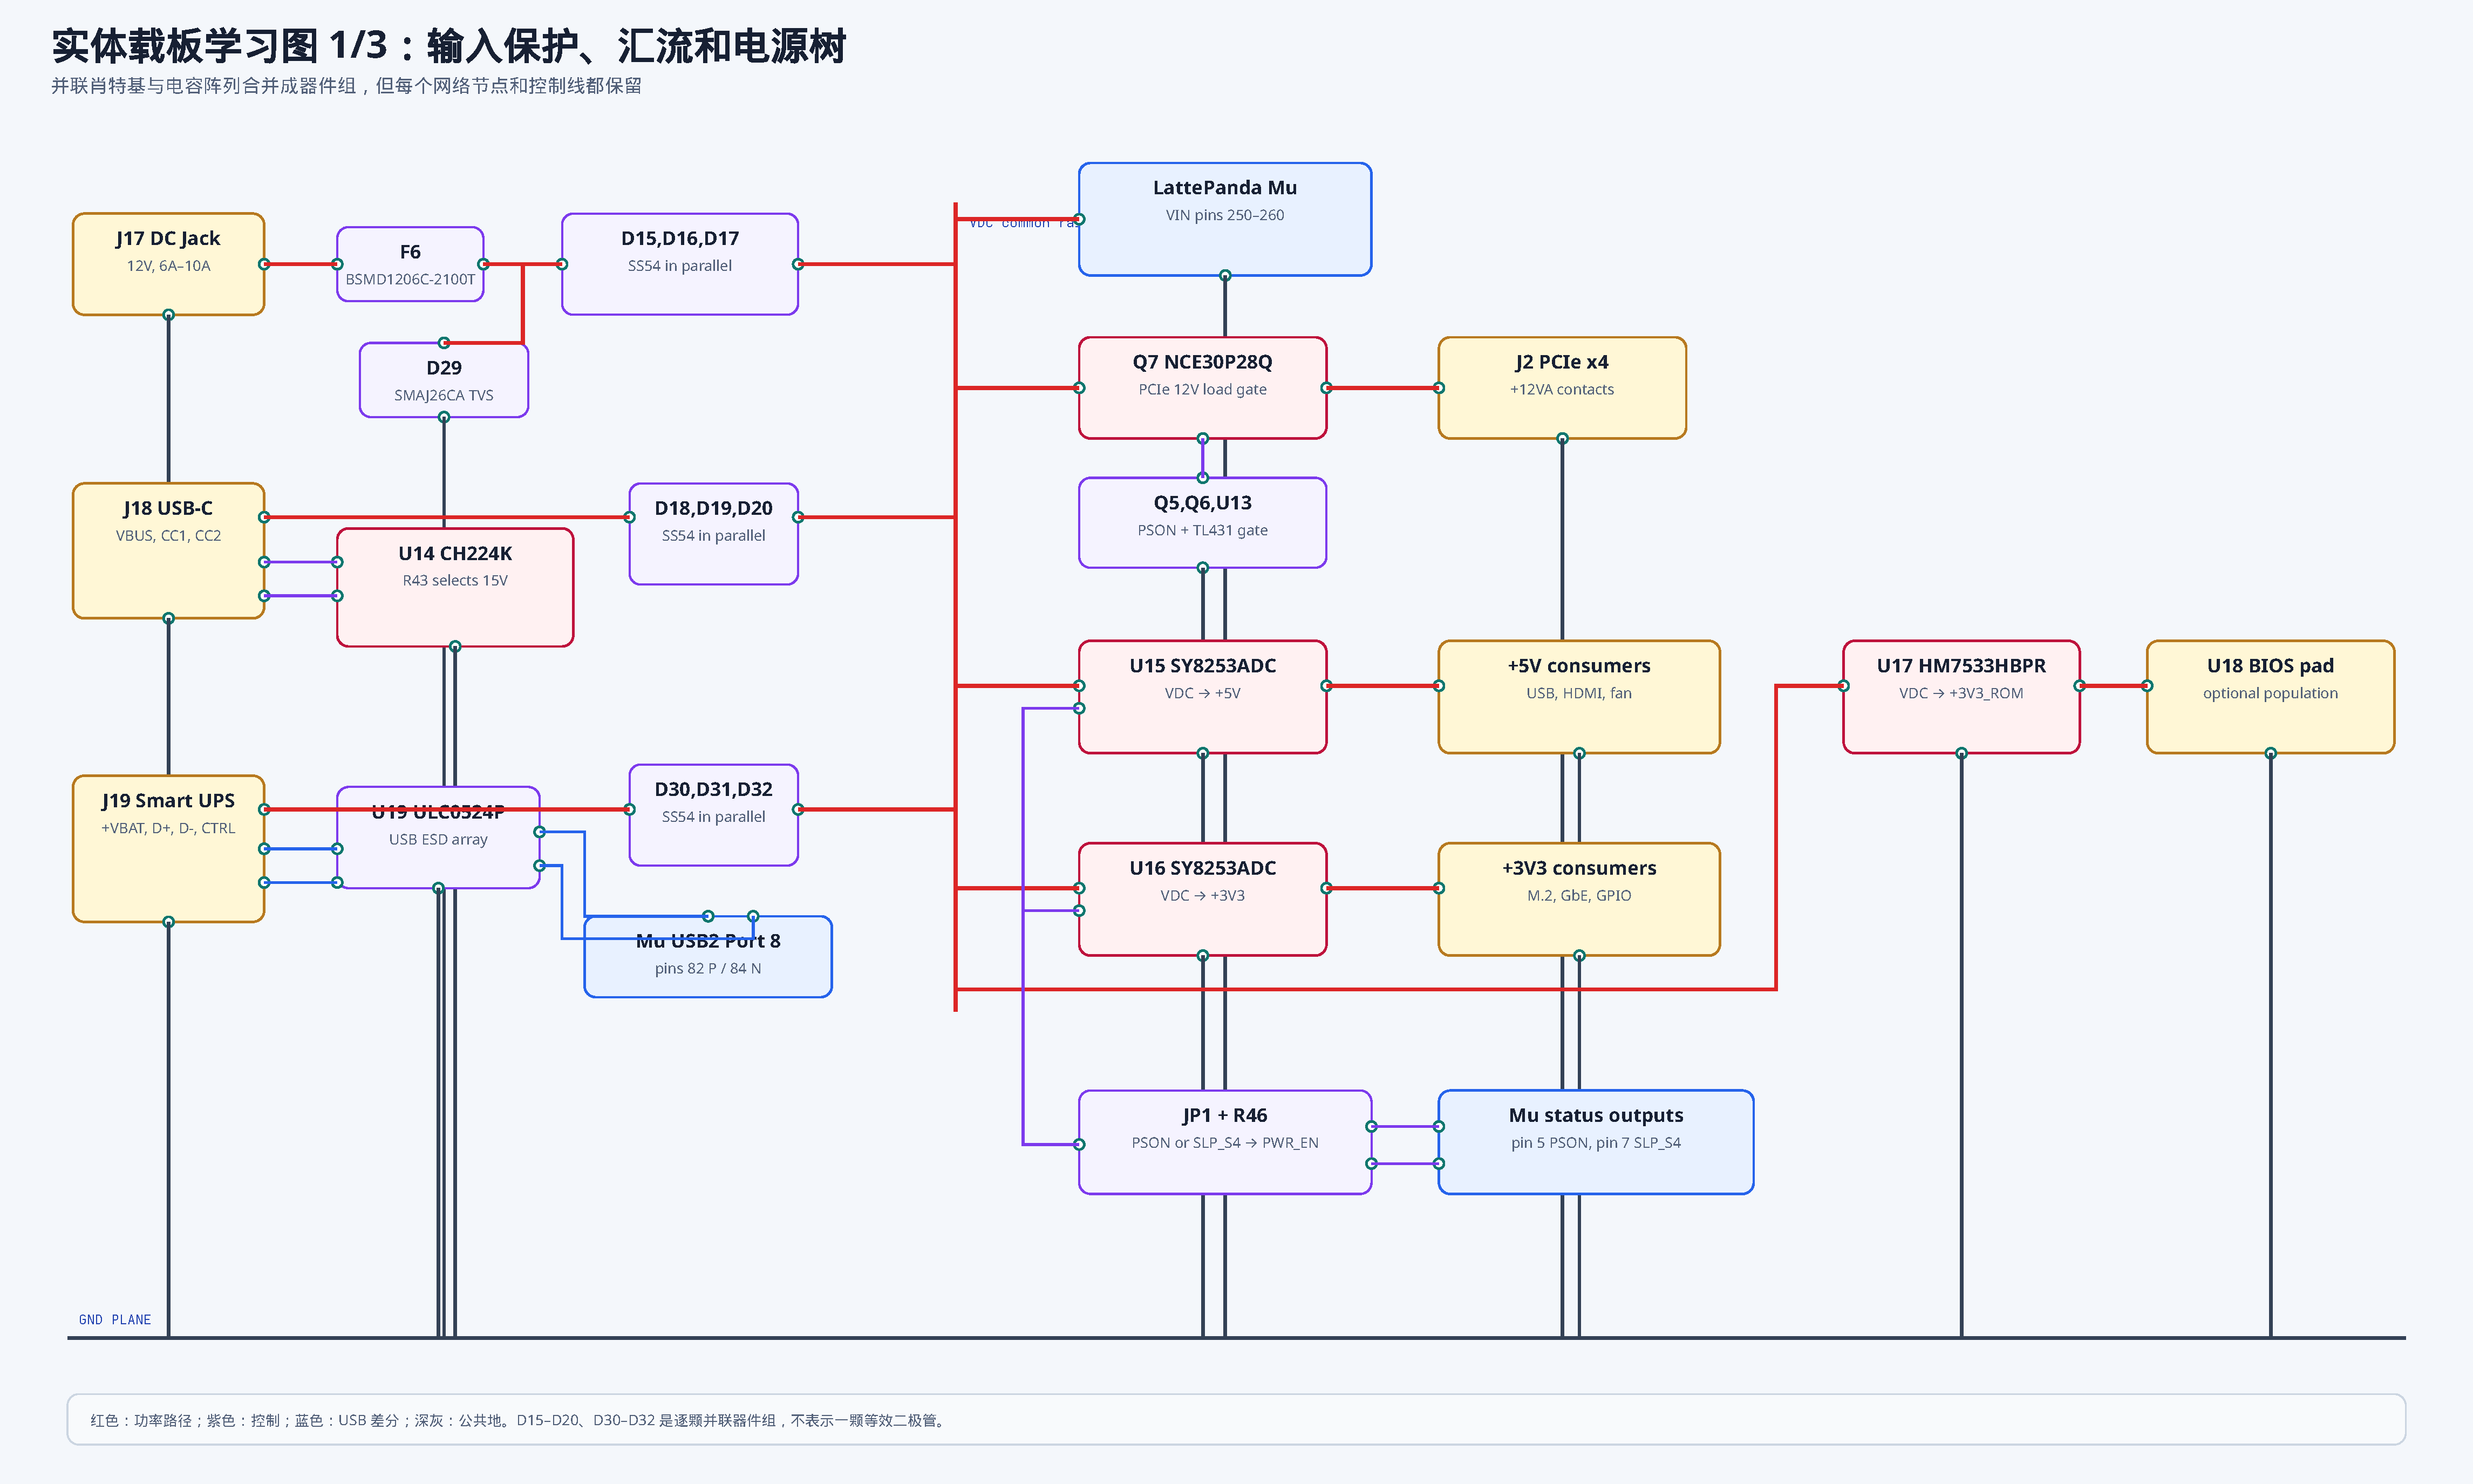
\includegraphics[width=\textwidth,height=0.82\textheight,keepaspectratio]
    {figures/physical_carrier/power_wiring.pdf}
  \caption{学习版电源全连线图：三路输入经保护和肖特基汇成 VDC，再进入模块、
  PCIe 12 V、5 V、3.3 V 和 ROM 3.3 V。}
  \label{fig:carrier-power-learning}
\end{figure}

\clearpage
\carrierschematicpage{9}{DFR1142 V2 原理图第 9 页：三路输入、降压、电源按键、
状态与 PCIe 12 V 的原始器件级电路。}{fig:carrier-power-original}

\topic{5.1 DC Jack：从 J17 到 VDC}
DC 圆孔插座 J17 的第 1 脚是正输入。正常电流路径为
\[
\mathrm{J17.1}
\rightarrow \mathrm{F6}
\rightarrow \code{DC\_FUSED}
\rightarrow \mathrm{D15\parallel D16\parallel D17}
\rightarrow \code{VDC}.
\]

F6 的型号是 \code{BSMD1206C-2100T}。它位于能量入口，在严重过流或短路
持续存在时限制能量，正常工作时应只有很小压降。保险丝不能代替正确
电源：输入过压未必产生足够电流使它及时动作。

D29 \code{SMAJ26CA} 从 \code{DC\_FUSED} 接到 GND，是
\term{TVS}{Transient Voltage Suppressor，瞬态电压抑制二极管}。正常电压
下它基本不参与；输入出现短时尖峰时，它快速导通，把电压钳位并将瞬态电流送回
地。TVS 必须靠近入口且回流低电感，否则尖峰在到达它之前已经作用于后级。

D15、D16、D17 是并联 SS54 肖特基二极管。\term{肖特基二极管}{正向压降较低、
开关较快的一类二极管}允许电流从 DC 输入流向 VDC，并阻止 VDC 反向灌回 DC
插座。三颗并联分担热量，但真实器件的正向压降有差异，电流不会理想地三等分；
PCB 铜形状应尽量对称，温升计算不能只把额定电流机械相加。

\topic{5.2 USB-C PD：协商电压不等于转换电压}
USB-C 插入时，电源适配器和受电设备先通过 CC1/CC2 判断方向、角色和可供能力。
U14 \code{CH224K} 根据 R43 配置向适配器请求 15 V。协商成功以后，J18 的
VBUS 才成为约 \code{+15V}，再经 D18、D19、D20 三颗 SS54 汇入 VDC：
\[
\mathrm{J18.CC1/CC2}
\rightarrow \mathrm{U14}
\Rightarrow \mathrm{VBUS}=15\mathrm{V}
\rightarrow \mathrm{D18\parallel D19\parallel D20}
\rightarrow \code{VDC}.
\]

\(\Rightarrow\) 表示 U14 用协议促成电源状态变化，不表示 CC 线上承载主功率。
CH224K 只负责协商，不执行降压；它请求支持的适配器直接提供 15 V。若适配器
不支持、CC 连接错误或配置不对，预期 VBUS 就不会出现。

\topic{5.3 Smart UPS：一只连接器同时承载四类职责}
J19 的 \code{+VBAT} pins 1/2 经 D30、D31、D32 汇入 VDC。它还带有：

\begin{itemize}[leftmargin=2em]
  \item USB D+/D-，经 U19 \code{ULC0524P} ESD 阵列接 Mu USB2 Port 8
        pins 82/84；
  \item \code{UPS\_STATE\_LP}，让模块读取 UPS 状态；
  \item \code{UPS\_SW\_LP}，让模块或按键控制 UPS；
  \item 多个地脚，提供功率和信号回流。
\end{itemize}

因此“UPS 接口”不是两根电池线。若只画电源而省略状态、控制、USB 和地，软件
将无法得到完整设备功能。

\topic{5.4 三路为什么能够汇合而不直接互灌}
每个输入都先经过朝向 VDC 的肖特基组，构成简单
\term{diode-OR}{用二极管让多个电源源端共同驱动一个负载端的汇流方式}。
某一路电压最高并足以正向偏置时，它向 VDC 供电；其余二极管因 VDC 较高而
反偏，减少输入之间的反灌。

这种方法简单，却不是无损“理想电源选择器”。二极管损耗近似
\[
P_{\mathrm{loss}}\approx I V_f,
\]
其中 \(V_f\) 是工作电流和温度下的正向压降。负载越大，发热越明显；并联不均
还会让某颗更热。设计验证必须检查最坏输入、电流、铜温升和器件温度。

\topic{5.5 VDC 的五条去路}\par
\begin{osgridlongtable}{L{0.18\linewidth}L{0.25\linewidth}L{0.24\linewidth}L{0.23\linewidth}}
分支 & 核心器件 & 输出/去向 & 为什么需要 \\ \hline
模块主输入 & 直接连接 & Mu pins 250--260 \code{VIN} & 模块接受 9--20 V，并联 11 个触点承载电流 \\ \hline
PCIe 12 V & Q7 \code{NCE30P28Q}、Q5/Q6/U13 & \code{+12VA} 到 J2 & 受控向扩展卡提供 12 V，而非把任意 VDC 直接送出 \\ \hline
5 V 降压 & U15 \code{SY8253ADC}、L1 & \code{+5V} & USB VBUS、HDMI 和风扇需要 5 V \\ \hline
3.3 V 降压 & U16 \code{SY8253ADC}、L2 & \code{+3V3} & M.2、RTL8111H 和低速接口需要 3.3 V \\ \hline
ROM 电源 & U17 \code{HM7533HBPR} & \code{+3V3\_ROM} & 为可选载板 SPI Flash 提供独立 3.3 V \\ \hline
\end{osgridlongtable}

“模块 VIN 允许 20 V”不能推出“PCIe 插槽可以接 20 V”。VIN 是模块输入规格；
PCIe 12 V 是另一个网络和协议要求。每个网络都要按自己的接收器额定值判断。

\topic{5.6 降压转换器为什么需要电感、电容和反馈}
\term{降压转换器}{buck converter}高速开关输入电压，通过电感和电容把脉冲
能量平均成较低直流输出。U15/U16 内部开关周期性连接输入，SW 节点驱动 L1/L2；
输出电容向负载提供瞬时电流并降低纹波；反馈电阻把输出的一小部分送回 FB，
控制器据此调整占空比。

电路形成两个同时重要的闭环：

\begin{enumerate}[leftmargin=2em]
  \item \textbf{能量回路}：输入电容、内部开关、SW、电感、输出电容、地返回；
  \item \textbf{控制回路}：输出电压、反馈分压、FB、控制器、开关占空比。
\end{enumerate}

PCB 上高 \(di/dt\) 输入热回路要尽量小，SW 铜皮要远离敏感反馈，FB 应从干净
输出点取样。原理图只声明连接关系，布局决定寄生电感、噪声和热是否可接受。

\topic{5.7 PWR\_EN 与“插电并不等于所有电源立即打开”}
JP1 在与 \code{PSON}、\code{SLP\_S4} 相关的状态之间提供配置，经 R46 形成
\code{PWR\_EN}，同时送到 U15/U16 的 EN。模块用电源状态信号表达 S0、睡眠
或关机阶段，载板据此放行或关闭外设电源。若软件请求关机却永远强制 EN 为高，
外设仍会耗电，状态机也会失去契约。

\begin{figure}[!htbp]
  \centering
  \begin{tikzpicture}[
      x=1cm,
      y=1cm,
      every node/.style={font=\footnotesize\sffamily},
      source/.style={
        draw=BookAmber,
        fill=BookAmber!18,
        rounded corners=1mm,
        minimum width=2.65cm,
        minimum height=0.8cm,
        align=center
      },
      stage/.style={
        draw=BookTeal,
        fill=BookTeal!10,
        rounded corners=1mm,
        minimum width=2.8cm,
        minimum height=0.8cm,
        align=center
      },
      module/.style={
        draw=BookBlue,
        fill=BookBlue!10,
        rounded corners=1mm,
        minimum width=3.1cm,
        minimum height=0.8cm,
        align=center
      },
      flow/.style={BookTeal,very thick,-{Latex[length=2mm]}},
      request/.style={BookBlue,thick,-{Latex[length=2mm]}},
      return/.style={BookRed,thick,-{Latex[length=2mm]}}
    ]
    \node[font=\bfseries\color{BookNavy}] at (6.6,5.55)
      {案例：功率进入模块以后，按键和状态线怎样决定外设电源};

    \node[source] (dc) at (1.4,4.5)
      {J17 DC\\F6、D15--D17};
    \node[source] (pd) at (1.4,3.3)
      {J18 USB-C PD\\U14、D18--D20};
    \node[source] (ups) at (1.4,2.1)
      {J19 UPS\\D30--D32};
    \node[stage] (vdc) at (4.6,3.3) {VDC 汇流点};
    \node[stage] (vin) at (7.8,3.3)
      {Mu VIN\\pins 250--260};
    \node[module] (pm) at (11.3,3.3)
      {模块内待机电源\\与平台状态机};

    \draw[flow] (dc.east) -| (vdc.west);
    \draw[flow] (pd.east) -- (vdc.west);
    \draw[flow] (ups.east) -| (vdc.west);
    \draw[flow] (vdc.east) -- (vin.west);
    \draw[flow,dashed] (vin.east) -- (pm.west);

    \node[source] (sw1) at (1.4,0.45)
      {SW1 瞬时拉低\\PWR\_SW\#};
    \node[stage] (pin1) at (4.6,0.45) {Mu pin 1};
    \draw[request] (sw1.east) -- (pin1.west);
    \draw[request,dashed] (pin1.east) -| (pm.south);

    \node[module] (state) at (11.3,1.45)
      {PSON pin 5\\SLP\_S4 pin 7};
    \node[stage] (enable) at (7.8,1.45)
      {JP1、R46\\形成 PWR\_EN};
    \node[source] (bucks) at (4.6,1.65)
      {U15/U16 使能\\建立 +5V、+3V3};
    \draw[return] (pm.south) -- (state.north);
    \draw[return] (state.west) -- (enable.east);
    \draw[return] (enable.west) -- (bucks.east);

    \node[font=\scriptsize\color{BookMuted},align=left,text width=12.3cm]
      at (6.6,-0.35) {
        实线是载板上的真实功率或控制网络；进入模块后的虚线表示公开资料只给出
        接口行为，没有给出模块内电源管理电路。按下 SW1 只是发出请求，
        U15/U16 是否开启取决于模块返回的状态线和 JP1 配置。
      };
  \end{tikzpicture}
  \caption{从三路输入到模块，再从模块状态返回载板稳压器的往返路径。它解释了
  为什么“VIN 已有电”和“USB、网卡等外设电源已经打开”是两个不同状态。}
  \label{fig:carrier-power-state-trace}
\end{figure}

\topic{5.8 USB 端口为什么各有自己的保险丝}
四个 USB VBUS 分别经 F2--F5 从 5 V 供电。F4/F5 为 6 V、2 A 类器件，
F2/F3 为 6 V、1 A 类器件。单端口短路时，独立保护可以限制故障向整个 5 V
轨扩散。数据线 ESD 保护和 VBUS 过流保护解决不同问题，不能互相替代。

\topic{六、260-pin 接口：载板与计算模块的总边界}\par
\carrierschematicpage{2}{DFR1142 V2 原理图第 2 页：260-pin Mu 模块连接器、
RTC、可选 SPI ROM 和全部跨页信号。}{fig:carrier-module-original}

图~\ref{fig:carrier-module-original} 看起来最密集，因为几乎所有功能都从这里
出发。不要按 1 到 260 死记；先按“电源和状态、HSIO、USB2、参考时钟、显示、
低速总线”分组。

\topic{6.1 最早期电源和控制脚}\par
\begin{osgridlongtable}{L{0.13\linewidth}L{0.21\linewidth}L{0.27\linewidth}L{0.29\linewidth}}
物理 pin & 信号 & 电气/方向 & 载板中的完整作用 \\ \hline
1 & \code{PWR\_SW\#} & 3.3 V 输入，内部约 10 k\(\Omega\) 上拉 & SW1 或外接按键拉低，请求模块改变电源状态 \\ \hline
3 & \code{RST\_SW\#} & 3.3 V 输入，内部约 10 k\(\Omega\) 上拉 & SW2 拉低，请求复位而非切断全部输入 \\ \hline
5 & \code{PSON} & 3.3 V 输出 & 表示活动电源状态，参与外设降压和状态灯控制 \\ \hline
7 & \code{SLP\_S4} & 3.3 V 输出 & 表示睡眠/软关机相关状态 \\ \hline
9 & \code{TSENSE} & 3.3 V 输入 & 可接 NTC 温度检测网络 \\ \hline
115 & \code{VBAT} & 约 3.0 V 后备电源 & CR1220 在主电源断开时维持 RTC/配置域 \\ \hline
131 & \code{SUSCLK} & 挂起时钟输出 & 向 M.2 等设备提供低功耗状态参考 \\ \hline
133 & \code{BIOS\_SEL} & 3.3 V 输入 & 选择模块集成固件或可选载板 SPI ROM 路径 \\ \hline
250--260 & \code{VIN} & 9--20 V 输入 & 11 个并联触点向模块传输主功率 \\ \hline
\end{osgridlongtable}

信号名后的 \code{\#} 表示低有效。例如内部上拉使 \code{PWR\_SW\#} 平时为高，
按键闭合后把它短时拉到 GND，模块检测到“有效”。按键不是直接承载 CPU 主电流，
它只向电源状态机发出请求。

\topic{6.2 为什么电源和地要占许多触点}
单个连接器触点有接触电阻和电流上限。多个 VIN 并联可降低等效阻抗和单点温升；
多个 GND 既承担功率返回，也穿插在高速对之间降低回流路径电感和串扰。删除
“重复地脚”会同时破坏供电和信号完整性。

\topic{6.3 HSIO 是可复用高速端口，不是固定接口名称}
\term{HSIO}{High-Speed I/O，高速输入输出}是模块发布的高速收发器资源。
同一组收发器能否配置成 PCIe、USB 或其他协议取决于 SoC 能力和 BIOS 配置。
PCB 铜线焊好后不会跟着固件改变去向，因此载板设计和 BIOS lane 配置必须锁定
为同一个系统方案。

\begin{osgridlongtable}{L{0.12\linewidth}L{0.32\linewidth}L{0.46\linewidth}}
HSIO & Mu 物理 pin & DFR1142 V2 实际用途 \\ \hline
0 & TX 13/15，RX 16/18 & USB 3.x 端口 1 的 SuperSpeed TX/RX \\ \hline
1 & TX 19/21，RX 22/24 & USB 3.x 端口 2 的 SuperSpeed TX/RX \\ \hline
2 & TX 25/27，RX 28/30 & M.2 M Key 的 PCIe x1 \\ \hline
3 & TX 31/33，RX 34/36 & M.2 E Key 的 PCIe x1 \\ \hline
6 & TX 61/63，RX 64/66 & RTL8111H 千兆网控制器的 PCIe x1 \\ \hline
8 & TX 37/39，RX 40/42 & PCIe x4 插槽 lane 0 \\ \hline
9 & TX 43/45，RX 46/48 & PCIe x4 插槽 lane 1 \\ \hline
10 & TX 49/51，RX 52/54 & PCIe x4 插槽 lane 2 \\ \hline
11 & TX 55/57，RX 58/60 & PCIe x4 插槽 lane 3 \\ \hline
\end{osgridlongtable}

\topic{七、高速线路为什么一定要画 P 和 N 两根}
\term{单端电压}以信号线相对参考地的电压解释状态；\term{差分电压}以 P、N
两线之差解释状态。若 P 比 N 高表示一种状态，N 比 P 高表示另一种状态。接收器
主要观察差值，因此两线共同受到的噪声有机会被抵消。

但差分对不是两根“随便保持差不多长”的普通线。发送器、走线和接收器组成传输线
系统，需要规定：

\begin{itemize}[leftmargin=2em]
  \item 单端和差分特性阻抗，以及允许误差；
  \item P/N 对内长度差和多 lane 之间的时延预算；
  \item 连续参考平面及换层时的回流过孔；
  \item 过孔、连接器、焊盘和 ESD 器件的寄生电容；
  \item 发送端 AC 耦合电容的位置和数值；
  \item 与开关电源、板边、平面开槽和其他高速线的间距。
\end{itemize}

\term{特性阻抗}{高速电磁波在传输线中看到的电压与电流关系}由线宽、线距、
铜厚、到参考平面的距离和介质常数共同决定，不等同于万用表测得的直流电阻。
信号边沿足够快时，即使板上只走几厘米，也必须按传输线而不是理想导线处理。

\term{AC 耦合电容}串在高速发送线上，阻断发送器和接收器之间的直流偏置，
让两端各自建立共模电压，而高速变化通过电容传递。它必须在协议规定的一侧，
不能看到“电容左右都通高速”就随意移动。DFR1142 中 PCIe 和 USB SuperSpeed
发送方向都明确放置耦合电容。

\begin{figure}[!htbp]
  \centering
  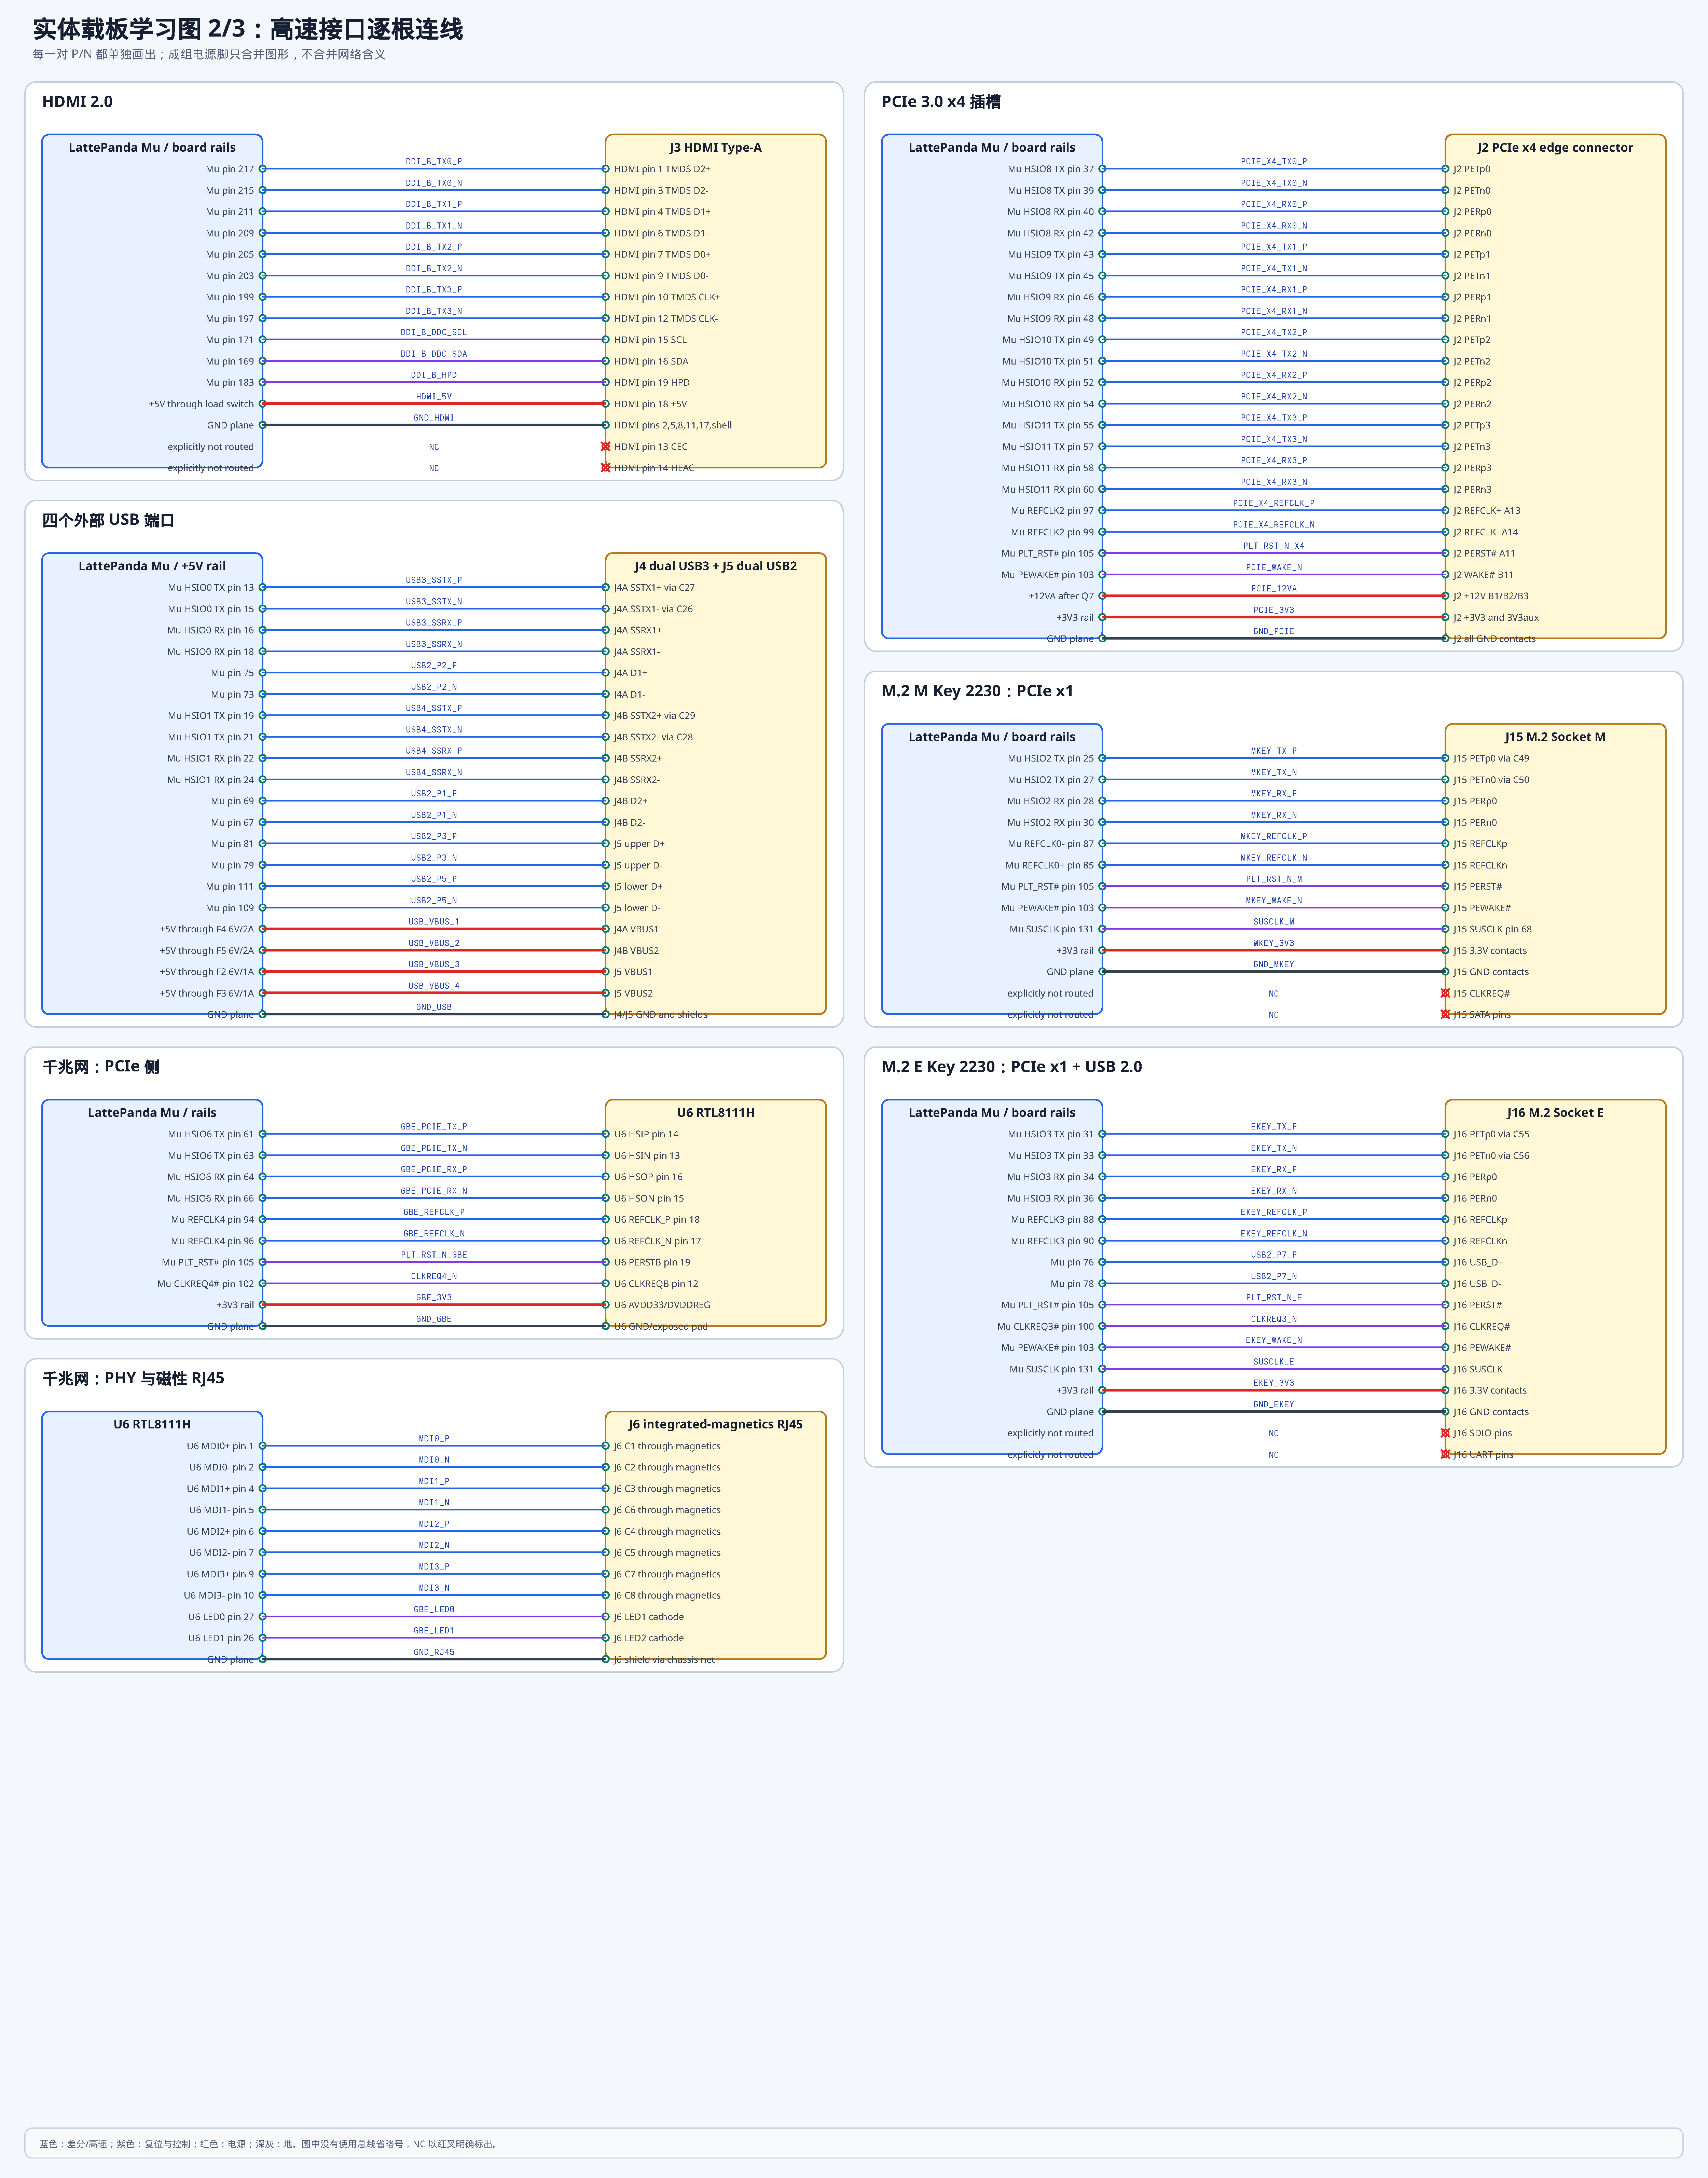
\includegraphics[width=\textwidth,height=0.88\textheight,keepaspectratio]
    {figures/physical_carrier/high_speed_wiring.pdf}
  \caption{学习版高速全连线图：每条 TX/RX P/N、参考时钟、复位、唤醒、电源与
  地均展开；粗略接口名没有替代实际铜线。}
  \label{fig:carrier-high-speed-learning}
\end{figure}

\topic{八、HDMI：显示数据之外还有发现与管理}\par
\carrierschematicpage{4}{DFR1142 V2 原理图第 4 页：HDMI TMDS、DDC、HPD、
5 V 与 ESD 保护。}{fig:carrier-hdmi-original}

HDMI Type-A 连接器 J3 看似“视频线”，启动时至少有三条不同性质的路径：

\begin{enumerate}[leftmargin=2em]
  \item 板端 5 V 和 HPD 让源端知道显示器是否连接；
  \item DDC 的 SCL/SDA 让源端用 I2C 类事务读取显示器 EDID 能力；
  \item 四对 TMDS 差分线传输像素数据与时钟。
\end{enumerate}

\begin{osgridlongtable}{L{0.24\linewidth}L{0.15\linewidth}L{0.23\linewidth}L{0.28\linewidth}}
Mu 信号 & pin & HDMI pin & 含义 \\ \hline
\code{DDI\_B\_TX0\_P/N} & 217/215 & 1/3 & TMDS Data2 P/N \\ \hline
\code{DDI\_B\_TX1\_P/N} & 211/209 & 4/6 & TMDS Data1 P/N \\ \hline
\code{DDI\_B\_TX2\_P/N} & 205/203 & 7/9 & TMDS Data0 P/N \\ \hline
\code{DDI\_B\_TX3\_P/N} & 199/197 & 10/12 & TMDS Clock P/N \\ \hline
\code{DDI\_B\_DDC\_SCL} & 171 & 15 & 读取 EDID 的时钟 \\ \hline
\code{DDI\_B\_DDC\_SDA} & 169 & 16 & 读取 EDID 的双向数据 \\ \hline
\code{DDI\_B\_HPD} & 183 & 19 & 显示器热插拔检测 \\ \hline
\code{HDMI\_5V} & 板上 5 V & 18 & HDMI 辅助 5 V \\ \hline
GND/Shield & 地网/机壳策略 & 2/5/8/11/17/外壳 & 差分回流、低速参考和屏蔽 \\ \hline
\end{osgridlongtable}

\begin{figure}[!htbp]
  \centering
  \begin{tikzpicture}[
      x=1cm,
      y=1cm,
      every node/.style={font=\footnotesize\sffamily},
      endpoint/.style={
        draw=BookBlue,
        fill=BookBlue!10,
        rounded corners=1mm,
        minimum width=2.7cm,
        minimum height=0.8cm,
        align=center
      },
      pins/.style={
        draw=BookTeal,
        fill=BookTeal!10,
        rounded corners=1mm,
        minimum width=4.1cm,
        minimum height=0.8cm,
        align=center
      },
      connector/.style={
        draw=BookAmber,
        fill=BookAmber!18,
        rounded corners=1mm,
        minimum width=3.2cm,
        minimum height=0.8cm,
        align=center
      },
      tx/.style={BookTeal,very thick,-{Latex[length=2mm]}},
      control/.style={
        BookBlue,
        thick,
        {Latex[length=2mm]}-{Latex[length=2mm]}
      },
      detect/.style={BookRed,thick}
    ]
    \node[font=\bfseries\color{BookNavy}] at (6.55,4.95)
      {案例：显示引擎不是只接四对 TMDS};
    \node[endpoint] (engine) at (1.45,3.75)
      {SoC 显示引擎\\DDI B};
    \node[pins] (tmds) at (6.55,3.75)
      {TX0/1/2/3 P/N\\Mu pins 197--217};
    \node[connector] (j3) at (11.65,3.75)
      {J3 HDMI\\pins 1--12};
    \draw[tx,dashed] (engine.east) -- (tmds.west);
    \draw[tx] (tmds.east) -- node[above]{四对 TMDS} (j3.west);

    \node[endpoint] (ddc-engine) at (1.45,2.45)
      {DDC 控制器\\读取 EDID};
    \node[pins] (ddc) at (6.55,2.45)
      {SCL pin 171\\SDA pin 169};
    \node[connector] (ddc-j3) at (11.65,2.45)
      {J3 pins 15/16\\显示器 DDC};
    \draw[control,dashed] (ddc-engine.east) -- (ddc.west);
    \draw[control] (ddc.east) -- (ddc-j3.west);

    \node[endpoint] (detect-engine) at (1.45,1.15)
      {热插拔检测\\与模式选择};
    \node[pins] (hpd) at (6.55,1.15)
      {HPD Mu pin 183\\HDMI\_5V 来自板上 +5V};
    \node[connector] (hpd-j3) at (11.65,1.15)
      {J3 pin 19 返回 HPD\\J3 pin 18 得到 5V};
    \draw[detect,dashed,<-] (detect-engine.east) -- (hpd.west);
    \draw[detect,<-] (hpd.east) -- (hpd-j3.west);

    \node[font=\scriptsize\color{BookMuted},align=center,text width=12.5cm]
      at (6.55,0.15) {
        插入显示器时先有 5 V、HPD 和 DDC 事务；固件或驱动读取 EDID 并选择模式后，
        显示引擎才在 TMDS 对上连续发送像素。三行是三种电气职责，不能合并成一根
        “HDMI 总线”。
      };
  \end{tikzpicture}
  \caption{从 SoC 显示功能到 Mu 引脚，再到 HDMI 连接器的三条并行路径。虚线
  只表示模块内功能归属，实线对应载板原理图第 4 页。}
  \label{fig:carrier-hdmi-trace}
\end{figure}

CEC pin 13 和 HEAC/reserved pin 14 明确 NC。它们出现在标准连接器上，不代表
本设计必须实现。学习图保留 NC 状态，是为了避免读者误以为“原图少画两根”。

\topic{软件怎样用到这些线}%
固件或图形驱动检测 HPD，经过 DDC 读取 EDID，选择显示模式，配置显示控制器，
最后才在 TMDS 对上传输图像。当前 STUOS 没有 DDI/HDMI 驱动；实体适配初期
更现实的方案是由 UEFI GOP 提供已初始化 framebuffer，再逐步开发原生驱动。

\topic{九、USB：一个 USB 3.x 插口其实同时有两套数据通道}\par
\carrierschematicpage{5}{DFR1142 V2 原理图第 5 页：两个 USB 3.x、两个
USB 2.0、独立 VBUS 保护和 ESD。}{fig:carrier-usb-original}

USB 3.x Type-A 插座既保留 USB 2.0 D+/D-，又增加一对 SuperSpeed TX 和
一对 SuperSpeed RX。兼容 USB 2.0 的设备只使用 D+/D-；SuperSpeed 设备还
使用额外四根高速单端铜线。高速失败而 D+/D- 正常时，设备可能降速但仍能工作，
这也是调试时必须分别检查两套通道的原因。

\begin{osgridlongtable}{L{0.13\linewidth}L{0.31\linewidth}L{0.27\linewidth}L{0.19\linewidth}}
端口 & SuperSpeed TX & SuperSpeed RX & USB 2.0 \\ \hline
J4A & HSIO0 pins 13/15，经 C27/C26 & HSIO0 pins 16/18 & Port 2 pins 75/73 \\ \hline
J4B & HSIO1 pins 19/21，经 C29/C28 & HSIO1 pins 22/24 & Port 1 pins 69/67 \\ \hline
J5 上层 & 无 & 无 & Port 3 D+ 81、D- 79 \\ \hline
J5 下层 & 无 & 无 & Port 5 D+ 111、D- 109 \\ \hline
\end{osgridlongtable}

C26--C29 均为 100 nF/16 V AC 耦合电容，位于模块的 SuperSpeed TX 方向。
RX 方向由对端发送器负责相应耦合，不能因为图形看起来对称便随意在每条线上重复
添加电容。

\begin{figure}[!htbp]
  \centering
  \begin{tikzpicture}[
      x=1cm,
      y=1cm,
      every node/.style={font=\footnotesize\sffamily},
      endpoint/.style={
        draw=BookBlue,
        fill=BookBlue!10,
        rounded corners=1mm,
        minimum width=2.8cm,
        minimum height=0.8cm,
        align=center
      },
      pins/.style={
        draw=BookTeal,
        fill=BookTeal!10,
        rounded corners=1mm,
        minimum width=3.5cm,
        minimum height=0.8cm,
        align=center
      },
      part/.style={
        draw=BookAmber,
        fill=BookAmber!18,
        rounded corners=1mm,
        minimum width=2.5cm,
        minimum height=0.8cm,
        align=center
      },
      bus/.style={BookTeal,very thick,-{Latex[length=2mm]}},
      duplex/.style={
        BookBlue,
        thick,
        {Latex[length=2mm]}-{Latex[length=2mm]}
      },
      supply/.style={BookRed,thick,-{Latex[length=2mm]}}
    ]
    \node[font=\bfseries\color{BookNavy}] at (6.6,5.5)
      {案例：J4A 同时连接 SuperSpeed、USB2 和端口电源};
    \node[endpoint] (xhci) at (1.4,4.2) {SoC xHCI\\与 USB PHY};
    \node[pins] (txpins) at (5.2,4.2)
      {HSIO0 TX\\pins 13/15};
    \node[part] (caps) at (8.5,4.2)
      {C27/C26\\100 nF};
    \node[part] (sstx) at (11.8,4.2)
      {J4A SSTX\\P/N};
    \draw[bus,dashed] (xhci.east) -- (txpins.west);
    \draw[bus] (txpins.east) -- (caps.west);
    \draw[bus] (caps.east) -- (sstx.west);

    \node[endpoint] (xhci-rx) at (1.4,2.95) {SoC SuperSpeed\\接收器};
    \node[pins] (rxpins) at (5.2,2.95)
      {HSIO0 RX\\pins 16/18};
    \node[part] (ssrx) at (11.8,2.95)
      {J4A SSRX\\P/N};
    \draw[bus,dashed,<-] (xhci-rx.east) -- (rxpins.west);
    \draw[bus,<-] (rxpins.east) -- (ssrx.west);
    \node[font=\scriptsize\color{BookMuted}] at (8.5,3.45)
      {接收方向不重复放 C26/C27};

    \node[endpoint] (usb2) at (1.4,1.7)
      {SoC USB2\\控制器/PHY};
    \node[pins] (usb2pins) at (5.2,1.7)
      {Port 2 D+/D-\\pins 75/73};
    \node[part] (esd) at (8.5,1.7)
      {低电容 ESD\\靠近插座};
    \node[part] (dpdm) at (11.8,1.7)
      {J4A D+/D-};
    \draw[duplex,dashed] (usb2.east) -- (usb2pins.west);
    \draw[duplex] (usb2pins.east) -- (esd.west);
    \draw[duplex] (esd.east) -- (dpdm.west);

    \node[endpoint] (five) at (1.4,0.45) {板上 +5V};
    \node[pins] (fuse) at (5.2,0.45)
      {该端口独立保险丝\\F2--F5 中的一路};
    \node[part] (vbus) at (11.8,0.45)
      {J4A VBUS\\与 GND 回流};
    \draw[supply] (five.east) -- (fuse.west);
    \draw[supply] (fuse.east) -- (vbus.west);
  \end{tikzpicture}
  \caption{一个 USB 3.x Type-A 插座的四条职责。高速发送、接收、USB2 和供电
  分别追线，便能区分“完全不枚举”“只能以 USB2 工作”和“端口没有 VBUS”。}
  \label{fig:carrier-usb-j4a-trace}
\end{figure}

每个插口的 VBUS 经独立保险丝从 5 V 获得，数据线靠近连接器经过低电容 ESD
器件。VBUS 提供设备电源；D+/D- 和 SuperSpeed 对传数据；GND 提供信号参考和
电流回流；金属外壳负责屏蔽与机械。这四类脚不能合并成一句“USB 接上模块”。

\topic{从插入键盘到内核收到按键}%
在实体机器上，USB 控制器首先检测连接和速度，分配地址，读取描述符，选择配置，
HID 驱动再周期读取或接收中断传输报告，最后把用法码转换为键盘事件。当前
STUOS 的键盘路径是 QEMU i8042/PS2 和 IRQ1，并没有 USB 主控制器枚举或 HID
栈，所以插到这块载板的 USB 键盘不会自动沿现有驱动工作。

\topic{十、PCIe x4：四条 lane、时钟、复位、唤醒和电源}\par
\carrierschematicpage{3}{DFR1142 V2 原理图第 3 页：PCIe 3.0 x4 插槽四条
lane、AC 耦合、参考时钟、控制与电源。}{fig:carrier-pcie-original}

\term{PCIe lane}{一条全双工 PCI Express 串行通道}包含一对发送 P/N 和一对
接收 P/N，即四根高速单端铜线。x4 插槽有四条 lane，因此仅数据部分就是
16 根高速铜线；此外还有差分参考时钟和若干低速控制。

\begin{osgridlongtable}{L{0.09\linewidth}L{0.29\linewidth}L{0.23\linewidth}L{0.29\linewidth}}
lane & Mu TX P/N 到插槽 & TX 耦合 & 插槽 TX 到 Mu RX P/N \\ \hline
0 & HSIO8 pins 37/39 到 \code{PETp0/PETn0} & C1/C2 & \code{PERp0/PERn0} 到 pins 40/42 \\ \hline
1 & HSIO9 pins 43/45 到 \code{PETp1/PETn1} & C3/C4 & \code{PERp1/PERn1} 到 pins 46/48 \\ \hline
2 & HSIO10 pins 49/51 到 \code{PETp2/PETn2} & C5/C6 & \code{PERp2/PERn2} 到 pins 52/54 \\ \hline
3 & HSIO11 pins 55/57 到 \code{PETp3/PETn3} & C7/C8 & \code{PERp3/PERn3} 到 pins 58/60 \\ \hline
\end{osgridlongtable}

名称 PET/PER 是从插槽/根端口视角定义的发送和接收。追线时永远先确定方向：
Mu 的 TX 必须到扩展设备的 RX，扩展设备 TX 必须回到 Mu RX。不能仅按两端都
有“TX”字样直接同名相接。

\begin{osgridlongtable}{L{0.24\linewidth}L{0.18\linewidth}L{0.48\linewidth}}
附加网络 & Mu pin/来源 & 完整作用 \\ \hline
\code{REFCLK2\_P/N} & 97/99 & 100 MHz 差分参考时钟，帮助链路两端建立共同频率基准 \\ \hline
\code{PLT\_RST\#} & 105 & 接插槽 \code{PERST\#}，平台未就绪时保持设备复位 \\ \hline
\code{PEWAKE\#} & 103 & 设备可请求从低功耗状态唤醒平台 \\ \hline
\code{+12VA} & Q7 受控输出 & 为需要 12 V 的扩展卡负载供电 \\ \hline
\code{+3V3} & U16 输出 & 提供 3.3 V 和辅助电源相关触点 \\ \hline
GND & 地平面 & 覆盖标准规定的所有返回触点和屏蔽参考 \\ \hline
\end{osgridlongtable}

\begin{figure}[!htbp]
  \centering
  \begin{tikzpicture}[
      x=1cm,
      y=1cm,
      every node/.style={font=\footnotesize\sffamily},
      endpoint/.style={
        draw=BookBlue,
        fill=BookBlue!10,
        rounded corners=1mm,
        minimum width=2.9cm,
        minimum height=0.82cm,
        align=center
      },
      group/.style={
        draw=BookTeal,
        fill=BookTeal!10,
        rounded corners=1mm,
        text width=4.25cm,
        minimum width=4.75cm,
        minimum height=0.82cm,
        align=center
      },
      slot/.style={
        draw=BookAmber,
        fill=BookAmber!18,
        rounded corners=1mm,
        minimum width=3.6cm,
        minimum height=0.82cm,
        align=center
      },
      forward/.style={BookTeal,very thick,-{Latex[length=2mm]}},
      backward/.style={BookBlue,very thick,{Latex[length=2mm]}-},
      control/.style={BookRed,thick,-{Latex[length=2mm]}}
    ]
    \node[font=\bfseries\color{BookNavy}] at (6.55,5.85)
      {案例：SoC 的四个 root-port lane 怎样落到 J2};
    \node[endpoint] (root) at (1.45,4.55)
      {SoC PCIe\\root complex};
    \node[group] (tx) at (6.35,4.55)
      {HSIO8--11 TX\\
       pins 37/39、43/45、49/51、55/57\\
       经 C1--C8 AC 耦合};
    \node[slot] (pet) at (11.65,4.55)
      {J2 PETp/n\\lane 0--3};
    \draw[forward,dashed] (root.east) -- (tx.west);
    \draw[forward] (tx.east) -- (pet.west);

    \node[endpoint] (root-rx) at (1.45,2.95)
      {SoC PCIe\\接收器};
    \node[group] (rx) at (6.35,2.95)
      {HSIO8--11 RX\\
       pins 40/42、46/48、52/54、58/60};
    \node[slot] (per) at (11.65,2.95)
      {J2 PERp/n\\lane 0--3};
    \draw[backward,dashed] (root-rx.east) -- (rx.west);
    \draw[backward] (rx.east) -- (per.west);

    \node[endpoint] (platform) at (1.45,1.35)
      {平台时钟、复位\\与电源管理};
    \node[group] (sideband) at (6.35,1.35)
      {REFCLK2 pins 97/99\\PLT\_RST\# 105，PEWAKE\# 103};
    \node[slot] (slot-sideband) at (11.65,1.35)
      {J2 REFCLK、PERST\#\\WAKE\#};
    \draw[control,dashed] (platform.east) -- (sideband.west);
    \draw[control] (sideband.east) -- (slot-sideband.west);

    \node[endpoint] (rails) at (1.45,0.1)
      {VDC/+3V3\\载板电源树};
    \node[group] (switch) at (6.35,0.1)
      {Q7 受控形成 +12VA\\U16 形成 +3V3};
    \node[slot] (slot-power) at (11.65,0.1)
      {J2 12V、3.3V\\与全部 GND};
    \draw[control] (rails.east) -- (switch.west);
    \draw[control] (switch.east) -- (slot-power.west);
  \end{tikzpicture}
  \caption{PCIe x4 不是一条粗线。四条发送 lane、四条接收 lane、参考时钟、
  复位、唤醒和电源分别到达 J2；其中只有发送方向的 C1--C8 位于本板。}
  \label{fig:carrier-pcie-x4-trace}
\end{figure}

\topic{复位释放后仍不能立刻把 PCIe 当内存用}%
根端口和设备先进行链路训练，协商速度和 lane 数。固件或内核随后枚举配置空间，
读取 vendor/device ID，分配 BAR 地址窗口，配置中断与总线主控，驱动才可使用
设备。铜线连通只是物理层前提，不等于操作系统已经拥有驱动。

\topic{十一、M.2 M Key 与 E Key 为什么不能只说“都是 M.2”}\par
\carrierschematicpage{8}{DFR1142 V2 原理图第 8 页：M.2 M Key 与 E Key 的
PCIe、USB、时钟、复位、唤醒和电源。}{fig:carrier-m2-original}

\term{M.2}同时规定机械尺寸、key 缺口位置、引脚和可选接口。Key 只限制可插
卡类型，不能单独保证主板真的接出了所有可能协议。本载板的 M Key 只接 PCIe
x1，不接 SATA；E Key 同时接 PCIe x1 和 USB 2.0，适合常见 Wi-Fi/蓝牙组合卡。

\topic{11.1 M Key：本设计是一条 PCIe x1}\par
\begin{osgridlongtable}{L{0.25\linewidth}L{0.35\linewidth}L{0.30\linewidth}}
功能 & Mu 来源 & J15 去向/状态 \\ \hline
PCIe TX P/N & HSIO2 pins 25/27，经 C49/C50 220 nF/16 V & \code{PETp0/PETn0} \\ \hline
PCIe RX P/N & HSIO2 pins 28/30 & \code{PERp0/PERn0} \\ \hline
参考时钟 & REFCLK0 pins 85/87，原图明确交换 P/N & \code{REFCLKp/n} \\ \hline
复位 & \code{PLT\_RST\#} pin 105 & \code{PERST\#} \\ \hline
唤醒 & \code{PEWAKE\#} pin 103 & \code{PEWAKE\#} \\ \hline
挂起时钟 & \code{SUSCLK} pin 131 & \code{SUSCLK} \\ \hline
供电 & \code{+3V3}/GND & 标准规定的全部供电与地触点 \\ \hline
未用 & 未从模块接出 & SATA 与 \code{CLKREQ\#} 明确 NC \\ \hline
\end{osgridlongtable}

\begin{figure}[!htbp]
  \centering
  \begin{tikzpicture}[
      x=1cm,
      y=1cm,
      every node/.style={font=\footnotesize\sffamily},
      module/.style={
        draw=BookBlue,
        fill=BookBlue!10,
        rounded corners=1mm,
        minimum width=3.15cm,
        minimum height=0.82cm,
        align=center
      },
      carrier/.style={
        draw=BookTeal,
        fill=BookTeal!10,
        rounded corners=1mm,
        minimum width=3.4cm,
        minimum height=0.82cm,
        align=center
      },
      device/.style={
        draw=BookAmber,
        fill=BookAmber!18,
        rounded corners=1mm,
        minimum width=3.1cm,
        minimum height=0.82cm,
        align=center
      },
      forward/.style={BookTeal,very thick,-{Latex[length=2mm]}},
      backward/.style={BookBlue,very thick,{Latex[length=2mm]}-},
      side/.style={BookRed,thick,-{Latex[length=2mm]}}
    ]
    \node[font=\bfseries\color{BookNavy}] at (6.55,5.55)
      {案例：M Key NVMe 卡的一次 PCIe 物理连接};
    \node[module] (root) at (1.55,4.25)
      {SoC PCIe root\\HSIO2 TX 25/27};
    \node[carrier] (caps) at (6.55,4.25)
      {C49/C50\\220 nF AC 耦合};
    \node[device] (nvme-rx) at (11.55,4.25)
      {J15 PETp0/n0\\NVMe 接收器};
    \draw[forward,dashed] (root.east) -- (caps.west);
    \draw[forward] (caps.east) -- (nvme-rx.west);

    \node[module] (root-rx) at (1.55,2.95)
      {SoC PCIe RX\\HSIO2 pins 28/30};
    \node[carrier] (direct-rx) at (6.55,2.95)
      {载板直接布线\\本方向无 C49/C50};
    \node[device] (nvme-tx) at (11.55,2.95)
      {J15 PERp0/n0\\NVMe 发送器};
    \draw[backward,dashed] (root-rx.east) -- (direct-rx.west);
    \draw[backward] (direct-rx.east) -- (nvme-tx.west);

    \node[module] (platform) at (1.55,1.35)
      {REFCLK0 85/87\\原图交换 P/N\\PLT\_RST\# 105};
    \node[carrier] (j15-side) at (6.55,1.35)
      {J15 REFCLKp/n\\PERST\#、PEWAKE\#};
    \node[device] (nvme-side) at (11.55,1.35)
      {NVMe 时钟、复位\\与唤醒逻辑};
    \draw[side] (platform.east) -- (j15-side.west);
    \draw[side] (j15-side.east) -- (nvme-side.west);

    \node[module] (software) at (1.55,-0.05)
      {CPU 写 NVMe doorbell\\并读取完成队列};
    \node[carrier] (bar) at (6.55,-0.05)
      {PCIe 配置空间、BAR\\与 DMA 地址};
    \node[device] (controller) at (11.55,-0.05)
      {NVMe 控制器\\提交/完成队列};
    \draw[BookMuted,thick,dashed,-{Latex[length=2mm]}]
      (software.east) -- (bar.west);
    \draw[BookMuted,thick,dashed,-{Latex[length=2mm]}]
      (bar.east) -- (controller.west);
  \end{tikzpicture}
  \caption{M.2 M Key 上的 NVMe 案例。上三行是载板接线，最后一行是链路训练和
  枚举以后才成立的软件事务；机械插入本身不会自动产生 BAR 和队列。}
  \label{fig:carrier-mkey-nvme-trace}
\end{figure}

参考时钟 P/N 交换是原设计明确记录的选择，不能推广为所有差分对可任意交换。
某些接收器或协议允许极性反转并在训练中恢复，另一些不允许；每条网络必须查询
对应规范和器件能力。

\topic{11.2 E Key：PCIe 常给 Wi-Fi，USB 常给蓝牙}\par
\begin{osgridlongtable}{L{0.25\linewidth}L{0.35\linewidth}L{0.30\linewidth}}
功能 & Mu 来源 & J16 去向/状态 \\ \hline
PCIe TX P/N & HSIO3 pins 31/33，经 C55/C56 220 nF/16 V & \code{PETp0/PETn0} \\ \hline
PCIe RX P/N & HSIO3 pins 34/36 & \code{PERp0/PERn0} \\ \hline
参考时钟 & REFCLK3 pins 88/90 & \code{REFCLKp/n} \\ \hline
USB 2.0 & Port 7 pins 76/78 & \code{USB\_D+/USB\_D-} \\ \hline
时钟请求 & \code{CLKREQ3\#} pin 100 & \code{CLKREQ\#} \\ \hline
复位/唤醒 & pins 105/103 & \code{PERST\#}/\code{PEWAKE\#} \\ \hline
挂起时钟 & \code{SUSCLK} pin 131 & \code{SUSCLK} \\ \hline
供电 & \code{+3V3}/GND & 标准规定的全部供电与地触点 \\ \hline
未用 & 未从模块接出 & SDIO、UART 明确 NC \\ \hline
\end{osgridlongtable}

若组合卡的 Wi-Fi 枚举而蓝牙不出现，应检查 USB2 路径；若蓝牙出现而 Wi-Fi
不出现，应检查 PCIe lane、参考时钟、复位和固件枚举。把两项都归为“无线坏了”
会丢失最重要的分层证据。

\section{网络、低速总线与板级辅助电路}

\carrierschematicpage{6}{DFR1142 V2 原理图第 6 页：RTL8111H 的 PCIe 端、
四对 MDI、磁性 RJ45、时钟、供电和 LED。}{fig:carrier-ethernet-original}

U6 \code{RTL8111H} 一侧是主机 PCIe 接口，另一侧集成以太网 MAC/PHY 功能并
输出四对 MDI。它把两套完全不同的电气和协议域连接起来。

\begin{osgridlongtable}{L{0.28\linewidth}L{0.15\linewidth}L{0.47\linewidth}}
Mu 网络 & pin & RTL8111H 端及职责 \\ \hline
HSIO6 TX P/N & 61/63 & \code{HSIP/HSIN}，主机向网卡的 PCIe 高速数据 \\ \hline
HSIO6 RX P/N & 64/66 & \code{HSOP/HSON}，网卡向主机的 PCIe 高速数据 \\ \hline
\code{REFCLK4\_P/N} & 94/96 & PCIe 参考时钟 \\ \hline
\code{PLT\_RST\#} & 105 & \code{PERSTB}，保持网卡复位直到平台放行 \\ \hline
\code{CLKREQ4\#} & 102 & \code{CLKREQB}，电源管理时请求参考时钟 \\ \hline
\end{osgridlongtable}

网线侧有 MDI0--MDI3 共四对双绞线，先进入 J6 内置隔离磁性器件，再到 RJ45
触点。磁性器件提供交流耦合、共模抑制和电气隔离，不能为了“少几个器件”把 PHY
直接接到长网线。J6 的 LED0/LED1 显示 link/activity；金属外壳与数字 GND、
机壳地之间的处理还影响 ESD 与 EMC。

\begin{figure}[!htbp]
  \centering
  \begin{tikzpicture}[
      x=1cm,
      y=1cm,
      every node/.style={font=\footnotesize\sffamily},
      block/.style={
        draw=BookBlue,
        fill=BookBlue!10,
        rounded corners=1mm,
        minimum width=2.45cm,
        minimum height=0.9cm,
        align=center
      },
      boundary/.style={
        draw=BookTeal,
        fill=BookTeal!10,
        rounded corners=1mm,
        minimum width=2.55cm,
        minimum height=0.9cm,
        align=center
      },
      hardware/.style={
        draw=BookAmber,
        fill=BookAmber!18,
        rounded corners=1mm,
        minimum width=2.55cm,
        minimum height=0.9cm,
        align=center
      },
      data/.style={
        BookTeal,
        very thick,
        {Latex[length=2mm]}-{Latex[length=2mm]}
      },
      side/.style={BookRed,thick,-{Latex[length=2mm]}}
    ]
    \node[font=\bfseries\color{BookNavy}] at (6.55,4.9)
      {案例：一帧数据跨过 PCIe 域和以太网线缆域};
    \node[block] (root) at (1.25,3.55)
      {SoC PCIe root\\与 DMA/APIC};
    \node[boundary] (hsio6) at (4.7,3.55)
      {HSIO6 TX 61/63\\RX 64/66};
    \node[hardware] (rtl) at (8.15,3.55)
      {U6 RTL8111H\\PCIe + MAC/PHY};
    \node[hardware] (mag) at (11.6,3.55)
      {J6 内置磁性\\四对 MDI};
    \draw[data,dashed] (root.east) -- (hsio6.west);
    \draw[data] (hsio6.east) -- (rtl.west);
    \draw[data] (rtl.east) -- (mag.west);

    \node[block] (clock) at (1.25,1.95)
      {平台时钟\\与复位控制};
    \node[boundary] (pins) at (4.7,1.95)
      {REFCLK4 94/96\\PLT\_RST\# 105};
    \node[hardware] (rtl-side) at (8.15,1.95)
      {U6 REFCLK\\PERSTB/CLKREQB};
    \node[hardware] (cable) at (11.6,1.95)
      {RJ45 触点\\双绞网线};
    \draw[side,dashed] (clock.east) -- (pins.west);
    \draw[side] (pins.east) -- (rtl-side.west);
    \draw[data] (mag.south) |- (cable.north);

    \node[
      draw=BookMuted,
      fill=white,
      rounded corners=1mm,
      align=left,
      text width=11.9cm
    ] at (6.55,0.45) {
      左半段传输 PCIe 事务，右半段传输以太网物理符号。RTL8111H 在中间完成
      协议和电气域转换。收包时 U6 通过 DMA 写 RAM，再由中断通知 CPU；
      发包时 CPU/驱动准备描述符，U6 读取内存并从四对 MDI 发出。
    };
  \end{tikzpicture}
  \caption{CPU 到真实网口的接线链。PCIe lane 只到 RTL8111H，网线并不直接
  连到 CPU；磁性器件也不是可省略的“普通连接器内部导线”。}
  \label{fig:carrier-ethernet-trace}
\end{figure}

\topic{从一包网络数据到用户程序的完整链}%
网线电压波形经磁性器件进入 PHY，PHY 恢复符号和帧，RTL8111H 经 DMA 把数据
写入 RAM 并触发中断，驱动回收描述符，网络栈解析以太网/IP/传输层，最后把
字节交给进程。当前 STUOS 没有 PCIe 枚举、RTL8111H 驱动、DMA 或网络栈，
所以真实网口焊接完整不等于当前内核已经能联网。

\topic{十三、I2C、UART、SPI 和控制线从零解释}\par
\begin{figure}[!htbp]
  \centering
  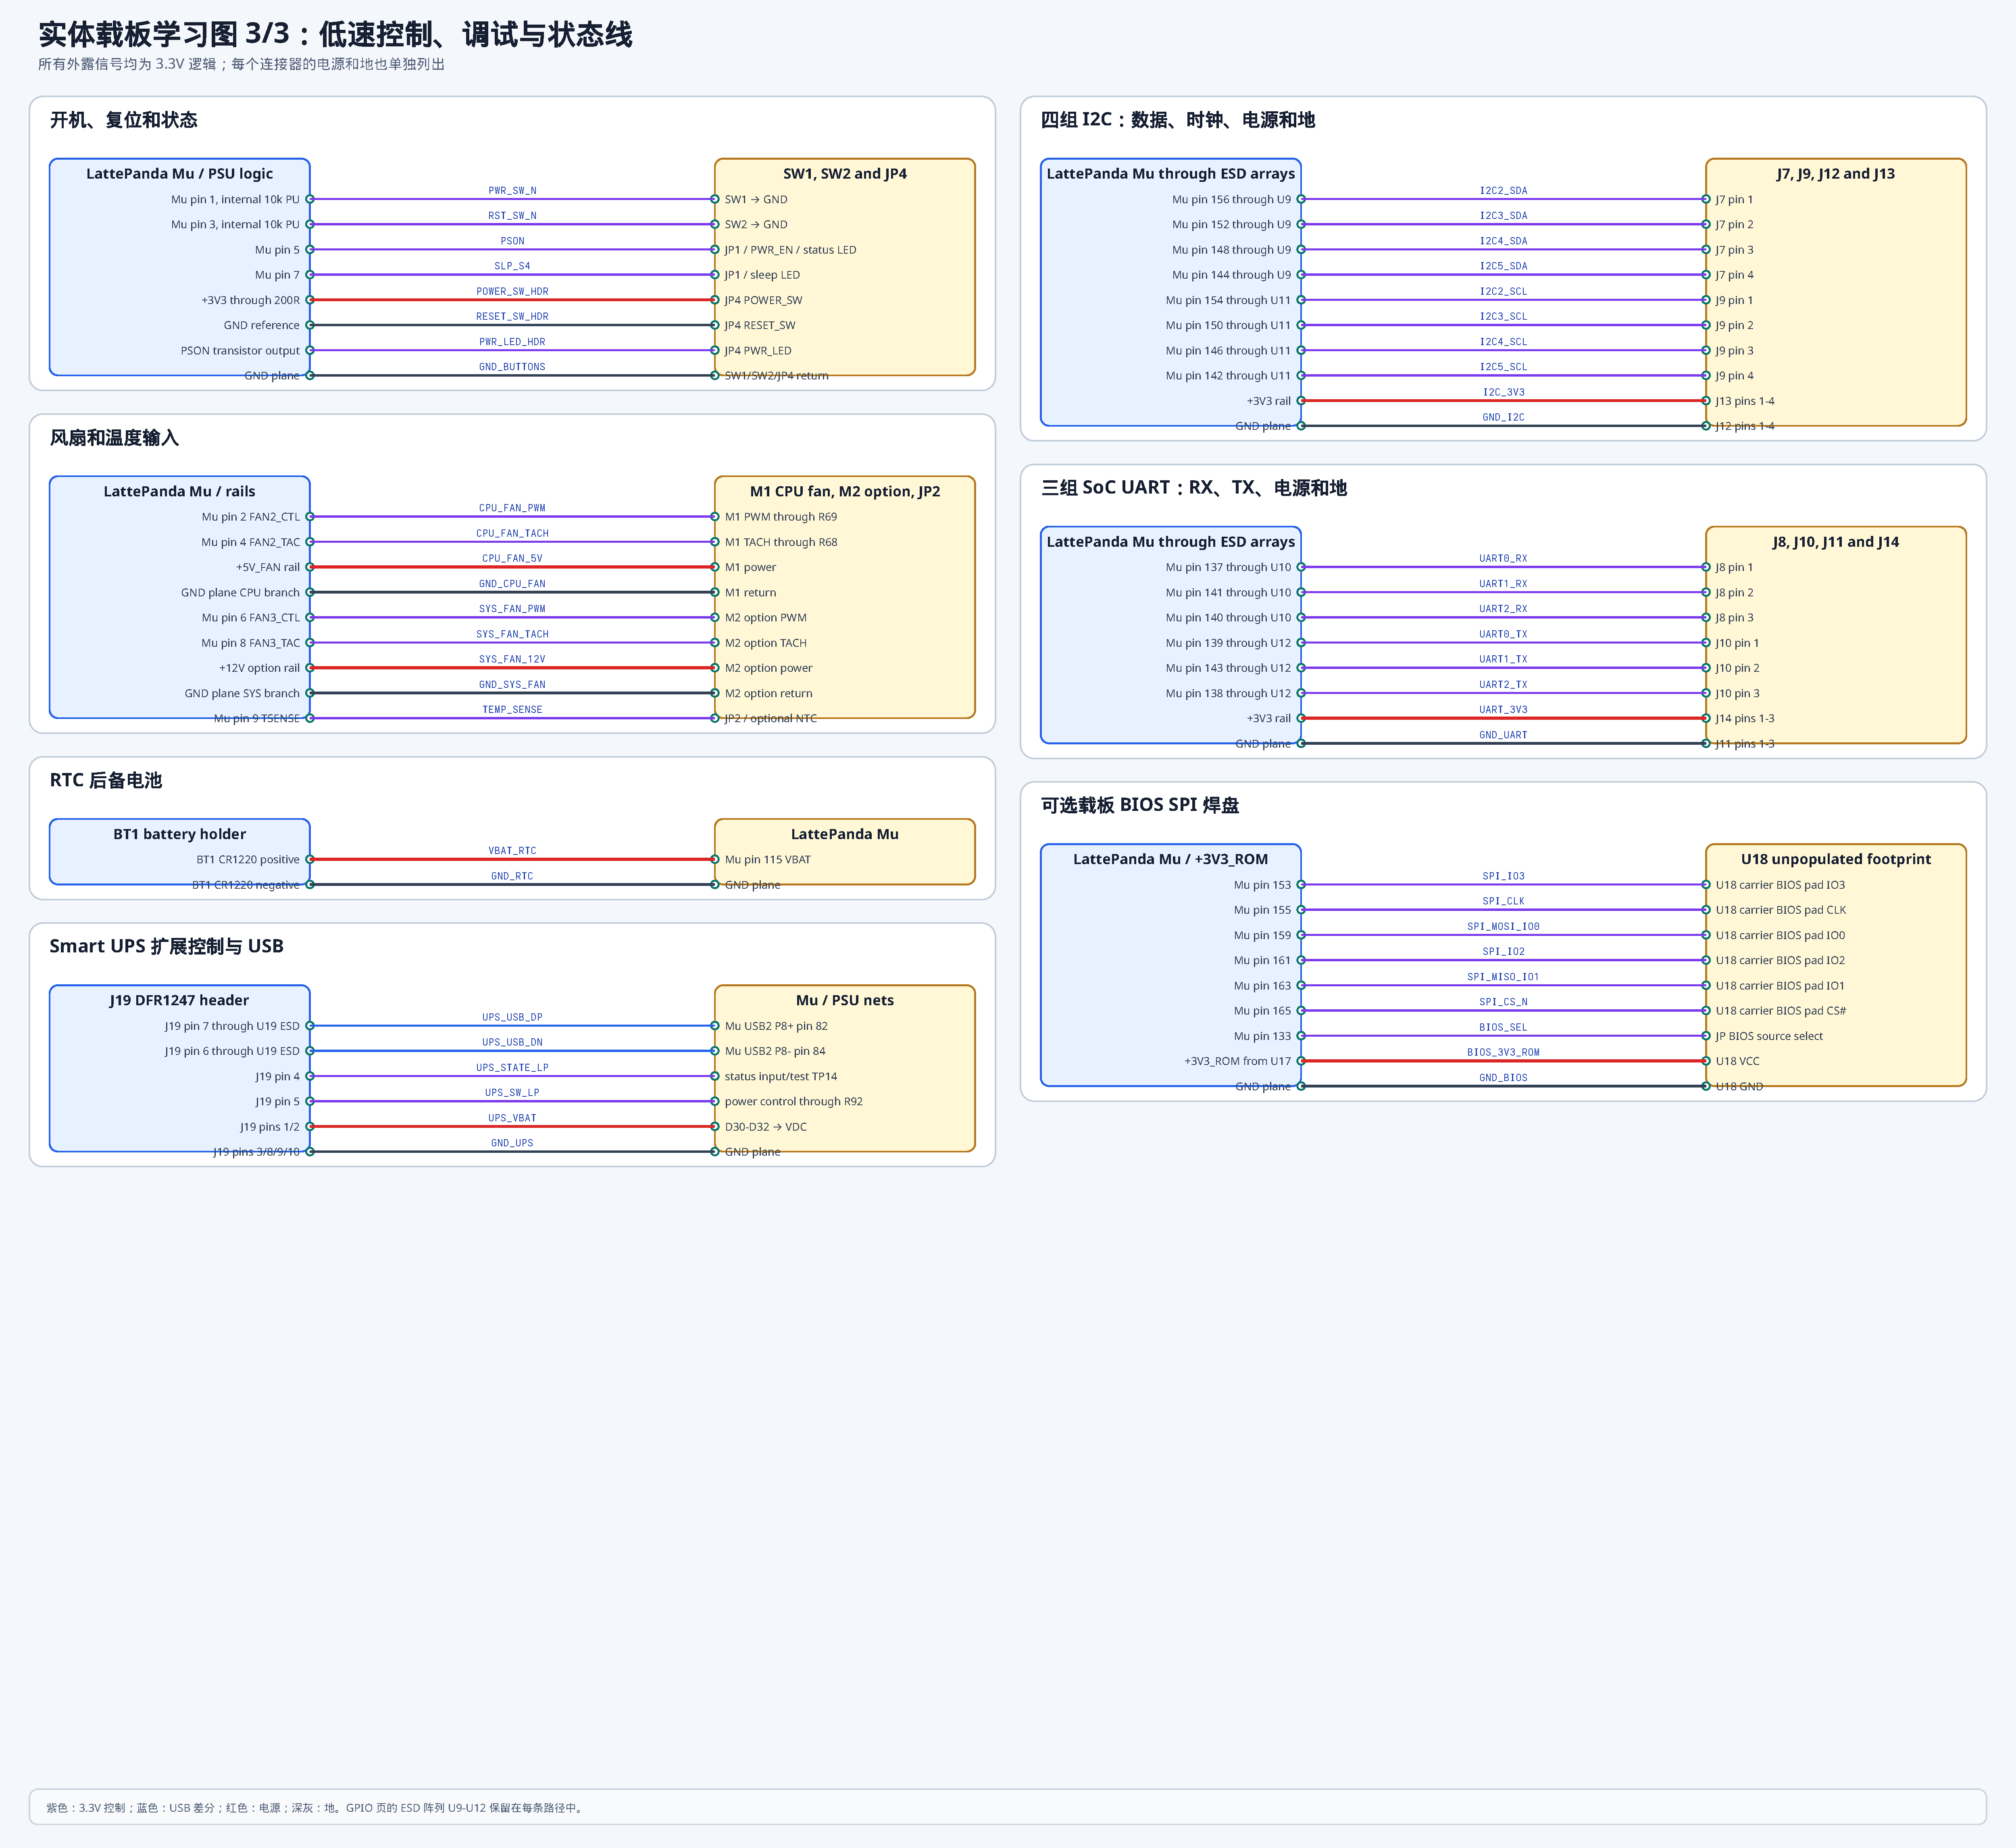
\includegraphics[width=\textwidth,height=0.86\textheight,keepaspectratio]
    {figures/physical_carrier/control_wiring.pdf}
  \caption{学习版低速全连线图：按键、状态、风扇、RTC、UPS、四组 I2C、三组
  UART 与可选 SPI ROM 的每根信号、电源和地。}
  \label{fig:carrier-control-learning}
\end{figure}

\carrierschematicpage{7}{DFR1142 V2 原理图第 7 页：GPIO、四组 I2C、三组
UART、电源/地排针和 ESD。}{fig:carrier-low-speed-original}

\topic{13.1 I2C：两根共享线为什么需要上拉}
\term{I2C}{Inter-Integrated Circuit}通常用 SCL 时钟和 SDA 数据两根信号线
连接一个控制器与多个有地址的设备。许多 I2C 输出采用
\term{开漏}{器件只能主动拉低，释放时不主动拉高}结构。总线靠上拉电阻回到
高电平，因此多个器件可以共享线路而不让一个强推高、另一个强拉低。

一次典型事务包含起始条件、地址与读写位、接收方应答、若干数据字节和停止条件。
“地址”在这里是总线设备编号，不是 CPU 物理地址。上拉阻值与总线电容决定
上升时间；并联太多外设上拉会让等效阻值过低，拉低电流增大。Mu 内部已有约
2.2 k\(\Omega\) 上拉，不能不计算就反复添加。

\begin{osgridlongtable}{L{0.15\linewidth}L{0.32\linewidth}L{0.33\linewidth}}
总线 & SCL 来源/排针 & SDA 来源/排针 \\ \hline
I2C2 & Mu pin 154 到相应 J9 pin 1 & Mu pin 156 到相应 J7 pin 1 \\ \hline
I2C3 & Mu pin 150 到相应 J9 pin 2 & Mu pin 152 到相应 J7 pin 2 \\ \hline
I2C4 & Mu pin 146 到相应 J9 pin 3 & Mu pin 148 到相应 J7 pin 3 \\ \hline
I2C5 & Mu pin 142 到相应 J9 pin 4 & Mu pin 144 到相应 J7 pin 4 \\ \hline
\end{osgridlongtable}

SCL/SDA 经 U9/U11 ESD 阵列，J13 提供四个 +3V3，J12 提供四个 GND。一个外设
至少要有电源、地、SCL 和 SDA；只接两根“数据线”没有完整参考和供电。

\topic{13.2 UART：异步串行不等于 RS-232 电平}
\term{UART}{Universal Asynchronous Receiver/Transmitter}把并行字节变成
按时间发送的串行位。常见帧包含起始位、若干数据位、可选校验位和停止位。
双方没有共享时钟线，所以必须预先约定波特率和帧格式。

本载板 UART 是 3.3 V CMOS/TTL 类逻辑。传统 RS-232 使用正负高电压且逻辑
极性定义也不同，必须通过电平转换器；把 DB9 RS-232 直接接到 Mu 引脚可能
损坏输入。

\begin{osgridlongtable}{L{0.15\linewidth}L{0.31\linewidth}L{0.31\linewidth}}
UART & RX 到 J8 & TX 到 J10 \\ \hline
UART0 & Mu pin 137 到 pin 1 & Mu pin 139 到 pin 1 \\ \hline
UART1 & Mu pin 141 到 pin 2 & Mu pin 143 到 pin 2 \\ \hline
UART2 & Mu pin 140 到 pin 3 & Mu pin 138 到 pin 3 \\ \hline
\end{osgridlongtable}

J14 提供 +3V3，J11 提供 GND，U10/U12 提供 ESD 保护。调试线连接时要交叉
方向：板的 TX 接 USB-UART 适配器 RX，板的 RX 接适配器 TX，两边 GND 相连，
并确认都是 3.3 V 逻辑。

\begin{figure}[!htbp]
  \centering
  \begin{tikzpicture}[
      x=1cm,
      y=1cm,
      every node/.style={font=\footnotesize\sffamily},
      module/.style={
        draw=BookBlue,
        fill=BookBlue!10,
        rounded corners=1mm,
        minimum width=2.55cm,
        minimum height=0.78cm,
        align=center
      },
      protection/.style={
        draw=BookTeal,
        fill=BookTeal!10,
        rounded corners=1mm,
        minimum width=2.35cm,
        minimum height=0.78cm,
        align=center
      },
      external/.style={
        draw=BookAmber,
        fill=BookAmber!18,
        rounded corners=1mm,
        minimum width=2.7cm,
        minimum height=0.78cm,
        align=center
      },
      tx/.style={BookTeal,very thick,-{Latex[length=2mm]}},
      rx/.style={BookBlue,very thick,{Latex[length=2mm]}-},
      ground/.style={BookMuted,thick}
    ]
    \node[font=\bfseries\color{BookNavy}] at (6.55,4.65)
      {案例：UART0 调试线为什么必须交叉 TX/RX};
    \node[module] (soc-tx) at (1.35,3.45)
      {SoC UART0 TX\\Mu pin 139};
    \node[protection] (tx-esd) at (4.55,3.45)
      {U10/U12\\ESD 路径};
    \node[protection] (j10) at (7.75,3.45)
      {J10 pin 1\\板端 TX};
    \node[external] (adapter-rx) at (11.45,3.45)
      {USB-UART\\适配器 RX};
    \draw[tx,dashed] (soc-tx.east) -- (tx-esd.west);
    \draw[tx] (tx-esd.east) -- (j10.west);
    \draw[tx] (j10.east) -- (adapter-rx.west);

    \node[module] (soc-rx) at (1.35,2.15)
      {SoC UART0 RX\\Mu pin 137};
    \node[protection] (rx-esd) at (4.55,2.15)
      {U10/U12\\ESD 路径};
    \node[protection] (j8) at (7.75,2.15)
      {J8 pin 1\\板端 RX};
    \node[external] (adapter-tx) at (11.45,2.15)
      {USB-UART\\适配器 TX};
    \draw[rx,dashed] (soc-rx.east) -- (rx-esd.west);
    \draw[rx] (rx-esd.east) -- (j8.west);
    \draw[rx] (j8.east) -- (adapter-tx.west);

    \node[module] (module-ground) at (1.35,0.85)
      {Mu/载板 GND};
    \node[protection] (j11) at (7.75,0.85)
      {J11 GND};
    \node[external] (adapter-ground) at (11.45,0.85)
      {适配器 GND};
    \draw[ground] (module-ground.east) -- (j11.west);
    \draw[ground] (j11.east) -- (adapter-ground.west);

    \node[font=\scriptsize\color{BookRed},align=left,text width=11.7cm]
      at (6.55,-0.15) {
        J14 的 +3V3 用于给外接低功耗逻辑提供参考或受控电源，不表示可以把
        适配器的 5 V TX 接到 Mu。连接前先确认适配器 I/O 是 3.3 V，
        再连接 TX、RX 和共同地。
      };
  \end{tikzpicture}
  \caption{UART0 的实际调试接线。箭头沿发送方向画出，因此上行从 Mu 到适配器，
  下行从适配器回到 Mu；同名 TX 对 TX 的接法会让两端都在发送、无人接收。}
  \label{fig:carrier-uart0-debug-trace}
\end{figure}

\topic{13.3 SPI 与可选载板固件 Flash}
\term{SPI}{Serial Peripheral Interface}常用时钟、片选和双向数据线进行同步
串行传输。经典命名有 SCLK、CS、MOSI、MISO；SPI NOR Flash 还可把数据脚扩展
为 IO0--IO3，实现双线或四线传输。

载板为可选外部 ROM 预留以下接口：

\begin{osgridlongtable}{L{0.16\linewidth}L{0.30\linewidth}L{0.44\linewidth}}
Mu pin & 信号 & 作用 \\ \hline
153 & \code{SPI\_IO3} & 四线模式数据位 3 \\ \hline
155 & \code{SPI\_CLK} & 串行时钟 \\ \hline
159 & \code{SPI\_MOSI/IO0} & 主机输出/数据位 0 \\ \hline
161 & \code{SPI\_IO2} & 四线模式数据位 2 \\ \hline
163 & \code{SPI\_MISO/IO1} & 主机输入/数据位 1 \\ \hline
165 & \code{SPI\_CS\#} & 低有效片选 \\ \hline
133 & \code{BIOS\_SEL} & 选择集成或载板 ROM 路径 \\ \hline
电源 & \code{+3V3\_ROM}/GND & U17 提供的专用供电和返回 \\ \hline
\end{osgridlongtable}

该 footprint 默认 DNP。即使焊上兼容 Flash，也不能把当前 STUOS 的 128 KiB
QEMU ROM 原样写入后期待启动，因为实体模块固件还承担硅初始化、DRAM 训练、
HSIO 配置和 UEFI 服务；现有教学 ROM没有这些平台代码和签名/布局契约。

\topic{十四、RTC、按键、状态和风扇不是边角功能}\par
\carrierschematicpage{10}{DFR1142 V2 原理图第 10 页：CPU/SYS 风扇的 5 V、
PWM、TACH、可选温度输入及保护。}{fig:carrier-fan-original}

\term{RTC}{Real-Time Clock，实时时钟}在主电源断开时仍需保留时间和少量平台
状态。CR1220 的正极通过 \code{VBAT} 接 Mu pin 115，负极接 GND。电池不是
给整机继续运行，只给极低功耗后备域供电；极性接反、短路或使用错误电池都有
安全风险。

SW1 把 \code{PWR\_SW\#} 拉低，SW2 把 \code{RST\_SW\#} 拉低。前者向电源管理
状态机请求开关机，后者请求复位。长按电源键、操作系统软关机和瞬时复位可能
触发不同路径，不能只写成“都是重启”。

\term{PWM}{Pulse-Width Modulation，脉宽调制}用固定频率下高电平所占比例
表达控制量，模块用它调节风扇目标转速。\term{TACH}{tachometer，转速反馈}
由风扇输出脉冲，模块根据单位时间内脉冲数判断实际转速。PWM 是模块到风扇，
TACH 是风扇到模块，方向相反。

\begin{osgridlongtable}{L{0.24\linewidth}L{0.15\linewidth}L{0.51\linewidth}}
功能 & Mu pin & 外部连接与意义 \\ \hline
CPU 风扇 PWM & 2 & 到 M1 控制输入，只允许匹配的 3.3 V 逻辑 \\ \hline
CPU 风扇 TACH & 4 & M1 转速反馈到模块输入 \\ \hline
SYS 风扇 PWM & 6 & 到可选 M2 控制输入 \\ \hline
SYS 风扇 TACH & 8 & 可选 M2 转速反馈 \\ \hline
温度输入 & 9 & JP2/可选 NTC，用阻值随温度变化形成模拟测量 \\ \hline
风扇电源 & \code{+5V}/GND & 提供电机能量与返回，不能从 PWM 信号脚取电 \\ \hline
\end{osgridlongtable}

\section{PCB、软硬件边界与分阶段 bring-up}

原理图回答“应该相连什么”，PCB 回答“铜实际怎样连接”。本工程有 305 个
footprint、407 个网络、3961 段走线和 1307 个过孔，板框
\(146\ \mathrm{mm}\times102\ \mathrm{mm}\)。约 \(1.6062\ \mathrm{mm}\)
叠层为：

\begin{center}
\begin{osgridtabular}{lll}
从顶到底 & 铜/介质 & 主要学习职责 \\ \hline
F.Cu & \(35\ \mu\mathrm{m}\) 铜 & 顶层器件和短连接 \\ \hline
Prepreg & \(0.2104\ \mathrm{mm}\) & 决定顶层到参考平面的几何关系 \\ \hline
In1.Cu & \(15.2\ \mu\mathrm{m}\) 铜 & 主要连续 GND 参考与回流 \\ \hline
Core & \(1.065\ \mathrm{mm}\) & 主介质厚度 \\ \hline
In2.Cu & \(15.2\ \mu\mathrm{m}\) 铜 & 电源分配和辅助参考 \\ \hline
Prepreg & \(0.2104\ \mathrm{mm}\) & 决定底层到内层的几何关系 \\ \hline
B.Cu & \(35\ \mu\mathrm{m}\) 铜 & 底层器件、走线和铜皮 \\ \hline
\end{osgridtabular}
\end{center}

\topic{四层并不自动等于高速合格}%
差分阻抗需要板厂实际介质常数、压合厚度、铜厚、线宽和线距计算。高速线换层时，
信号电流通过过孔换层，回流也要有邻近地过孔完成参考转换。若线跨过地平面开槽，
回流被迫绕路，环路面积、辐射和串扰都会增加。

\topic{去耦电容为什么必须靠近电源脚}%
负载在极短时间内改变电流时，远处稳压器和长铜线的电感来不及供能。靠近 IC
电源脚的小电容提供局部瞬时电流，再由较大电容和稳压器在较慢时间尺度补回。
原理图上把电容接在同一 3.3 V 网络只说明直流逻辑连通，PCB 距离和回路面积
决定高频是否有效。

\topic{ESD 器件为什么靠连接器而不是靠模块}%
\term{ESD}{Electrostatic Discharge，静电放电}脉冲从外部连接器进入。保护
器件越靠近入口，脉冲越早被引到参考路径；若先让它沿长线穿过整板再钳位，
沿途器件和铜线已经承受高压。ESD 选型还要考虑高速结电容，保护更强但电容太大
也可能损坏信号眼图。

\topic{原理图、PCB 和成品分别能看见什么}%
\begin{osgridlongtable}{L{0.17\linewidth}L{0.32\linewidth}L{0.41\linewidth}}
观察位置 & 能看见什么 & 还需要检查什么 \\ \hline
原理图 & 网络意图、器件值、方向和接口 & footprint 映射、实际阻抗、机械干涉 \\ \hline
PCB 文件 & 焊盘、铜线、叠层、布局与设计规则 & 制造厂是否按数据生产、装配是否正确 \\ \hline
成品测量 & 电压、波形、温升、枚举和真实行为 & 未测工况的长期可靠性与全部规范裕量 \\ \hline
\end{osgridlongtable}

本书使用的构建环境没有 \code{kicad-cli}，因此这里不把 ERC/DRC 标为已通过。
上游参考工程也没有提供可直接采购的完整 BOM、CPL 与 Gerber。正式投板前仍要
重新检查库、物料、封装、阻抗、ERC/DRC、机械、热和法规要求。

\topic{十六、十页图的阅读路线与故障问题}\par
\begin{osgridlongtable}{L{0.08\linewidth}L{0.23\linewidth}L{0.31\linewidth}L{0.28\linewidth}}
页 & 先追哪条链 & 正常条件 & 失败时先问 \\ \hline
1 & 模块到每个功能页 & 所有跨页标签有唯一去向 & 网络名是否拼写一致、方向是否清楚 \\ \hline
2 & VIN/控制/HSIO 分组 & 模块 pin 与引脚表一致 & BIOS 复用是否与铜线方案一致 \\ \hline
3 & PCIe lane 0 再复制到 1--3 & TX/RX、时钟、复位、电源齐全 & 哪一 lane 未训练，PERST 是否释放 \\ \hline
4 & HPD、DDC、TMDS & 先发现显示器再传像素 & 5 V、HPD、EDID 还是高速数据失败 \\ \hline
5 & 单个 USB 3.x 端口两套通道 & VBUS、D+/D-、TX/RX 都存在 & 完全不枚举还是只降到 USB2 \\ \hline
6 & PCIe 到 RTL8111H 再到 RJ45 & 主机侧与网线侧分别成立 & PCIe 不枚举、PHY 无 link 或软件无驱动 \\ \hline
7 & 一组 I2C/UART 连电源地 & 电平、方向、上拉和 ESD 正确 & 是否误接 RS-232、是否缺共同地 \\ \hline
8 & M Key 和 E Key 分开追 & 实际接出协议匹配所插卡 & 卡要求 SATA/USB 而载板没有接出吗 \\ \hline
9 & 输入到 VDC 再到各电源轨 & 保护、汇流、使能、反馈依次成立 & 故障停在入口、EN、稳压还是负载短路 \\ \hline
10 & 5 V/PWM/TACH 三类线 & 能量、控制、反馈方向各自正确 & 风扇不转还是转速反馈不读 \\ \hline
\end{osgridlongtable}

\topic{十七、当前 STUOS 与实体载板的共同点和断层}
两台机器都执行 x86-64，都有物理地址、分页、异常、中断和设备，也都必须在
内核之前建立固件环境。两者使用不同的平台契约和设备集合，虚拟机同样需要
明确的硬件知识。

\begin{osgridlongtable}{L{0.25\linewidth}L{0.31\linewidth}L{0.34\linewidth}}
层次 & 当前 STUOS/QEMU & Mu N100/N305 实体平台 \\ \hline
机器定义 & \code{pc,accel=tcg} & SoC、模块固件、ACPI 和真实载板拓扑 \\ \hline
复位固件 & 自研 128 KiB ROM 映射到 4 GiB 顶端 & 模块厂商 UEFI/BIOS 完成硅与 DRAM 初始化 \\ \hline
主存说明 & QEMU 建立 RAM，项目另取 \code{fw\_cfg} E820 & UEFI Memory Map 与固件/ACPI 表 \\ \hline
磁盘 & legacy IDE/ATA PIO，端口 \code{0x1F0} & 主要可能是 NVMe、eMMC 或 USB \\ \hline
早期控制台 & 16550A COM1，端口 \code{0x3F8} & 需确认 UART 路径或使用 UEFI GOP framebuffer \\ \hline
定时与中断 & 8259A、PIT、i8042，加本地 APIC 路径 & APIC、ACPI、HPET/SoC 定时器和 USB HID 等 \\ \hline
设备发现 & 固定教学地址和少量约定 & PCI/PCIe 枚举、ACPI 命名设备和固件资源 \\ \hline
输入 & QEMU 注入 PS/2，经 i8042 IRQ1 & 实际常用 USB 键盘，需要 xHCI 与 HID 栈 \\ \hline
启动装入 & Stage 1 自行 ATA 读取容器/ELF & 初期更适合 UEFI 文件/块协议装入 PE/COFF 入口 \\ \hline
\end{osgridlongtable}

\topic{为什么不能把 128 KiB ROM 直接烧进 U18}%
QEMU 在创建机器时已经替我们建立了可用 RAM、指定设备模型和高端 ROM 映射。
Mu 模块上电则需要平台固件执行受厂商约束的电源、微码、DRAM、HSIO 和安全
初始化。U18 只是可选 SPI 固件路径的一部分，不会把缺失的 N100 平台初始化
自动补齐。错误固件还可能让模块不再启动。

\topic{接到真实主板前还要补哪些信号与限制}%
\begin{enumerate}[leftmargin=2em]
  \item 增加 UEFI PE/COFF 入口或一个边界明确的 UEFI 引导层；
  \item 读取 UEFI Memory Map，退出 Boot Services 前固定内存所有权；
  \item 解析 ACPI RSDP、MADT、MCFG 以及所选定时器相关表；
  \item 枚举 PCI/PCIe 配置空间并分配/接受固件分配的 BAR；
  \item 选择可验证的早期控制台：UEFI GOP 或确实接出且配置正确的 UART；
  \item 支持 NVMe、eMMC 或 USB 中至少一种实体启动存储路径；
  \item 为 USB 键盘增加 xHCI 和 HID，或先提供另一种输入路径；
  \item 保留现有 QEMU 自研 ROM 路线为独立教学平台，不用 UEFI 偷换其复位实验。
\end{enumerate}

\topic{18.1 从按下电源键到内核入口}\par
\begin{enumerate}[leftmargin=2em]
  \item DC、USB-PD 或 UPS 经过保护和二极管组建立 VDC。
  \item VDC 经 11 个 VIN 触点进入模块，模块内部待机电源与管理状态机运行。
  \item SW1 把 Mu pin 1 \code{PWR\_SW\#} 拉低，发出开机请求。
  \item 模块依照电源时序建立 SoC/DRAM 电源和时钟，保持并最终释放复位。
  \item 平台固件从模块固件存储取指，完成硅初始化、DRAM 训练和 HSIO 配置。
  \item UEFI 枚举 PCIe、USB、显示和启动介质，形成内存图与 ACPI 表。
  \item STUOS 的 UEFI 适配入口被装入 RAM，取得固件提供的图形/文件/块服务。
  \item 引导层取得最终 Memory Map，退出 Boot Services，把资源所有权交给内核。
  \item 内核建立自己的 GDT、IDT、页表、中断控制与驱动，随后启动用户程序。
\end{enumerate}

这条链明确区分了“板上有电”“CPU 已解除复位”“固件正在运行”“RAM 可用”
“设备已枚举”和“内核已接管”。看到风扇转只证明某些电源和控制已经活动，不能
证明内核入口已经执行。

\topic{18.2 从 USB 键盘到 Shell 字符}\par
\[
\begin{aligned}
&\text{按键机械动作}
\rightarrow \text{键盘微控制器生成 HID 报告}\\
&\rightarrow \text{USB D+/D- 或 SuperSpeed 物理传输}
\rightarrow \text{xHCI 控制器写 RAM 队列}\\
&\rightarrow \text{APIC 中断}
\rightarrow \text{xHCI 驱动回收传输描述符}
\rightarrow \text{HID 驱动解析用法码}\\
&\rightarrow \text{内核输入 FIFO 唤醒等待线程}
\rightarrow \text{fd 0 读取}
\rightarrow \text{Ring 3 Shell}.
\end{aligned}
\]

现有 QEMU 路径把中间部分替换为 PS/2、i8042 和 IRQ1。因此用户态 Shell 和
文件描述符抽象可以复用，硬件入口驱动不能原样复用。操作系统分层的价值就在于
把“字符事件”以上的语义与具体 USB/PS2 线路分开。

\topic{18.3 从 NVMe 文件到可运行进程}\par
\[
\begin{aligned}
\text{M.2 PCIe 物理链路}
&\rightarrow \text{PCIe 枚举与 BAR}
\rightarrow \text{NVMe 管理/IO 队列}
\rightarrow \text{DMA 到 RAM}\\
&\rightarrow \text{块缓存与文件系统}
\rightarrow \text{ELF 装载}
\rightarrow \text{页表与用户上下文}.
\end{aligned}
\]

每个箭头都有所有权和失败语义：BAR 必须不冲突，DMA 缓冲区必须在设备可访问
范围且生命周期未结束，完成队列必须与提交队列匹配，文件数据要通过格式与校验，
ELF 段权限要进入页表。不能把“NVMe SSD 插在 M.2 上”直接跳写成“内核能运行
程序”。

\topic{十九、从不上电到分阶段 bring-up}
\term{bring-up}{把新硬件从未验证状态逐级带到可工作的工程过程}必须限制每次
新增的不确定量。以下顺序用于理解，不替代具体板卡安全规范。

\begin{enumerate}[leftmargin=2em]
  \item \textbf{目检与文档核对}：确认板版本、极性、器件方向、焊桥、连接器和
        模块机械方向；对照 BOM/原理图而不是凭丝印猜。
  \item \textbf{断电阻值}：不装模块时测 VDC、5 V、3.3 V 对地阻值，排查近似
        短路；注意电容充电会让读数变化。
  \item \textbf{限流输入}：使用受控限流电源，只验证输入保护和待机路径，观察
        异常电流、发热和气味。
  \item \textbf{PD 协商}：若走 USB-C，确认 U14 实际请求并得到 15 V，不凭
        连接器外形推断。
  \item \textbf{电源树}：测 VDC、PWR\_EN、5 V、3.3 V、+3V3\_ROM 的静态值、
        启动顺序和纹波。
  \item \textbf{装模块开机}：继续限流与温度观察，检查 PWR\_SW、PSON、SLP\_S4
        和复位状态。
  \item \textbf{最小输出}：先取得固件 UART 或 HDMI/GOP 证据，再增加存储和
        扩展卡。
  \item \textbf{逐接口枚举}：每次只增加一个 USB、M.2 或 PCIe 设备，保存
        vendor/device ID、链路速度、错误计数和日志。
  \item \textbf{负载与热}：在功能成立以后再测试持续功率、纹波、链路误码、
        风扇控制和环境温度裕量。
\end{enumerate}

\begin{failurebox}
示波器探头地夹通常与保护地相连。若把它夹到并非安全地参考的节点，可能短路
电源或形成地环路。测量前必须知道仪器、电脑 USB、电源负极和被测板之间的接地
关系；不确定时由有经验人员复核。
\end{failurebox}

\topic{二十、读完后手算一次整条启动路径}
合上前面的图，尝试只用纸笔回答下面问题：

\begin{enumerate}[leftmargin=2em]
  \item RAM 为什么需要供电和初始化，ROM/Flash 为什么能解决第一条指令来源？
  \item 为什么 260-pin SODIMM 外形不能推出它是 DDR4 内存条接口？
  \item DC、USB-PD、UPS 怎样进入 VDC，又怎样避免直接互相反灌？
  \item CH224K 完成的是协议协商还是降压？U15/U16 又完成什么？
  \item 为什么模块 VIN 可到 20 V，不表示 PCIe 插槽可接受 20 V？
  \item 一条 PCIe lane 有几根高速铜线，x4 的数据线总数为何是 16？
  \item 为什么 USB 3.x 插口同时保留 D+/D- 和两对 SuperSpeed？
  \item HDMI 在发送像素前为什么还需要 5 V、HPD 和 DDC？
  \item M.2 M Key 与 E Key 实际接出了哪些协议，哪些脚明确 NC？
  \item RTL8111H 前面为何是 PCIe，后面为何是四对 MDI 和隔离磁性器件？
  \item I2C 为什么使用上拉，UART 为什么不能直接接传统 RS-232？
  \item PWM、TACH 和风扇 5 V 分别负责控制、反馈还是能量？
  \item 原理图同名网络、PCB 铜线和成品测量分别证明哪一层事实？
  \item 当前 STUOS 为什么不能把 QEMU ROM 直接烧入可选 SPI Flash？
  \item 若目标是实体启动，UEFI、ACPI、PCIe、NVMe、GOP/xHCI 各补哪段链？
\end{enumerate}

能从问题一路追到原始页、模块 pin、器件位号、PCB net、固件状态和内核驱动，
才算真正把“硬件图”与“操作系统”接成一个系统，而不是分别背两套名词。
